% arara: llmk: { clean: partial }
% arara: clean: { extensions: [lol] }
% arara: rmdir: { target: '_minted' }
% arara: pdflatex: { shell: yes, interaction: nonstopmode }
% arara: biber
% arara: pdflatex: { shell: yes, interaction: nonstopmode, synctex: yes }
% arara: pdflatex: { shell: yes, interaction: nonstopmode, synctex: on }
% arara: llmk: { clean: partial }
% arara: clean: { extensions: [lol] }
% arara: rmdir: { target: '_minted' }
\documentclass[twoside,english,a4paper,12pt]{plantilla/twcam-tfm-doc}

%\usepackage{latexgit}

\newenvironment{longlisting}{\captionsetup{type=lstlisting}}{}
% Estilo para dar formato al código en los listados

\usemintedstyle{vs}  % Puedes elegir entre varios estilos (ver lista más abajo)

% La memoria del TFM se puede redactar en: español, valenciano o inglés.

% Editar el título
\title{Plataforma web para la gestión de una casa rural}
% Si es una alumna se debe usar
% \authorlabel{Autora}
\authorlabel{Autor}
% Editar el nombre
\author{Alberto Herrero Marín}


% Si hay varios tutores:
% \tutorlabel{Tutores}
% \tutor{Nombre del tutor 1 \\[2mm] Nombre del turor2}
% Si el tutor es masculino:
% \tutorlabel{Tutor}
\tutorlabel{Tutor}
% Editar
\tutor{Raúl Peña Ortiz}

% Editar: Poner mes y año de la convocatoria de lectura del TFM
\convocatoria{Julio 2025}
%\convocatoria{\textcolor{red}{Últimos cambios realizados por \gitcommitauthorname{} el \gitcommitdate[formatDate, formatTime]}}

\addbibresource{references.bib}

\makeatletter

\makenoidxglossaries
\loadglsentries{tex/acronimos-terminos}

\makeatletter


\begin{document}

% NO EDITAR NI QUITAR ESTOS ELEMENTOS
\portada

\cleardoublepage
\declaracion
% Si es posible firma digitalmente la página donde se declara la
% autoría del trabajo
\cleardoublepage


% Editar: Resumen en Español (obligatorio)
\begin{resumen}
  El presente \gls{tfm} consiste en el diseño e implementación de una plataforma web para la gestión de reservas en una casa rural. La solución incluye un sistema de autenticación, un calendario interactivo con integración de previsión meteorológica, y funcionalidades de reserva, modificación y cancelación de estancias. La arquitectura se basa en una interfaz desarrollada con Angular y un backend construido con Spring Boot y PostgreSQL. Además, se ha priorizado la escalabilidad, la experiencia de usuario y la seguridad del sistema preparado para un despliegue de \gls{k8s} de nube pública. Este trabajo también incluye pruebas automáticas para garantizar la calidad del software. En conjunto, la plataforma busca ofrecer una herramienta eficiente tanto para los propietarios como para los huéspedes.
\end{resumen}
\cleardoublepage

% Editar: Resumen en Inglés
\begin{abstract}
  The present \gls{tfm} consists of the design and implementation of a web platform for managing bookings in a rural house. The solution includes an authentication system, an interactive calendar with weather forecast integration, and functionalities for booking, modifying, and canceling stays. The architecture is based on a frontend developed with Angular and a backend built with Spring Boot and PostgreSQL. Additionally, scalability, user experience, and system security have been prioritized, preparing it for deployment in a public cloud \gls{k8s} environment. This work also includes automated testing to ensure software quality. Overall, the platform aims to offer an efficient tool for both property owners and guests.
\end{abstract}
\cleardoublepage

% Editar: Resumen en Valenciano
\begin{resum}
 El present \gls{tfm} consisteix en el disseny i implementació d'una plataforma web per a la gestió de reserves en una casa rural. La solució inclou un sistema d'autenticació, un calendari interactiu amb integració de previsió meteorològica, i funcionalitats de reserva, modificació i cancel·lació d'estades. L'arquitectura es basa en una interfície desenvolupada amb Angular i un backend construït amb Spring Boot i PostgreSQL. A més, s'ha prioritzat l'escalabilitat, l'experiència d'usuari i la seguretat del sistema, preparat per a un desplegament amb \gls{k8s} en núvol públic. Aquest treball també inclou proves automàtiques per a garantir la qualitat del programari. En conjunt, la plataforma busca oferir una eina eficient tant per als propietaris com per als hostes.
\end{resum}
\cleardoublepage

% Editar: Agradecimientos (opcional)
\begin{agradecimientos}
  En primer lugar, quiero agradecer a mi tutor/a por su dedicación, orientación y apoyo constante durante el desarrollo de este \gls{tfm}.

  También agradezco al profesorado del máster por los conocimientos impartidos y las herramientas que me han permitido realizar este proyecto con éxito. 

  Por último, agradezco a mi familia y amigos por su paciencia, motivación y confianza en mí a lo largo de todo el proceso.
\end{agradecimientos}

\cleardoublepage

\tableofcontents
\cleardoublepage
\listoffigures
\cleardoublepage
\listoftables
\cleardoublepage
\lstlistoflistings

\pagestyle{twcam}
\justify

% Las figuras se buscan en el directorio figs: pueden estar en formato
% png, pdf o jpg

% Cada capítulo está en su propio fichero tex. Ver el directorio tex.

% La bibliografía está dentro del directorio bib
\chapter{Introducción}
% Contenidos del capítulo.
% Las secciones presentadas son orientativas y no representan
% necesariamente la organización que debe tener este capítulo.

\section{Introducción}
En los últimos años, el sector del turismo rural ha experimentado un notable crecimiento, motivado por el interés creciente de los viajeros por destinos más tranquilos, naturales y alejados del turismo de masas, según el \gls{ine}~\cite{turismorural:2025}. La Figura~\ref{fig:estadistica} muestra cómo este crecimiento se intensifica sobre todo en las épocas menos señaladas del año, lo que influye en el interés de hacer visible y accesible este tipo de turismo a todo el mundo. Este contexto ha impulsado la digitalización de los servicios ofrecidos por las casas rurales, permitiendo mejorar la experiencia del huésped y optimizar la gestión por parte de los propietarios.

\begin{figure}[h!tb]
    \centering
    \includegraphics[width=1\textwidth]{figs/turismo-rural.png}
    \caption{Crecimiento del turismo rural en España.}
    \label{fig:estadistica}
\end{figure}

En el presente \gls{tfm}, se va a realizar el desarrollo de una plataforma web para la gestión de una casa rural, ya que, realizando una búsqueda en Google Trends~\cite{g-trends:2025} sobre las poblaciones cercanas a las instalaciones de esta casa rural, se observa en la Figura~\ref{fig:tuejar-turismo} que existe interés por el turismo rural en la zona, especialmente en los meses de verano y durante las festividades. Por lo que se confirma la necesidad de contar con una herramienta que permita gestionar de forma eficiente la promoción del alojamiento.

\begin{figure}[h!tb]
    \centering
    \includegraphics[width=1\textwidth]{figs/turismo-tuejar.png}
    \caption{Interés por el turismo rural en la zona de la casa rural.}
    \label{fig:tuejar-turismo}
\end{figure}

Concretamente, el desarrollo trata la creación de una plataforma web destinada a facilitar la administración y promoción de una casa rural. Esta aplicación, accesible desde dispositivos móviles y navegadores web, tiene como objetivo integrar diferentes funcionalidades: desde la reserva de estancias hasta la sugerencia de actividades turísticas personalizadas, aprovechando tecnologías modernas como los \texttt{microservicios}, bases de datos en la nube y sistemas de recomendaciones inteligentes basados en preferencias del usuario.

La aplicación propuesta incluye múltiples módulos, tales como un calendario de disponibilidad (\texttt{calendar}), recomendaciones contextuales basadas en geolocalización, formularios de contacto y un sistema de reseñas. Todo esto se implementará bajo una arquitectura modular y escalable, siguiendo los principios de diseño orientado a servicios.

Además, se han tenido en cuenta aspectos no funcionales relevantes como la accesibilidad, seguridad de los datos y compatibilidad entre dispositivos. Para garantizar la calidad del software, se utilizarán herramientas como \texttt{Docker} y \texttt{Kubernetes} para el despliegue y orquestación de contenedores, permitiendo una alta disponibilidad y una escalabilidad horizontal efectiva.

Con este trabajo se pretende no solo diseñar una herramienta útil para los propietarios de casas rurales, sino también aportar una visión sobre cómo las tecnologías emergentes pueden transformar el turismo rural, haciéndolo más sostenible, inclusivo y personalizado.

\section*{Motivación}
El presente \gls{tfm} está motivado por diversos factores, tanto personales como técnicos. La motivación principal surge a raíz de una necesidad real: un familiar del autor ha puesto en marcha una casa rural y requiere una aplicación web que le permita gestionar de forma eficiente tanto las reservas como la promoción del alojamiento. Esta situación concreta ofrece una oportunidad ideal para aplicar los conocimientos adquiridos durante el máster en el desarrollo de una solución tecnológica útil, funcional y con aplicación inmediata en un contexto real.

A nivel técnico, este proyecto permite consolidar competencias clave en el ámbito del desarrollo de software moderno, como el diseño de arquitecturas de microservicios, el uso de tecnologías web actuales como Angular y Spring Boot, y la implementación de soluciones escalables y portables mediante contenedores Docker y orquestación con Kubernetes. Estas herramientas permiten construir un sistema distribuido, adaptable a distintos entornos de ejecución y preparado para crecer en funcionalidad en el futuro.

Además, existe un interés adicional en explorar la integración de fuentes de datos externas —como servicios meteorológicos o de eventos turísticos— que aporten valor añadido al usuario final. También se aborda el uso combinado de bases de datos relacionales y no relacionales, con el objetivo de optimizar el almacenamiento y procesamiento de información en función de su naturaleza.

En conjunto, este trabajo no solo representa un reto técnico y una oportunidad de aprendizaje, sino también una propuesta de valor real en el ámbito del turismo rural. El desarrollo de este sistema pretende demostrar cómo la tecnología puede acercarse a entornos tradicionalmente alejados de la digitalización, mejorando su competitividad, sostenibilidad y capacidad de adaptación a las nuevas demandas del mercado.

\section{Objetivos}
\subsection{Objetivo principal}
Aplicar los conocimientos adquiridos en el Máster de \gls{twcam} a la creación de una plataforma web para una casa rural que permita gestionar reservas, ofrecer información turística y mejorar la experiencia del usuario mediante funcionalidades interactivas e integraciones externas basadas en microservicios.

\subsection{Objetivos específicos}
\begin{itemize}
    \item Facilitar la consulta de la disponibilidad y la reserva en línea del alojamiento.
    \item Mostrar información relevante sobre la casa rural y su entorno.
    \item Integrar contenidos multimedia y datos procedentes de fuentes externas.
    \item Permitir la gestión de usuarios con distintos roles y funcionalidades asociadas.
    \item Asegurar compatibilidad con distintos dispositivos y navegadores web.
    \item Incorporar valoraciones, actividades y recomendaciones personalizadas al entorno.
    \item Garantizar la seguridad, escalabilidad y accesibilidad del sistema.
\end{itemize}

\section{Organización de la memoria}

\section*{Capítulo 1: Introducción}
Este capítulo presenta el contexto general del proyecto, así como la motivación personal y técnica que ha llevado a su desarrollo. Se definen el objetivo general y los objetivos específicos que se persiguen con este trabajo. Finalmente, se expone la estructura de la memoria, anticipando brevemente el contenido de los capítulos posteriores.

\section*{Capítulo 2: Estado del arte}
Se realiza un análisis de aplicaciones existentes similares a la propuesta. Además, se evalúan distintas tecnologías disponibles para el desarrollo del proyecto, incluyendo herramientas de frontend, backend, bases de datos, componentes basados en contenedores y servicios en la nube, justificando las elecciones tomadas.

\section*{Capítulo 3: Requisitos, especificaciones, coste, riesgos y viabilidad}
Este capítulo recoge la descripción funcional y no funcional del sistema propuesto, así como las especificaciones técnicas. También incluye una planificación temporal, una estimación de costes, el análisis de riesgos potenciales y un estudio de viabilidad del proyecto.

\section*{Capítulo 4: Análisis}
Se lleva a cabo un análisis detallado del sistema mediante diagramas de casos de uso, clases de primer nivel y secuencia. Esta fase permite establecer una base sólida para el diseño posterior del sistema, identificando los principales actores, funcionalidades y relaciones entre componentes.

\section*{Capítulo 5: Diseño}
Se describe la arquitectura del sistema, dividiéndolo en subsistemas según su funcionalidad: recursos web, publicaciones y previsión del tiempo. Se presentan los diagramas de clases y el modelo de datos, así como los detalles del despliegue y organización de los componentes del sistema.

\section*{Capítulo 6: Implementación y pruebas}
Este capítulo se centra en la implementación técnica de los diferentes módulos del sistema, incluyendo el desarrollo del \gls{frontend}, \gls{backend} y la dockerización para su despliegue. Además, se detallan las pruebas realizadas, tanto unitarias como funcionales, para asegurar el correcto funcionamiento del sistema.

\section*{Capítulo 7: Conclusiones}
Se presentan las conclusiones obtenidas tras la realización del proyecto, así como una revisión de los costes. Finalmente, se propone una línea de trabajo futuro para continuar mejorando el sistema o extender sus funcionalidades.


\chapter{Estado del arte}\label{ch:estado-arte}
% Contenidos del capítulo.
% Las secciones presentadas son orientativas y no representan
% necesariamente la organización que debe tener este capítulo.

\section{Análisis de aplicaciones similares}
% Qué aplicaciones similares hay y en qué se diferencia de ellas la propuesta

En el contexto de la gestión de casas rurales, así como de las actividades y eventos cercanos a éstas, existen diversas aplicaciones web destacadas que ofrecen funcionalidades avanzadas para la administración y promoción de propiedades. En este apartado se presenta un análisis comparativo de algunas de las plataformas más relevantes, destacando sus principales fortalezas y debilidades.
\subsection{Airbnb}
Airbnb~\cite{airbnb} es una de las aplicaciones de referencia en el sector de alquiler de viviendas y alojamientos turísticos. Esta plataforma ofrece una interfaz amigable y moderna que facilita tanto la búsqueda de propiedades como la gestión de reservas. Además, dispone de herramientas de marketing como la promoción de ofertas y la personalización de sugerencias de viaje, basadas en las preferencias y el historial de los usuarios.

\textbf{Puntos fuertes}:
\begin{itemize}
    \item Interfaz intuitiva y fácil de usar, lo que mejora la experiencia del usuario.
    \item Amplias funcionalidades de recomendación y personalización, adaptadas a los gustos y necesidades de los usuarios.
    \item Sistema de experiencias que permite a los anfitriones ofrecer actividades locales, enriqueciendo la estancia del visitante. La Figura~\ref{fig:airbnb-experiencias} muestra un ejemplo de cómo se presentan estas experiencias en la plataforma.
    \item Integración con múltiples plataformas de pago, aumentando la comodidad para el cliente.
\end{itemize}
\begin{figure}[h!tb]
    \centering
    \setlength{\fboxsep}{15pt}%
    \setlength{\fboxrule}{0.5pt}%
    \fbox{\includegraphics[width=0.9\textwidth]{figs/airbnb_experiencias.png}}
    \caption{Ejemplo de experiencias ofrecidas en Airbnb.}
    \label{fig:airbnb-experiencias}
\end{figure}

\textbf{Puntos débiles}:
\begin{itemize}
    \item Comisiones elevadas para los anfitriones, lo cual puede resultar una desventaja para pequeños propietarios de casas rurales.
    \item Requiere de una conexión constante para la sincronización de datos, lo cual puede no ser óptimo en zonas rurales con cobertura limitada.
    \item Seguridad y privacidad del usuario, ya que existe el riesgo de compartir demasiada información personal en línea.
\end{itemize}

\subsection{Booking.com}
Booking.com~\cite{booking} es otra plataforma ampliamente utilizada para la reserva de alojamientos. Ofrece a los propietarios de casas rurales una plataforma robusta para la gestión de reservas y pagos.

\textbf{Puntos fuertes}:
\begin{itemize}
    \item Amplia visibilidad en el mercado, atrayendo una gran cantidad de usuarios.
    \item Sistema de reseñas con filtros que permiten valorar distintos tipos de experiencia y consultar opiniones relevantes según las fechas deseadas. La Figura~\ref{fig:booking-reviews} muestra un ejemplo de cómo se presentan estas reseñas en la plataforma.
    \item Integración de un sistema de mapas y recomendaciones turísticas locales. La Figura~\ref{fig:booking-mapas} muestra un ejemplo de cómo se presentan estas recomendaciones en la plataforma.
    \item Permite la gestión de propiedades múltiples desde un mismo perfil de anfitrión.
\end{itemize}
\begin{figure}[h!tb]
    \centering
    \setlength{\fboxsep}{15pt}%
    \setlength{\fboxrule}{0.5pt}%
    \fbox{\includegraphics[width=0.9\textwidth]{figs/booking_reseñas.png}}
    \caption{Ejemplo de reseñas en Booking.com.}
    \label{fig:booking-reviews}
\end{figure}
\begin{figure}[h!tb]
    \centering
    \setlength{\fboxsep}{15pt}%
    \setlength{\fboxrule}{0.5pt}%
    \fbox{\includegraphics[width=0.9\textwidth]{figs/booking.png}}
    \caption{Ejemplo de recomendaciones turísticas en Booking.com.}
    \label{fig:booking-mapas}
\end{figure}

\textbf{Puntos débiles}:
\begin{itemize}
    \item Costos de servicio elevados y comisiones en cada reserva.
    \item Dificultades en la personalización de la experiencia del usuario, limitando las opciones de personalización para el anfitrión.
    \item Falta de opciones de promoción específicas para propietarios de casas rurales, comparado con otras plataformas.
\end{itemize}

\subsection{Ruralka}
Ruralka~\cite{ruralka} es una plataforma específica para el alquiler de casas rurales en España, enfocada en ofrecer experiencias únicas en entornos naturales.

\textbf{Puntos fuertes}:
\begin{itemize}
    \item Enfoque en la experiencia rural, destacando actividades al aire libre y experiencias culturales personalizadas por el anfitrión.
    \item Sistema sencillo de servicios adaptado a la experiencia buscada en casas rurales. La Figura~\ref{fig:ruralka-servicios} muestra un ejemplo de cómo se presentan estos servicios en la plataforma.
    \item Selección cuidada de propiedades que garantiza una calidad estandarizada.
    \item Proporciona una mayor visibilidad a pequeños propietarios rurales, con tarifas de servicio más bajas en comparación con plataformas generalistas.
\end{itemize}

\begin{figure}[h!tb]
    \centering
    \includegraphics[width=1\textwidth]{figs/ruralka_servicios.png}
    \caption{Ejemplo de servicios ofrecidos en Ruralka.}
    \label{fig:ruralka-servicios}
\end{figure}

\textbf{Puntos débiles}:
\begin{itemize}
    \item Menor alcance en términos de tráfico y usuarios comparado con grandes plataformas internacionales.
    \item Limitación en opciones de pago y personalización de propiedades, lo cual puede ser un inconveniente para algunos usuarios.
\end{itemize}
\subsection{Komoot}
Komoot~\cite{komoot} es una plataforma especializada en la planificación y descubrimiento de rutas para actividades al aire libre como senderismo, ciclismo, running o excursiones en la naturaleza. Se ha consolidado como una de las aplicaciones más utilizadas en Europa para explorar rutas personalizadas y obtener recomendaciones según el nivel de dificultad, el tipo de terreno o el paisaje.

\textbf{Puntos fuertes}:
\begin{itemize}
\item Amplia base de datos de rutas, mapas y puntos de interés generados por la comunidad de usuarios.
\item Posibilidad de personalizar rutas según actividad, condición física y tipo de terreno. Esto se puede observar en la Figura~\ref{fig:komoot-rutas}, donde se muestran ejemplos de rutas personalizadas y cómo podemos planificarlas.            
\item Navegación guiada por voz incluso sin conexión a Internet, ideal para zonas rurales con cobertura limitada.
\item Integración con relojes GPS y dispositivos de ciclismo para registrar y compartir rutas.
\end{itemize}

\begin{figure}[h!tb]
    \centering
    \setlength{\fboxsep}{15pt}%
    \setlength{\fboxrule}{0.5pt}%
    \fbox{\includegraphics[width=0.9\textwidth]{figs/koomot.png}}
    \caption{Ejemplo de rutas personalizadas en Komoot.}
    \label{fig:komoot-rutas}        
\end{figure}

\textbf{Puntos débiles}:
\begin{itemize}
\item Algunas funcionalidades avanzadas requieren suscripción de pago (por ejemplo, mapas detallados offline por región).
\item Interfaz menos atractiva en comparación con otras aplicaciones de planificación de viajes.
\item Menor presencia en países no europeos, lo que puede limitar la oferta de rutas si la casa rural se encuentra en una región menos explorada por la comunidad.
\end{itemize}

Este análisis de aplicaciones muestra tanto las oportunidades como los desafíos que estas plataformas enfrentan en el mercado actual. Nuestra aplicación de gestión y marketing para una casa rural busca combinar las mejores prácticas de estas plataformas —alojamiento, actividades al aire libre y eventos culturales— y adaptarlas en una solución integral que facilite tanto la visibilidad del alojamiento como la promoción de experiencias completas. Al ofrecer una gestión automatizada y sin necesidad de conocimientos técnicos, se potencia la autonomía del propietario y se mejora la experiencia del visitante desde el descubrimiento hasta la participación en actividades locales.

\section{APIs y plataformas externas a utilizar}

Para el correcto funcionamiento del sistema de gestión de la casa rural, se integrarán diversas \glspl{API} y plataformas externas. Estas fuentes permitirán extraer información turística, contenidos multimedia y datos meteorológicos relevantes para enriquecer la experiencia del usuario. A continuación, se detallan las principales herramientas seleccionadas, su funcionalidad y un análisis de sus ventajas e inconvenientes.

\subsection{Portal turístico de Tuéjar}
El portal turístico oficial de Tuéjar~\cite{url.tuejar} ofrece información actualizada sobre rutas, actividades y patrimonio natural y cultural del municipio. Este sitio se utilizará como fuente para el raspado automático de contenidos relacionados con eventos locales y lugares de interés. En la Figura~\ref{fig:tuejar-web} se muestra un ejemplo de cómo se presenta la información turística en la web de Tuéjar.

\textbf{Puntos fuertes}:
\begin{itemize}
    \item Información específica y localizada sobre el entorno rural.
    \item Actualización frecuente de eventos locales y propuestas turísticas.
    \item Fuente confiable y mantenida por el ayuntamiento o entes locales.
\end{itemize}

\textbf{Puntos débiles}:
\begin{itemize}
    \item Estructura web variable que puede dificultar la automatización del raspado.
    \item Falta de API oficial, lo que obliga a depender del web scraping.
\end{itemize}

\begin{figure}[h!tb]
    \centering
    \setlength{\fboxsep}{15pt}%
    \setlength{\fboxrule}{0.5pt}%
    \fbox{\includegraphics[width=0.9\textwidth]{figs/tuejar_turismo.png}}
    \caption{Ejemplo de información turística extraída de la web de Tuéjar.}
    \label{fig:tuejar-web}
\end{figure}

\subsection{Portal turístico de Chelva}
El sitio web de turismo de Chelva~\cite{url.chelva} se utilizará como fuente secundaria para obtener eventos, fiestas populares, rutas y otras actividades cercanas a Tuéjar. El objetivo es ampliar el abanico de recomendaciones disponibles para los visitantes. 
En la Figura~\ref{fig:chelva-web} se muestra un ejemplo de cómo se presentan y están accesibles de forma sencilla monumentos, espacios naturales, aldeas y fiestas en la web de Chelva.

\textbf{Puntos fuertes}:
\begin{itemize}
    \item Información turística de un municipio cercano, complementaria a la de Tuéjar.
    \item Contenido visual útil para la promoción de actividades (imágenes, carteles de eventos, etc.).
\end{itemize}

\textbf{Puntos débiles}:
\begin{itemize}
    \item Dificultad de estructuración para el raspado, ya que su diseño web no sigue patrones estándar.
    \item Contenido limitado a eventos puntuales.
\end{itemize}

\begin{figure}[h!tb]
    \centering
    \setlength{\fboxsep}{15pt}%
    \setlength{\fboxrule}{0.5pt}%
    \fbox{\includegraphics[width=0.9\textwidth]{figs/chelva_turismo.png}}
    \caption{Ejemplo de rutas y eventos extraídos de la web de turismo de Chelva.}
    \label{fig:chelva-web}
\end{figure}

\subsection{Web oficial del Ayuntamiento de Tuéjar}
La web institucional del Ayuntamiento~\cite{url.aytuejar} contiene convocatorias, noticias municipales y eventos oficiales que pueden ser relevantes para los usuarios de la plataforma, especialmente en el contexto de fiestas patronales o ferias. Como se observa en la Figura~\ref{fig:ayto-web}, la web del Ayuntamiento de Tuéjar ofrece información sobre eventos locales y festividades de las cuales extraer los recursos para la plataforma. 

\textbf{Puntos fuertes}:
\begin{itemize}
    \item Información oficial y validada por el consistorio.
    \item Acceso a contenido de interés general para residentes y visitantes.
\end{itemize}

\textbf{Puntos débiles}:
\begin{itemize}
    \item Página orientada a trámites administrativos, no siempre con contenido turístico directo.
    \item Variabilidad en la estructura del contenido que complica el scraping sistemático.
\end{itemize}

\begin{figure}[h!tb]
    \centering
    \setlength{\fboxsep}{15pt}%
    \setlength{\fboxrule}{0.5pt}%
    \fbox{\includegraphics[width=0.9\textwidth]{figs/ayuntamiento_tuejar.png}}
    \caption{Contenido institucional relevante en la web del Ayuntamiento de Tuéjar.}
    \label{fig:ayto-web}
\end{figure}

\subsection{API de Instagram Graph}
La \textit{Instagram Graph API}~\cite{instagram-graph-api} permitirá obtener publicaciones relacionadas con la casa rural, eventos locales y fotografías etiquetadas en la zona. Será utilizada para enriquecer la sección multimedia de la plataforma, conectando contenido generado por el gestor sobre su perfil de Instagram.

\textbf{Puntos fuertes}:
\begin{itemize}
    \item Acceso a publicaciones recientes mediante hashtags o localizaciones.
    \item Contenido auténtico y visual, generado por el gestor.
    \item Posibilidad de integración con galerías dinámicas en la plataforma.
\end{itemize}

\textbf{Puntos débiles}:
\begin{itemize}
    \item Requiere autenticación y permisos para acceder a ciertos datos.
    \item Cambios frecuentes en las políticas de uso y limitaciones en las llamadas a la API.
\end{itemize}



\subsection{API meteorológica Open-Meteo}
La \textbf{\gls{API} de Open-Meteo}~\cite{open-meteo-api} será la fuente principal para obtener datos meteorológicos en la plataforma. Esta \gls{API} pública ofrece información precisa y en tiempo real, sin necesidad de autenticación mediante token, lo que simplifica su integración y uso en aplicaciones automatizadas.

\textbf{Puntos fuertes}:
\begin{itemize}
    \item No requiere tokenización ni registro, facilitando el acceso directo a los datos.
    \item Permite obtener datos históricos de predicción, lo que posibilita aplicar modelos propios para prever condiciones futuras en función de patrones pasados.
    \item Proporciona estimaciones muy precisas basadas en modelos meteorológicos de última generación y ajustadas a la ubicación exacta mediante coordenadas geográficas.
    \item Respuesta en formato JSON clara y fácilmente integrable con el sistema.
\end{itemize}

\textbf{Puntos débiles}:
\begin{itemize}
    \item Aunque ofrece predicciones detalladas, no incluye avisos oficiales sobre fenómenos adversos como lo hace AEMET.
\end{itemize}


\subsection{API meteorológica AEMET}
La \gls{API} de \gls{aemet}~\cite{aemet-api} fue evaluada como posible alternativa, ya que proporciona datos oficiales en el ámbito nacional. Sin embargo, se descartó como fuente principal por las siguientes razones:

\begin{itemize}
    \item La ubicación de la casa rural no cuenta con una estación meteorológica de \gls{aemet} cercana, por lo que los datos disponibles son menos representativos de las condiciones reales.
    \item Requiere autenticación mediante token y tiene limitaciones de uso que complican su automatización continua.
\end{itemize}


\section{Evaluación de tecnologías}
\label{sec:evaluacion-tecnologias}
Para el desarrollo de aplicaciones web, existen múltiples tecnologías, \glspl{framework} y bases de datos disponibles. A continuación, se describen algunas de las alternativas más comunes, destacando sus características y diferencias. Finalmente, se justifica la elección de Angular~\cite{angular}, Spring Boot~\cite{springboot}, Docker~\cite{docker} y \gls{k8s}~\cite{kubernetes} como las herramientas de desarrollo principales para está aplicación, junto con el uso de distintas bases de datos adaptadas a cada caso de uso que se detallará más adelante. La principal motivación para elegir estas tecnologías es continuar y profundizar en los conocimientos adquiridos en el programa del máster.


\subsection{\gls{frontend}}

\paragraph{Angular~\cite{angular}} es un \gls{framework} de desarrollo de aplicaciones web de Google basado en \gls{typescript}, que permite construir interfaces de usuario dinámicas y altamente interactivas. Comparado con otras tecnologías como React o Vue.js, Angular ofrece un ecosistema completo que incluye enrutamiento, inyección de dependencias y herramientas de pruebas.

\textbf{Ventajas}:
\begin{itemize}
    \item Arquitectura robusta basada en componentes y módulos.
    \item Excelente rendimiento y herramientas para el desarrollo de aplicaciones a gran escala.
    \item Comunidad activa y soporte continuo de Google.
\end{itemize}

\textbf{Desventajas}:
\begin{itemize}
    \item Curva de aprendizaje pronunciada debido a su estructura compleja.
    \item Tamaño relativamente grande del \gls{framework} en comparación con alternativas como Vue.js.
\end{itemize}

\paragraph{React~\cite{react}} es una biblioteca de \gls{javascript} desarrollada por \gls{meta}, centrada en la construcción de interfaces de usuario a través de componentes. A diferencia de Angular, React es una biblioteca más ligera y flexible, aunque se requiere la integración de herramientas adicionales para lograr funcionalidades completas.

\textbf{Ventajas}:
\begin{itemize}
    \item Flexibilidad para integrarse con otras bibliotecas y herramientas.
    \item Alta velocidad de renderizado gracias al uso de un DOM virtual.
    \item Gran popularidad y extensa comunidad, con abundante documentación y recursos.
\end{itemize}

\textbf{Desventajas}:
\begin{itemize}
    \item Mayor necesidad de configuración e integración de herramientas externas (por ejemplo, enrutamiento y gestión de estado).
    \item La flexibilidad y falta de estructura puede resultar confusa para proyectos grandes.
\end{itemize}
\textbf{Conclusión:} Tanto Angular como React representan soluciones sólidas para el desarrollo de interfaces web modernas, pero con enfoques y características claramente diferenciadas. Angular ofrece un ecosistema integral ideal para aplicaciones empresariales de gran escala, aunque su complejidad inicial puede suponer una barrera. React, en cambio, destaca por su flexibilidad y rendimiento, siendo una opción preferida cuando se busca una solución más ligera y adaptable. En el contexto del presente \gls{tfm}, se ha optado por Angular debido a su amplia utilización a lo largo del desarrollo, su arquitectura robusta y la facilidad para integrar funcionalidades avanzadas sin depender de bibliotecas externas.

\subsection{Backend}

\paragraph{Spring Boot~\cite{springboot}} es un marco de trabajo para el desarrollo de aplicaciones \gls{backend} en Java. A diferencia de alternativas como Express (Node.js) o Django (Python), Spring Boot permite crear microservicios escalables y altamente configurables.

\textbf{Ventajas}:
\begin{itemize}
    \item Gran capacidad de integración con sistemas empresariales.
    \item Alto rendimiento en aplicaciones de gran escala y fácil escalabilidad.
    \item Amplio ecosistema de herramientas y bibliotecas, como Spring Data para la gestión de bases de datos y Spring Security para la autenticación y autorización.
    \item Amplio soporte para programación reactiva~\cite{hashemi2025reactive} y arquitectura de microservicios. Esto permitirá la utilización de extensiones como Spring WebFlux~\cite{webflux} para construir aplicaciones reactivas y eficientes.
\end{itemize}

\textbf{Desventajas}:
\begin{itemize}
    \item Consumo de memoria elevado, lo cual puede ser un inconveniente en aplicaciones de recursos limitados.
    \item Complejidad en la configuración inicial, especialmente para desarrolladores principiantes.
\end{itemize}


\paragraph{Django~\cite{django}} es un \gls{framework} de desarrollo web en Python que permite construir aplicaciones web de manera rápida y eficiente, utilizando una arquitectura basada en el patrón \gls{mvc}. A diferencia de otros \glspl{framework} como Flask\cite{flask} (Python) o Express (Node.js), Django proporciona una gran cantidad de herramientas y componentes listos para usar, facilitando el desarrollo de aplicaciones complejas.

\textbf{Ventajas}: \begin{itemize} \item Gran cantidad de funcionalidades integradas, incluyendo autenticación, administración y protección contra ataques comunes, lo que acelera el desarrollo. \item Arquitectura escalable y organizada, ideal para aplicaciones de mediana y gran escala. \item Genera aplicaciónes \gls{spa}~\cite{fenollosa2022spa} \item Fuerte comunidad de soporte y documentación exhaustiva, que facilita la resolución de problemas y el aprendizaje. \end{itemize}

\textbf{Desventajas}: \begin{itemize} \item Puede ser excesivo para aplicaciones pequeñas o simples, debido a su estructura robusta. \item Curva de aprendizaje para aquellos que no están familiarizados con Python o con el enfoque MVC de Django. \item Limitaciones en la personalización de ciertas partes del \gls{framework}, lo cual puede ser un inconveniente en proyectos altamente específicos. \end{itemize}

\paragraph{Express(Node.js)~\cite{express}} es un \gls{framework} minimalista para Node.js que permite desarrollar aplicaciones \gls{backend} con \gls{javascript} o TypeScript. Su simplicidad y capacidad para construir \glspl{API} \gls{rest} lo hacen ideal para aplicaciones pequeñas y medianas.

\textbf{Ventajas}:
\begin{itemize}
    \item Ligero y rápido, ideal para aplicaciones que requieren una alta velocidad de respuesta.
    \item Ecosistema de módulos y paquetes que facilita la ampliación de funcionalidades.
    \item Compatibilidad total con \gls{javascript} en el \gls{frontend}, lo que permite un desarrollo \gls{fullstack} unificado.
\end{itemize}

\textbf{Desventajas}:
\begin{itemize}
    \item No ofrece tantas funcionalidades integradas como \glspl{framework} más robustos como Spring Boot, lo cual requiere el uso de bibliotecas adicionales.
    \item Menor rendimiento en aplicaciones de alta carga comparado con alternativas basadas en Java.
\end{itemize}
\textbf{Conclusión:} Spring Boot, Django y Express representan enfoques distintos para el desarrollo de aplicaciones \gls{backend}, cada uno con sus propias ventajas. Spring Boot ofrece una solución completa y altamente escalable, ideal para entornos empresariales, aunque con un mayor consumo de recursos. Django destaca por su rapidez de desarrollo y funcionalidades integradas, mientras que Express se orienta a proyectos ligeros y rápidos gracias a su simplicidad. En el presente \gls{tfm}, se ha optado por Spring Boot debido a su amplia utilización durante el desarrollo del proyecto, su integración nativa con herramientas empresariales y su compatibilidad con una arquitectura basada en microservicios reactivos.

\subsection{Contenerización y Orquestación}

\paragraph{Docker~\cite{docker}} es una tecnología de contenedorización que permite empaquetar aplicaciones y sus dependencias en contenedores ligeros, portables y aislados. Gracias a su amplio ecosistema y facilidad de uso, se ha convertido en el estándar de facto en entornos de desarrollo y despliegue moderno. A diferencia de soluciones como LXC~\cite{lxc}, Docker proporciona una capa de abstracción más amigable al desarrollador, centrada en la construcción y distribución de aplicaciones mediante imágenes reutilizables.

\textbf{Ventajas}:
\begin{itemize}
    \item Portabilidad entre distintos entornos gracias al empaquetado en imágenes.
    \item Rapidez en el despliegue y facilidad para replicar entornos.
    \item Amplia comunidad y disponibilidad de herramientas complementarias.
\end{itemize}

\textbf{Desventajas}:
\begin{itemize}
    \item Puede consumir más recursos que soluciones de virtualización más ligeras como LXC.
    \item Requiere una adecuada configuración de seguridad para entornos de producción.
\end{itemize}

\paragraph{Kubernetes~\cite{kubernetes}} (o \gls{k8s}) es una plataforma de orquestación de contenedores que automatiza el despliegue, escalado y gestión de aplicaciones en contenedores. Se integra comúnmente con Docker como motor de contenedores, aunque también soporta otras alternativas. En comparación con soluciones más simples como Docker Swarm~\cite{dockerswarm}, Kubernetes ofrece un mayor control sobre redes, almacenamiento y políticas de autosanación.

\textbf{Ventajas}:
\begin{itemize}
    \item Escalabilidad horizontal y alta disponibilidad mediante replicación automática.
    \item Orquestación avanzada con balanceo de carga, monitoreo y autoescalado.
    \item Gran ecosistema y soporte por parte de los principales proveedores cloud.
\end{itemize}

\textbf{Desventajas}:
\begin{itemize}
    \item Curva de aprendizaje elevada debido a su complejidad.
    \item Requiere mayor inversión en infraestructura y conocimientos técnicos.
\end{itemize}

\paragraph{LXC (Linux Containers)~\cite{lxc}} es una tecnología de virtualización a nivel de sistema operativo que permite ejecutar múltiples entornos Linux aislados dentro de un mismo kernel. A diferencia de Docker, que opera a un nivel más alto centrado en las aplicaciones, LXC ofrece un control más detallado sobre el entorno del sistema, siendo más parecido a una máquina virtual ligera.

\textbf{Ventajas}:
\begin{itemize}
    \item Mayor control sobre los procesos y el entorno del sistema operativo.
    \item Menor sobrecarga de recursos al compartir el mismo kernel del host.
\end{itemize}

\textbf{Desventajas}:
\begin{itemize}
    \item Menor facilidad de uso y adopción en comparación con Docker.
    \item Integración limitada con herramientas modernas de orquestación como \gls{k8s}.
\end{itemize}

\paragraph{Docker Swarm~\cite{dockerswarm}} es la solución de orquestación nativa de Docker, diseñada para desplegar y gestionar clústeres de contenedores de forma más simple que Kubernetes. Aunque ofrece una integración fluida con el ecosistema Docker, su uso ha disminuido frente al crecimiento y madurez de \gls{k8s}.

\textbf{Ventajas}:
\begin{itemize}
    \item Sencillez de configuración y despliegue en comparación con Kubernetes.
    \item Integración directa con Docker CLI y Docker Compose.
\end{itemize}

\textbf{Desventajas}:
\begin{itemize}
    \item Menor escalabilidad y robustez en entornos de producción complejos.
    \item Comunidad y soporte más reducidos, con menor ritmo de desarrollo.
\end{itemize}
\textbf{Conclusión:} Las tecnologías de contenedorización y orquestación han revolucionado el despliegue y la gestión de aplicaciones. Docker se ha consolidado como una solución estándar por su facilidad de uso, portabilidad y amplio soporte. Kubernetes, por su parte, representa la opción más robusta para orquestar contenedores a gran escala, ofreciendo funcionalidades avanzadas de escalabilidad y resiliencia. Frente a alternativas como LXC o Docker Swarm, ambas herramientas destacan por su madurez y adopción en entornos productivos. En el presente \gls{tfm}, se han elegido Docker y Kubernetes debido a su amplia utilización durante el desarrollo, así como a su integración fluida y capacidad para soportar arquitecturas distribuidas y escalables en la nube.
\subsection{Bases de Datos}

Para el desarrollo de la aplicación, es necesario almacenar datos en diferentes tipos de bases de datos, según el caso de uso específico. A continuación, se analizan las bases de datos NoSQL, destinadas al almacenamiento de contenido multimedia etiquetado; las bases de datos SQL, utilizadas para la gestión de autenticación y reservas; y las bases de datos en memoria, implementadas para optimizar el rendimiento en el acceso a datos temporales o frecuentemente consultados. Cabe destacar que todas las bases de datos comparadas son compatibles o tienen equivalencias con servicios de plataforma en la nube, tanto a nivel de \gls{iaas} como de \gls{paas}, los cuales se compararán en el apartado siguiente.

\paragraph{Bases de datos NoSQL}
Para almacenar contenido multimedia y etiquetas de categorización, se evaluarán MongoDB y Cassandra.

\textbf{MongoDB~\cite{mongodb}} es una base de datos orientada a documentos que almacena datos en formato BSON, ideal para aplicaciones que requieren flexibilidad en el esquema y escalabilidad horizontal.

\textbf{Ventajas}:
\begin{itemize}
\item Modelo de datos flexible y basado en documentos, ideal para almacenar contenido multimedia y metadatos asociados.
\item Facilidad para realizar consultas complejas en estructuras de datos anidadas.
\item Escalabilidad horizontal, con soporte nativo para fragmentación de datos.
\end{itemize}

\textbf{Desventajas}:
\begin{itemize}
\item Mayor consumo de memoria y almacenamiento.
\item Rendimiento limitado en consultas a gran escala comparado con Cassandra.
\end{itemize}

\textbf{Cassandra~\cite{cassandra}} es una base de datos distribuida orientada a columnas, diseñada para manejar grandes volúmenes de datos en múltiples nodos, ideal para aplicaciones de alta disponibilidad.

\textbf{Ventajas}:
\begin{itemize}
\item Escalabilidad masiva y resistencia a fallos, gracias a su arquitectura distribuida.
\item Alta eficiencia en escritura y lectura de grandes cantidades de datos.
\end{itemize}

\textbf{Desventajas}:
\begin{itemize}
\item Curva de aprendizaje y configuración compleja.
\item Menor flexibilidad en la estructura de datos en comparación con MongoDB.
\end{itemize}

\textbf{Conclusión:} En este proyecto, MongoDB resulta ser la elección más apropiada para almacenar contenido multimedia con etiquetas, debido a su flexibilidad.

\paragraph{Bases de datos SQL}
Para la gestión de autenticación y reservas, se evaluarán PostgreSQL~\cite{postgresql} y MySQL~\cite{mysql}, así como Oracle~\cite{oracle} y MariaDB~\cite{mariadb}.

\textbf{PostgreSQL~\cite{postgresql}} es una base de datos relacional con soporte avanzado de SQL y capacidades de extensibilidad.

\textbf{Ventajas}:
\begin{itemize}
\item Potente soporte para operaciones complejas y consultas avanzadas.
\item Extensible y con un sólido soporte de integridad referencial y transacciones.
\end{itemize}

\textbf{MySQL~\cite{mysql}} es una base de datos relacional conocida por su simplicidad y eficiencia en el procesamiento de transacciones de lectura-escritura.

\textbf{Ventajas}:
\begin{itemize}
\item Amplia compatibilidad y facilidad de uso.
\item Buen rendimiento para aplicaciones de lectura intensiva.
\end{itemize}

\textbf{Oracle~\cite{oracle}} es una base de datos relacional empresarial, con características avanzadas orientadas a entornos críticos y escalables.

\textbf{Ventajas}:
\begin{itemize}
\item Gran capacidad para gestión de grandes volúmenes de datos y alta concurrencia.
\item Funcionalidades avanzadas de seguridad y replicación.
\end{itemize}

\textbf{MariaDB~\cite{mariadb}} es un fork de MySQL que ofrece mejoras en rendimiento y nuevas características manteniendo compatibilidad.

\textbf{Ventajas}:
\begin{itemize}
\item Mejoras en rendimiento y en almacenamiento en comparación con MySQL.
\item Comunidad activa y desarrollo abierto.
\end{itemize}

\textbf{Conclusión:} Tanto PostgreSQL como MySQL cumplen con los requisitos de tablas sencillas para la gestión de autenticación y reservas, por lo que se puede optar por cualquiera. Además, la selección de estas bases de datos se ha realizado también pensando en el entorno de desarrollo backend utilizado durante el máster, donde se estudió la integración principalmente con PostgreSQL y MySQL, facilitando así la compatibilidad y el soporte durante el desarrollo. Por este motivo, Oracle y MariaDB, aunque válidas, no fueron seleccionadas para este proyecto.

\paragraph{Bases de datos en memoria}
Para mejorar el rendimiento en el acceso a datos temporales o frecuentemente consultados, se consideran bases de datos en memoria. Aquí se compararán Redis y Memcached.

\textbf{Redis~\cite{redis}} es una base de datos en memoria basada en un modelo de estructura de datos clave-valor con soporte para varios tipos de estructuras de datos.

\textbf{Ventajas}:
\begin{itemize}
\item Alta velocidad de acceso a datos.
\item Soporte para estructuras de datos complejas y persistencia opcional.
\end{itemize}

\textbf{Memcached~\cite{memcached}} es una solución de almacenamiento en caché distribuido que también utiliza un modelo clave-valor, optimizado para operaciones de lectura y escritura de alta velocidad.

\textbf{Ventajas}:
\begin{itemize}
\item Rápido y ligero, ideal para almacenamiento en caché simple.
\end{itemize}

\textbf{Conclusión:} Redis es la opción preferida en este proyecto para datos en memoria, gracias a su soporte para estructuras complejas y manejo eficiente de datos temporales. Además, de ser una herramienta utilizada durante el desarrollo del máster.

\subsection{Servicios de plataformas en la nube}

A la hora de desplegar aplicaciones web, existen diferentes proveedores de plataformas en la nube que ofrecen servicios variados dependiendo de las necesidades de escalabilidad, rendimiento y costos. A continuación, en la Tabla~\ref{tbl:comparacion_plataformas} se presenta una comparación entre los principales proveedores para ayudarte a elegir la opción más adecuada para el despliegue de tu aplicación.


\begin{table}[h!tb] 
    \centering
    \resizebox{\textwidth}{!}{ 
    \begin{tabular}{|c|c|c|c|c|c|c|c|c|} 
    \hline
    \textbf{Plataforma} & \textbf{Servicio gratuito} & \textbf{Dominio Gratis} & \textbf{Frontend} & \textbf{Backend} & \textbf{Base de datos} & \textbf{Kubernetes} \\
    \hline
    AWS     & No & No & Sí & Sí & Sí & Sí \\
    \hline
    GCP     & No & No & Sí & Sí & Sí & Sí \\
    \hline
    Azure   & No & No & Sí & Sí & Sí & Sí \\
    \hline
    Vercel  & Sí para uso básico & Sí (\texttt{vercel.app}) & Sí & No & No & No \\
    \hline
    Netlify & Sí para uso básico & Sí (\texttt{netlify.app}) & Sí & No & No & No \\
    \hline
    Render  & Sí para uso básico & No & Sí & Sí & Sí(limitado) & No \\
    \hline
    Firebase & Sí para uso básico & Sí (\texttt{firebaseapp.com}) & No & No & Sí & No \\
    \hline
    \end{tabular}
    }
    \caption{Comparación de Plataformas para Despliegue de Aplicaciones}
    \label{tbl:comparacion_plataformas}
\end{table}


\subsubsection*{Descripción de los servicios}


\begin{itemize}
    \item \textbf{\gls{aws}\cite{aws-ref}}: \gls{aws} ofrece una amplia variedad de servicios, incluyendo instancias \gls{ec2}, Lambda, \gls{s3} y \gls{rds}. No cuenta con un plan gratuito, y los precios varían según el uso, con almacenamiento en \gls{s3} desde \$0.023 por GB al mes. No incluye dominio gratuito, pero permite desplegar tanto el \gls{backend} como el \gls{frontend}, y es totalmente compatible con \gls{k8s} a través de Amazon \gls{eks}.
    
    \item \textbf{Microsoft \gls{azure}\cite{azure-ref}}: Similar a \gls{aws}, \gls{azure} proporciona máquinas virtuales, App Services, bases de datos y almacenamiento. Tampoco ofrece un plan gratuito y el precio de almacenamiento es de aproximadamente \$0.0208 por GB al mes. No incluye un dominio gratuito, pero permite desplegar tanto \gls{backend} como \gls{frontend}, además de ser compatible con \gls{k8s} mediante el servicio Azure \gls{k8s} Service.
    
    \item \textbf{\gls{gcp}\cite{gcp-ref}}: \gls{gcp} proporciona herramientas potentes como \gls{computeengine}, \gls{cloudfunctions} y \gls{cloudstorage}. No cuenta con un servicio gratuito y el almacenamiento cuesta aproximadamente \$0.020 por GB al mes. Similar a \gls{aws} y \gls{azure}, no ofrece dominio gratuito, pero permite desplegar \gls{backend}, \gls{frontend}, y bases de datos, además de ser compatible con \gls{k8s} mediante Google \gls{k8s} Engine.
    
    \item \textbf{Vercel\cite{vercel-ref}}: Vercel es una plataforma centrada en el despliegue de aplicaciones \gls{frontend}, como aplicaciones estáticas o con funciones \gls{serverless}. Ofrece un plan gratuito y el almacenamiento tiene un costo desde aproximadamente \$0.02 por GB al mes. Incluye un dominio gratuito en el plan básico.
    
    \item \textbf{Netlify\cite{netlify-ref}}: Similar a Vercel, Netlify está diseñado principalmente para el despliegue de aplicaciones \gls{frontend}. Ofrece un plan gratuito, y el almacenamiento cuesta aproximadamente \$0.03 por GB al mes. También incluye un dominio gratuito en el plan básico.
    
    \item \textbf{Render\cite{render-ref}}: Render es una plataforma que permite desplegar tanto \gls{backend} como \gls{frontend} y bases de datos. Tiene un plan gratuito para aplicaciones básicas y el costo de almacenamiento varía dependiendo del servicio. Destaca en su facilidad para desplegar aplicaciones web dockerizadas y tiene conectores para \gls{redis} y \gls{postgresql}, por lo que puede ser muy útil para el despliegue del backend en un entorno primitivo, y coincide con las herramientas seleccionadas para las bases de datos.
    
    \item \textbf{Firebase\cite{firebase-ref}}: Firebase es una plataforma de Google especializada en \gls{backend} y bases de datos para aplicaciones en tiempo real. Ofrece un plan gratuito con opciones de pago en función del almacenamiento y otros recursos.
\end{itemize}


\textbf{Conclusión:} Durante el desarrollo, se utilizará una solución gratuita para el desarrollo y la aprobación de los diseños por parte del cliente, por lo que se utilizará Netlify en el lado del \gls{frontend}, Render mediante despliegue de contenedores Docker para base de datos y \gls{backend}. En el futuro, se procederá a desplegar la aplicación en una plataforma como \gls{aws}, \gls{azure} o \gls{gcp}. La preferencia recae sobre \gls{gcp}, dado que he realizado un curso de especialización en está plataforma y el precio no difiere significativamente de otras opciones, especialmente teniendo en cuenta que la web tiene un alcance reducido y no requiere un gran volumen de procesamiento, lo cual no generará una diferencia considerable en el coste mensual.

\subsection{Tecnologías para validación y pruebas}
En el proceso de validación de esta aplicación, se utilizarán diversas tecnologías para garantizar su correcto funcionamiento, rendimiento y seguridad. Para las pruebas unitarias del \gls{backend} se emplearán JUnit~\cite{junit:web} y Mockito~\cite{mockito:web}, mientras que Postman~\cite{postman:web} se utilizará para realizar pruebas manuales de los endpoints. Las pruebas funcionales del \gls{frontend} se automatizarán mediante Cypress~\cite{cypress:web}, y las pruebas de rendimiento se llevarán a cabo con Apache JMeter~\cite{jmeter:web}. Por último, para detectar posibles vulnerabilidades tanto en el \gls{backend} como en el \gls{frontend}, se aplicará la herramienta OWASP ZAP~\cite{owasp-zap:web}.

\subsection{Entorno de desarrollo, gestión de versiones y diseño de diagramas}

Para el desarrollo de la codificación del proyecto se ha utilizado Visual Studio Code~\cite{vscode}, un editor de código ligero y altamente configurable que soporta múltiples lenguajes de programación, destacando en este caso el uso de Java gracias a sus extensiones específicas.

La gestión de versiones se ha llevado a cabo mediante la plataforma GitHub~\cite{github}, que ofrece un sistema distribuido de control de versiones y facilita la integración continua y el trabajo colaborativo.

En cuanto al diseño de diagramas, se ha optado por PlantUML~\cite{plantuml} como herramienta para la creación de diagramas UML. Esta elección se basa en su facilidad de integración con Visual Studio Code y su capacidad para generar diagramas a partir de texto, lo que agiliza su edición y mantenimiento en el proyecto.

Para el desarrollo de la memoria se ha utilizado LaTeX~\cite{latex}, compilado mediante la herramienta arara~\cite{arara} ejecutada dentro de un contenedor Docker, lo que garantiza un entorno de compilación reproducible y aislado. La edición del código LaTeX se realizó principalmente en Visual Studio Code, complementado con paquetes específicos para la elaboración de diagramas de Gantt, como \texttt{pgfgantt}~\cite{pgfgant:website}, que se utilizó para planificar y visualizar las tareas definidas durante el proyecto.

Este entorno de trabajo combinado ha permitido una gestión eficiente tanto del código como de la documentación, asegurando la calidad y la trazabilidad del proyecto.
\subsection{Resumen de tecnologías seleccionadas}
En resumen, en la Tabla~\ref{tbl:tecnologias} las tecnologías seleccionadas para el desarrollo de la aplicación de gestión y marketing para una casa rural son:

\begin{table}[h!tb]
\centering
\begin{adjustbox}{width=0.9\textwidth}
\begin{scriptsize}
\begin{tabular}{|c|c|c|} \hline
\textbf{Tipo} & \textbf{Necesidad} & \textbf{Componente} \\ \hline
Frontend & Construir interfaz dinámica & Angular \\ \hline
Backend & Servicio robusto y eficiente & Spring Boot \\ \hline
Contenerización & Empaquetar y facilitar despliegue & Docker \\ \hline
Orquestación & Gestión del ciclo de vida de contenedores & Kubernetes \\ \hline
\multirow{3}{*}{Bases de datos} & Contenido multimedia & MongoDB \\ \cline{2-3}
 & Autenticación y reservas & PostgreSQL / MySQL \\ \cline{2-3}
 & Datos en memoria & Redis \\ \hline
Plataforma en la nube & Despliegue escalable y alta disponibilidad & Google Cloud Platform (GCP) \\ \hline
Entorno de desarrollo & Editor de código & Visual Studio Code \\ \hline
Gestión de versiones & Control de versiones & GitHub \\ \hline
Diagramas UML & Diseño de diagramas UML & PlantUML \\ \hline
\multirow{5}{*}{Pruebas} & Pruebas unitarias backend & JUnit y Mockito \\ \cline{2-3}
 & Pruebas funcionales backend & Postman \\ \cline{2-3}
 & Pruebas funcionales frontend & Cypress \\ \cline{2-3}
 & Pruebas de seguridad & OWASP ZAP \\ \cline{2-3}
 & Pruebas de rendimiento & JMeter \\ \hline
Documentación & Redacción de memoria & LaTeX \\ \hline
\end{tabular}
\end{scriptsize}
\end{adjustbox}

\caption{Tecnologías y herramientas utilizadas en el proyecto}
\label{tbl:tecnologias}
\end{table}


\chapter{Requisitos, especificaciones, coste, riesgos, viabilidad}\label{ch:requisitos}
% Contenidos del capítulo
%Las secciones presentadas son orientativas y no representan necesariamente la organización que debe tener este capítulo.

\section{Requisitos}
En este capítulo se presentan los requisitos funcionales y no funcionales del sistema propuesto para la gestión de una casa rural, detallando las funcionalidades necesarias desde el punto de vista de los usuarios y del propietario. También se incluyen la estimación de costes, la planificación temporal del proyecto y los recursos utilizados para su desarrollo.
\subsection{Descripción del sistema}

El sistema desarrollado permitirá gestionar de manera integral una casa rural, proporcionando una plataforma intuitiva y funcional tanto para los gestores como para los usuarios. Ofrecerá un menú principal con información relevante sobre las instalaciones y actividades disponibles, así como un módulo de reservas en línea que facilitará la interacción entre los huéspedes y el gestor.

La plataforma contará con un sistema de recomendaciones que, de manera automática, ofrecerá sugerencias de sitios turísticos y eventos en la zona, personalizando dichas recomendaciones según las preferencias del usuario. Asimismo, se integrarán mapas interactivos para mostrar rutas y facilitar el acceso a la casa rural, así como información útil sobre la gastronomía y actividades al aire libre.

Además, el sistema brindará la posibilidad de contactar al propietario a través de un formulario de contacto y permitirá a los usuarios dejar reseñas sobre su experiencia, enriqueciendo así la interacción con futuros huéspedes. También se ofrecerá un pronóstico del clima para ayudar a los usuarios a planificar sus actividades, y un feed actualizado de las redes sociales para estar al tanto de las novedades de la casa rural.


\subsection{Requisitos funcionales}
\begin{itemize}

    \item \textbf{RF1:} La plataforma debe contar con un módulo que muestre el clima actual y el pronóstico del tiempo para los días seleccionados en la reserva, específicamente para la zona de la casa rural.
    \item \textbf{RF2:} La plataforma debe ofrecer una sección con sugerencias de actividades al aire libre, como senderismo y ciclismo, que incluya descripción de las actividades, mapas interactivos y niveles de dificultad.
    \item \textbf{RF3:} La plataforma debe incluir un calendario visual que muestre la disponibilidad de la casa rural.
    \item \textbf{RF4:} La plataforma debe incluir un apartado para visualizar reseñas que han aportado clientes de la casa rural.
    \item \textbf{RF5:} La plataforma debe tener un apartado para visualizar los feeds de las publicaciones de redes sociales de la casa rural.
    \item \textbf{RF6:} La plataforma debe contener recomendaciones sobre sitios, actividades y eventos cercanos a la localización de la casa rural.
    \item \textbf{RF7:} La plataforma debe mostrar un menú principal con información general sobre la casa rural, incluyendo imágenes, vídeos y una descripción de las instalaciones.
    \item \textbf{RF8:} La plataforma debe proporcionar información sobre la gastronomía y otros aspectos turísticos del pueblo.
    \item \textbf{RF9:} La plataforma debe incluir un mapa interactivo que facilite la llegada a la casa rural, utilizando servicios de mapas integrados de Google Maps.
    \item \textbf{RF10:} La plataforma debe tener un apartado para realizar reservas, permitiendo a los usuarios registrados seleccionar una fecha en línea.
    \item \textbf{RF11:} La base de datos debe almacenar información sobre las reservas y los usuarios que las han realizado, para que esta información esté disponible en línea para todos los usuarios.
    \item \textbf{RF12:} Cada registro de reserva debe incluir el rango de fechas, el número de personas, el precio total, el estado de la reserva y el usuario que realizó la reserva.
    \item \textbf{RF13:} Cada registro de usuario debe contener información como DNI/NIE/Pasaporte, nombre, apellidos, e-mail, teléfono, dirección, fecha de nacimiento, contraseña (cifrada), fecha de registro, fecha de baja y estado de la cuenta.
    \item \textbf{RF14:} El sistema debe permitir a los usuarios registrados, con al menos una experiencia en la casa, dejar reseñas sobre su experiencia en la casa rural, y estas opiniones deben ser mostradas en la página.
    \item \textbf{RF15:} El sistema debe permitir a los usuarios contactar a la gerencia de la casa mediante un formulario que envíe un correo al gestor. Este formulario debe incluir los campos de nombre, e-mail, teléfono y mensaje.
    \item \textbf{RF16:} El sistema debe integrar las \glspl{API} de una aplicación de rutas para obtener y alimentar el menú de actividades al aire libre.
    \item \textbf{RF17:} El sistema debe implementar servicios de extracción de datos de páginas web de ayuntamientos y entidades cercanas que expongan blogs con eventos, tarjetas de recomendaciones de lugares o datos sobre climatología de forma automatizada.
    \item \textbf{RF18:} El sistema debe integrar las \glspl{API} de las redes sociales de la casa rural para obtener publicaciones, que se almacenarán en una base de datos documental. Estas publicaciones se mostrarán en la plataforma en tiempo real.
    \item \textbf{RF19:} El sistema debe utilizar los hashtags identificados en las publicaciones de redes sociales, almacenados junto a los feeds, para determinar en qué menús mostrar las publicaciones, llenando así los menús de recomendaciones, eventos, actividades e imágenes del alojamiento en la plataforma.
    \item \textbf{RF20:} El sistema debe avisar al usuario gestor por correo cuando se realice una solicitud de reserva, tras ser almacenada en el sistema.
    \item \textbf{RF21:} El sistema debe avisar al usuario cliente por correo cuando se aprueba o deniegue una solicitud de reserva.
    \item \textbf{RF22:} El sistema debe estar diseñado para tres tipos de usuarios: el gestor, el usuario cliente registrado y el usuario no registrado.
    \item \textbf{RF23:} El sistema debe implementar un sistema de autenticación y autorización para los usuarios, con roles de gestor, cliente y usuario registrado.
    \item \textbf{RF24:} El usuario cliente, además de tener acceso a todo el contenido de la plataforma, podrá realizar reservas en la casa rural. También tendrá acceso a un menú donde podrá consultar sus reservas, gestionar su cuenta y dejar una reseña tras su estancia. Su rol se mantendrá como \texttt{cliente} hasta que complete la reseña correspondiente.
    \item \textbf{RF25:} El usuario gestor, además de tener acceso a todo el contenido de la plataforma, podrá revisar las peticiones de reservas y decidir si las aprueba o las deniega.
    \item \textbf{RF26:} El usuario no registrado podrá acceder a las secciones de la plataforma que no están restringidas a usuarios registrados o al gestor.

    
\end{itemize}

\subsection{Requisitos no funcionales}
\begin{itemize}
    \item \textbf{RNF01:} La página debe cargarse en menos de 3 segundos en redes de velocidad media (50 a 200 Mbps).
    \item \textbf{RNF02:} El sistema debe proteger la información de los usuarios con protocolo \gls{tls} y medidas de seguridad en formularios de contacto.
    \item \textbf{RNF03:} El sistema debe ser escalable horizontalmente para manejar picos de tráfico y aumentos en la cantidad de datos dinámicos.
    \item \textbf{RNF04:} El sistema debe contar con un código modular y documentado para facilitar futuras actualizaciones y correcciones.
    \item \textbf{RNF05:} El sistema debe ser compatible con los principales navegadores (Chrome, Firefox, Safari, Edge) y dispositivos móviles (Android y iOS).
    \item \textbf{RNF06:} El sistema debe tener una interfaz de usuario intuitiva y accesible, con navegación sencilla entre los diferentes menús.
    \item \textbf{RNF07:} El sistema debe implementar copias de seguridad automáticas para los datos almacenados en la base de datos temporal.
    \item \textbf{RNF08:} El sistema debe tener configuraciones de monitorización continua y registro de errores para la detección y resolución rápida de problemas.
    \item \textbf{RNF09:} El sistema debe ser desplegado mediante contenedores utilizando Docker para facilitar la portabilidad y la consistencia entre entornos de desarrollo, prueba y producción.
    \item \textbf{RNF10:} El despliegue del sistema debe ser gestionado y orquestado mediante \gls{k8s} para mejorar la escalabilidad, la resiliencia y la administración de los microservicios en los servicios con más demanda.
\end{itemize}

\section{Especificaciones}\label{sec:especificaciones-sistema}
Una vez se han definido los requisitos funcionales y no funcionales del sistema, se procede a especificar el sistema a partir de ellos. En este apartado se muestran características del sistema, sin entrar en detalles de diseño e implementación, que permiten entender el problema al que nos enfrentamos pero no cómo lo vamos a afrontar (etapa de diseño).

\subsection{Descripción general}
El sistema a desarrollar es una plataforma para una casa rural que ofrece alojamiento y actividades turísticas en un entorno natural, tal y como representa la  Figura~\ref{fig:especificacion}.
\begin{figure}[h!t]
    \centering
    \includegraphics[width=\textwidth]{figs/especificacion.png}
    \caption{Arquitectura de referencia del sistema.}
    \label{fig:especificacion}
\end{figure}
La aplicación web debe mostrar información general de la casa rural, recomendaciones de sitios turísticos y eventos cercanos, información sobre la gastronomía y otros aspectos turísticos del pueblo, un formulario de contacto, un calendario de disponibilidad, un sistema de reservas, mapas y rutas, el clima y pronóstico del tiempo, actividades al aire libre, reseñas de clientes y un feed de redes sociales.

\subsection{Funcionalidades}
\begin{itemize}
    \item \textbf{Menú principal}: Muestra información general de la casa rural, incluyendo imágenes, vídeos y descripción de las instalaciones.
    \item \textbf{Recomendaciones y eventos}: Servicio que muestra recomendaciones de sitios turísticos y eventos cercanos, actualizados automáticamente.
    \item \textbf{Información turística}: Sección que muestra información sobre la gastronomía y otros aspectos turísticos del pueblo.
    \item \textbf{Formulario de contacto}: Permite a los usuarios contactar al dueño de la casa mediante un formulario que incluye campos de nombre, email, teléfono y mensaje.
    \item \textbf{Calendario de disponibilidad}: Calendario visual que muestra la disponibilidad de la casa rural.
    \item \textbf{Sistema de reservas}: Permite al usuario reservar una fecha en línea y gestiona la aprobación o denegación de la reserva, concluyendo con un correo de confirmación o rechazo al usuario.
    \item \textbf{Mapas y rutas}: Muestra mapas y rutas para facilitar la llegada a la casa rural, utilizando integración con servicios de mapas.
    \item \textbf{Clima y pronóstico}: Módulo que muestra el clima actual y el pronóstico del tiempo para los días seleccionados en la reserva en la zona de la casa rural.
    \item \textbf{Actividades}: Sección con sugerencias de actividades al aire libre como senderismo y ciclismo, con mapas interactivos y niveles de dificultad, actualizados automáticamente según la ubicación.
    \item \textbf{Reseñas de huéspedes}: Permite a los huéspedes dejar reseñas sobre su experiencia en la casa rural y muestra estas opiniones en la página.
    \item \textbf{Feed de redes sociales}: Integra un feed en tiempo real de las publicaciones de redes sociales de la casa rural.
\end{itemize}

\section{Planificación y estimación de costes}
En este apartado se plantea la planificación del proyecto, abarcando el ciclo de vida a seguir, las tareas en las que se descompondrá y el coste temporal asociado.

Dado el carácter individual del proyecto, se ha optado por una metodología ágil adaptada~\cite{ilieva2004analyses}, basada en \glspl{sprint} cortos. Aunque las metodologías ágiles suelen estar diseñadas para equipos, su capacidad para priorizar tareas y validar requisitos de forma iterativa se ajusta a las necesidades de este desarrollo. La periodicidad de las revisiones permite garantizar un progreso continuo y la incorporación de mejoras basadas en las necesidades específicas del proyecto.

Para la estimación del tiempo necesario para cada tarea, se ha utilizado la técnica \gls{PERT}~\cite{mazlum2015cpm} basada en la \gls{distribucionbeta}. Este enfoque permite calcular una estimación ponderada considerando tiempos optimistas, pesimistas y el más probable. Se ha optado por la \gls{distribucionbeta} frente a otras alternativas, como la clásica o la triangular, debido a su capacidad para dar un mayor peso al tiempo más probable, lo cual es especialmente útil en proyectos donde las tareas presentan incertidumbres moderadas pero es posible realizar una estimación razonable de su duración central. Este método asegura un equilibrio entre escenarios extremos (optimista y pesimista) y la realidad del desarrollo, permitiendo obtener una planificación más ajustada.

Además, este enfoque resulta particularmente adecuado al tratarse de un único recurso, donde métodos como Planning Poker~\cite{planningpoker} o consultas a expertos no tienen aplicabilidad directa. Al ser una aplicación web personalizada con múltiples integraciones, no es un proyecto repetitivo que permita apoyarse en datos históricos, lo que refuerza la idoneidad del enfoque probabilístico de \gls{PERT}.

La planificación seguirá un enfoque secuencial, con actividades organizadas en función de sus dependencias, aunque algunas podrán ejecutarse en paralelo para optimizar el tiempo de desarrollo. Las tareas se agrupan en fases como análisis, diseño, implementación y pruebas, y se estima su duración en horas. Estas estimaciones se convertirán posteriormente a días para facilitar la planificación general.
Este desglose permitirá evaluar el esfuerzo necesario para completar el proyecto y garantizar que se cumplan los plazos establecidos.
La estimación de tiempos se calcula tal y como define la Ecuación~\ref{eq:estimacion_tiempos}.
\begin{equation}
    \text{Estimación} = \frac{O + P + (4 \cdot M)}{6}
    \label{eq:estimacion_tiempos}
\end{equation}

\noindent
\textit{Fórmula para la estimación de tiempos basada en la técnica \gls{PERT}, donde $O$ es el tiempo optimista, $P$ el pesimista y $M$ el más probable.}

Considerando la metodología ágil adoptada, la Tabla~\ref{tbl:estimacion} detalla las tareas a realizar, desglosadas por fase y con sus correspondientes estimaciones de tiempo, calculadas mediante la metodología \gls{PERT}. Además, cada tarea se ha asignado a uno de los siete sprints planificados, reflejando la organización incremental e iterativa del trabajo. De este modo, se puede visualizar no solo el esfuerzo estimado en horas, sino también la distribución de las tareas a lo largo de los diferentes ciclos de desarrollo.
\begin{table}[h!tb]
    \centering
    \begin{adjustbox}{width=0.98\textwidth}
    \begin{scriptsize}
    \begin{tabular}{|c|c|L|c|c|c|c|}
    \hline
    \textbf{Sprint} & \textbf{Fase} & \textbf{Descripción} & \textbf{T.Optimista (h)} & \textbf{T.Pesimista (h)} & \textbf{T.Mejor (h)} & \textbf{Estimación (h)} \\
    \hline
    \multirow{7}{*}{\raisebox{-10pt}{\textbf{{\Large 1}}}} & Documentación & Estado del arte & 8 & 12 & 10 & 10 \\ \cline{2-7}
    & Análisis & Requisitos & 8 & 12 & 9 & 9.33 \\ \cline{2-7}
    & Análisis & Especificación técnica & 8 & 12 & 9 & 9.33 \\ \cline{2-7}
    & Análisis & Diagramas y casos de uso & 8 & 10 & 9 & 9.33 \\ \cline{2-7}
    & Diseño & Diseño del usuario & 8 & 10 & 9 & 9.33 \\ \cline{2-7}
    & Análisis & Compatibilidad de tecnologías & 8 & 11 & 9 & 9.33 \\ \cline{2-7}
    & Diseño & Infraestructura Backend & 8 & 12 & 10 & 10 \\ \hline

    \multirow{7}{*}{\raisebox{-10pt}{\textbf{{\Large 2}}}} & Implementación & Front End: Menú principal & 8 & 10 & 9 & 9.33 \\ \cline{2-7}
    & Implementación & Formulario de contacto & 2 & 4 & 3 & 3 \\ \cline{2-7}
    & Implementación & Autenticación y autorización & 8 & 12 & 9 & 9.33 \\ \cline{2-7}
    & Implementación & Backend: Lógica y base de datos reseñas & 16 & 22 & 18 & 18.33 \\ \cline{2-7}
    & Implementación & Base de datos de usuarios y roles & 2 & 4 & 3 & 3 \\ \cline{2-7}
    & Pruebas & Unitarias: obtención de reseñas & 2 & 3 & 2.5 & 2.5 \\ \hline

    \multirow{7}{*}{\raisebox{-10pt}{\textbf{{\Large 3}}}} & Implementación & Microservicio: contenido de redes sociales & 8 & 12 & 10 & 10 \\ \cline{2-7}
    & Implementación & Recomendaciones y eventos & 3 & 5 & 4 & 4 \\ \cline{2-7}
    & Implementación & Información turística & 3 & 5 & 4 & 4 \\ \cline{2-7}
    & Implementación & Integración datos: menú principal & 8 & 12 & 10 & 10 \\ \cline{2-7}
    & Implementación & Integración datos: información turística & 2 & 4 & 3 & 3 \\ \cline{2-7}
    & Pruebas & Datos: menú principal & 2 & 3 & 2.5 & 2.5 \\ \cline{2-7}
    & Pruebas & Datos: información turística & 2 & 3 & 2.5 & 2.5 \\ \hline

    \multirow{7}{*}{\raisebox{-10pt}{\textbf{{\Large 4}}}} & Implementación & Calendario de disponibilidad & 6 & 10 & 8 & 8 \\ \cline{2-7}
    & Implementación & Sistema de reservas: Front End & 5 & 8 & 6.5 & 6.5 \\ \cline{2-7}
    & Implementación & Base de datos de reservas & 2 & 4 & 3 & 3 \\ \cline{2-7}
    & Implementación & Sistema de reservas: Backend & 10 & 15 & 12 & 12.33 \\ \cline{2-7}
    & Pruebas & Unitarias: sistema de reservas & 3 & 5 & 4 & 4 \\ \cline{2-7}
    & Implementación & Mapas interactivos & 1 & 2 & 1.5 & 1.5 \\ \cline{2-7}
    & Implementación & Pronóstico del clima & 1 & 2 & 1.5 & 1.5 \\ \hline

    \multirow{6}{*}{\raisebox{-10pt}{\textbf{{\Large 5}}}} & Implementación & Microservicio: clima API & 6 & 10 & 8 & 8 \\ \cline{2-7}
    & Implementación & Microservicio: ayuntamientos API & 12 & 18 & 14 & 14.33 \\ \cline{2-7}
    & Implementación & Actividades & 2 & 4 & 3 & 3 \\ \cline{2-7}
    & Implementación & Microservicio: actividades API & 8 & 12 & 10 & 10 \\ \cline{2-7}
    & Pruebas & Datos: actividades al aire libre & 1 & 2 & 1.5 & 1.5 \\ \cline{2-7}
    & Pruebas & Datos: recomendaciones y eventos & 1 & 2 & 1.5 & 1.5 \\ \hline

    \multirow{4}{*}{\raisebox{-10pt}{\textbf{{\Large 6}}}} & Implementación & Backend: Feed redes sociales & 4 & 7 & 5.5 & 5.5 \\ \cline{2-7}
    & Pruebas & Usuario final & 8 & 12 & 10 & 10 \\ \cline{2-7}
    & Pruebas & Seguridad & 2 & 3 & 2.5 & 2.5 \\ \cline{2-7}
    & Dockerización & Backend & 16 & 22 & 18 & 18.33 \\ \hline

    \multirow{1}{*}{\raisebox{-10pt}{\textbf{{\Large 7}}}} & Producción & Evaluación soluciones y despliegue & 8 & 12 & 10 & 10 \\ \hline

    \textbf{} & \textbf{Total} &  & \textbf{225} & \textbf{322} & \textbf{264.5} & \textbf{263.92} \\ \hline
    \end{tabular}
    \end{scriptsize}
    \end{adjustbox}
    \caption{Estimación de tareas del proyecto con asignación por sprint según planificación.}
    \label{tbl:estimacion}
\end{table}




El ciclo de vida estimado para el proyecto es de aproximadamente \textbf{14 semanas}, lo cual corresponde a un total de \textbf{263.92 horas} de trabajo. Debido a la combinación de actividades laborales y estudios, se estima una dedicación de \textbf{22 horas semanales}, distribuidas en \textbf{2 horas diarias entre semana} y \textbf{6 horas los fines de semana}, tal y como se muestra en la Tabla~\ref{tbl:horario}.

\begin{table}[h!tb]
    \centering
    \begin{adjustbox}{width=0.7\textwidth}
    \begin{tabular}{|l|l|l|l|l|l|l|}
        \hline 
        \textbf{Lunes} & \textbf{Martes} & \textbf{Miércoles} & \textbf{Jueves} & \textbf{Viernes} & \textbf{Sábado} & \textbf{Domingo} \\
        \hline 
        2h & 2h & 2h & 2h & 2h & 6h & 6h \\
        \hline
    \end{tabular}
\end{adjustbox}
    \caption{Horario de dedicación}
    \label{tbl:horario}
\end{table}


Seguidamente, en la Figura~\ref{fig:diagramaGantIncremental} se encuentra el diagrama de \gls{Gantt} generado con el paquete \texttt{Pgfgantt}~\cite{pgfgant:website}, que ilustra gráficamente la planificación temporal del proyecto. En él, cada sprint corresponde a un ciclo de trabajo de dos semanas (14 días), lo que permite observar claramente la secuencia y solapamiento de tareas en el tiempo, así como el avance progresivo del proyecto conforme a los principios de la gestión ágil.

\begin{sidewaysfigure}
    \begin{minipage}{1\linewidth}
        \centering
        \begin{adjustbox}{width=0.9\textwidth} 
            \def\pgfcalendarmonthname#1{%
  \ifcase#1
    \or Ene\or Feb\or Mar\or Abr\or May\or Jun\or Jul\or Ago\or Sep\or Oct\or Nov\or Dic\fi%
}




\def\pgfcalendarweekdayletter#1{%
    \ifcase#1
    \textcolor{White!80!black}{\tiny L}
    \or \textcolor{White!80!black}{\tiny M}
    \or \textcolor{White!80!black}{\tiny W}
    \or \textcolor{White!80!black}{\tiny J}
    \or \textcolor{White!80!black}{\tiny V}
    \or \textcolor{Yellow!80!black}{\tiny S}
    \or \textcolor{Yellow!80!black}{\tiny D}
    \fi%
}

\begin{ganttchart}[
    hgrid,
    vgrid,
    x unit=.4cm,
    y unit chart=0.8cm, 
    y unit title=0.8cm,
    time slot format=isodate,
    title/.append style={draw=none, fill=RoyalBlue!50!black},
    title label font=\sffamily\kern0.3em\color{White!90!black},
    title height=1,
    bar/.append style={draw=none, fill=OliveGreen!75, rounded corners=2pt},
    bar label font=\sffamily\kern0.3em\color{black},
    bar label node/.append style={xshift=-0.5cm, align=left},
    bar height=0.4,
    group/.append style={draw=none, fill=RoyalBlue!75, rounded corners=2pt},
    bar label font=\Large\sffamily\color{black},
    group label node/.append style={xshift=-0.5cm, align=left}, 
    group height=0.4,
    milestone/.append style={fill=orange},
    milestone label font=\Large\sffamily\bfseries\color{orange!80!black},
]{2024-11-01}{2025-02-06}

    % Títulos del calendario
    \gantttitle{Planificación del proyecto: Desde 01/11/2024 hasta 28/02/2025}{98} \\
    \gantttitle{Sprint 1}{14}
    \gantttitle{Sprint 2}{14}
    \gantttitle{Sprint 3}{14}
    \gantttitle{Sprint 4}{14}
    \gantttitle{Sprint 5}{14}
    \gantttitle{Sprint 6}{14}
    \gantttitle{Sprint 7}{14}
     \\
    \gantttitlecalendar{month=name, weekday=letter} \\
    % Tareas con fechas
    \ganttbar{Documentación: Estado del arte}{2024-11-01}{2024-11-05} \\
    \ganttbar{Análisis: Requisitos}{2024-11-06}{2024-11-07} \\
    \ganttbar{Análisis: Especificación técnica}{2024-11-08}{2024-11-12} \\
    \ganttbar{Análisis: Diagramas y casos de uso}{2024-11-13}{2024-11-14} \\
       \ganttmilestone{Fin Sprint 1}{2024-11-14} \\
    \ganttbar{Diseño: Diseño del usuario}{2024-11-15}{2024-11-20} \\
    \ganttbar{Análisis:  Evaluación de compatibilidad tecnológica}{2024-11-21}{2024-11-22} \\
    \ganttbar{Diseño: Infraestructura Backend}{2024-11-22}{2024-11-26} \\
    \ganttbar{Implementación: Front End: Menú principal}{2024-11-27}{2024-11-28} \\
    \ganttmilestone{Fin Sprint 2}{2024-11-28} \\
    \ganttbar{Implementación: Formulario de contacto}{2024-11-29}{2024-11-29} \\
    \ganttbar{Implementación: Autenticación y autorización}{2024-11-29}{2024-12-02} \\
    \ganttbar{Implementación: Backend: Lógica y base de datos reseñas}{2024-12-03}{2024-12-08} \\
    \ganttbar{Implementación:  Base de datos de usuarios y roles}{2024-12-08}{2024-12-08} \\
    \ganttbar{Pruebas Unitarias: obtención de reseñas}{2024-12-09}{2024-12-09} \\
    \ganttbar{Implementación: Microservicio: contenido de redes sociales}{2024-12-10}{2024-12-12} \\
    \ganttmilestone{Fin Sprint 3}{2024-12-12} \\
    \ganttbar{Implementación: Recomendaciones y eventos}{2024-12-13}{2024-12-14} \\
    \ganttbar{Implementación: Información turística}{2024-12-15}{2024-12-16} \\
    \ganttbar{Implementación: Integración datos: menú principal}{2024-12-17}{2024-12-18} \\
    \ganttbar{Implementación: Integración datos: información turística}{2024-12-19}{2024-12-19} \\
    \ganttbar{Pruebas: Integración de Datos: menú principal}{2024-12-20}{2024-12-20} \\
    \ganttbar{Pruebas:  Integración de Datos: información turística}{2024-12-21}{2024-12-21} \\
    \ganttbar{Implementación: Calendario de disponibilidad}{2024-12-22}{2024-12-24} \\
    \ganttbar{Implementación: Sistema de reservas: Front End}{2024-12-24}{2024-12-25} \\
    \ganttbar{Implementación: Base de datos de reservas}{2024-12-26}{2024-12-26} \\
    \ganttmilestone{Fin Sprint 4}{2024-12-26} \\
    \ganttbar{Implementación: Sistema de reservas: Backend}{2024-12-27}{2024-12-30} \\
    \ganttbar{Pruebas Unitarias: sistema de reservas}{2024-12-31}{2024-12-31} \\
    \ganttbar{Implementación: Mapas interactivos}{2024-12-31}{2024-12-31} \\
    \ganttbar{Implementación: Pronóstico del clima}{2025-01-01}{2025-01-01} \\
    \ganttbar{Implementación: Microservicio: clima API}{2025-01-02}{2025-01-04} \\
    \ganttbar{Implementación: Microservicio: ayuntamientos API}{2025-01-05}{2025-01-07} \\
    \ganttbar{Implementación: Actividades}{2025-01-08}{2025-01-09} \\
    \ganttmilestone{Fin Sprint 5}{2025-01-09} \\
    \ganttbar{Implementación: Microservicio: actividades API}{2025-01-10}{2025-01-14} \\
    \ganttbar{Pruebas Integración de Datos:  actividades al aire libre}{2025-01-14}{2025-01-15}\\
    \ganttbar{Pruebas Integración de Datos: recomendaciones y eventos}{2025-01-16}{2025-01-16} \\
    \ganttbar{Implementación: Backend: Feed redes sociales}{2025-01-16}{2025-01-17} \\
    \ganttbar{Pruebas: Usuario final}{2025-01-18}{2025-01-20} \\
    \ganttbar{Pruebas: Seguridad}{2025-01-21}{2025-01-23} \\
    \ganttmilestone{Fin Sprint 6}{2025-01-23} \\
    \ganttbar{Dockerización: Backend y microservicios}{2025-01-24}{2025-01-29} \\
    \ganttbar{Evaluación y despliegue nube}{2025-01-30}{2025-02-06}\\
\ganttmilestone{Fin Sprint 7}{2025-02-06} \\
\end{ganttchart}
 
        \end{adjustbox}
        \caption{Diagrama de Gantt del proyecto}
        \label{fig:diagramaGantIncremental}
    \end{minipage}
\end{sidewaysfigure}


A continuación, se va a estimar el coste de personal del proyecto. Para este proyecto se ha destinado 1 persona durante 291 horas (264 estimadas y un 10\% margen). Basándome en el estudio Michael Page de salarios \cite{salarios:2024} para un perfil de desarrollador Back End y Front End en Valencia con menos de dos años de experiencia el salario bruto esta entre los 22.000\euro\space y los 40.000\euro\space por lo tanto se va a coger la media de estas dos cifras 31.000\euro\space al año que convertido a salario mensual da un total de 2.583,40\euro\space por mes. Por lo tanto, el salario por hora contando un trabajo a jornada completa de 40 horas es de 16,15\euro/h\space. Multiplicado por el número de horas estimadas, da un total de 4.699,95\euro\space al cual se le debe sumar la correspondiente cotización en la seguridad social \cite{cotizacion:web} que en este caso es del 28,3\%. Por lo tanto, se obtendría un coste del proyecto de 6.015,94 \euro.

Otro aspecto a tener en cuenta son los costes materiales y la amortización que se va a hacer de ellos durante el desarrollo del proyecto. Lo primero que se va a calcular es la amortización de los equipos informáticos a utilizar en el desarrollo del proyecto. El porcentaje de amortización vigente para sistemas informáticos según la \gls{aeat} \cite{amortizacion:2024} es del 26\% y su vida útil estará entre 4 y 8 años por lo que se selecciona una vida útil para todos los componentes de 4 años (48 meses) para una mayor amortización, aplicando la Fórmula \ref{eq:amortiza}.
\begin{equation}
\label{eq:amortiza}
    \frac{Coste\;del\;material}{4}*A\tilde{n}os\;amortizaci\acute{o}n\;(uso\;material)
\end{equation}
La Tabla~\ref{tbl:amortizacion} muestra los costes a imputar de cada uno de los componentes utilizados. En este caso sólo se dispone de un componente ya que los demás componentes forman parte de la infraestructura del proyecto y pasan a ser costes directos. Ya que el único componente de coste directo sería la utilización de un entorno de plataforma en la nube \gls{paas} y que el coste de este variará en función de su utilización, no es posible añadirlo a la estimación.


\begin{table}[h!tb]
		
		\begin{tabular}{|l|l|c|c|}
			\hline
			\textbf{Elemento} & \textbf{Coste} & \textbf{\begin{tabular}[c]{@{}c@{}}Meses \\ de \\ utilización\end{tabular}} & \textbf{\begin{tabular}[c]{@{}c@{}}Coste\\de\\Amortización\\ \end{tabular}} \\ \hline
			\multicolumn{1}{|c|}{\begin{tabular}[c]{@{}c@{}}Ordenador \\ para desarrollo\end{tabular}} & \multicolumn{1}{c|}{890,00 \euro} & 4                                                                           &   74,16 \euro                                                  \\ \hline
		\end{tabular}
	 \centering
	\caption{Estimación de la amortización de materiales}
	\label{tbl:amortizacion}
\end{table}


Para finalizar, la Tabla~\ref{tbl:costes} muestra el coste de cada activo a utilizar durante el proyecto, incluyendo materiales, equipos de desarrollo y personal:
\begin{table}[h!tb]
\begin{adjustbox}{width=0.5\textwidth}
		\begin{tabular}{|c|c|}
			\hline \textbf{Elemento}
			& \textbf{Coste (\euro)} \\
			
			\hline Amortización portátil para desarrollo
			& 74,16  \\
			\hline Recursos humanos
			& 6.015,94 \\
			\hline \textbf{Total}
			& \textbf{6.090,11 \euro} \\
			\hline
		\end{tabular}
	\end{adjustbox}
	 \centering
	\caption{Estimación costes del proyecto}
	\label{tbl:costes}
\end{table}


\section{Riesgos}
En el transcurso del desarrollo existe una gran cantidad de módulos a implementar que posteriormente deben encajar y esto es posiblemente lo más costoso del proyecto y por lo que se va a dedicar tanto tiempo al desarrollo del sistema principal y a implantarlo con los demás subsistemas. Esta planificación por tanto lleva asociados unos riesgos que podrían retrasar el ciclo de vida del proyecto, los cuales se enumerarán a continuación:
\begin{enumerate}
	
	\item Falta de tiempo por actividad laboral.
	\item Problemas de compatibilidad entre las \glspl{API} a utilizar.
	\item Problemas de compatibilidad con plataformas de despliegue en la nube utilizadas.
	
\end{enumerate}

Una vez analizados los posibles riesgos detectados, se plantea el plan de contingencia de la Tabla~\ref{tbl:contingencia}.

\begin{table}[h!tb]
    \centering
    \begin{tabular}{|p{0.25\textwidth}|p{0.2\textwidth}|p{0.45\textwidth}|}
        \hline 
        \textbf{Riesgo} & \textbf{Coste} & \textbf{Solución} \\
        \hline 
        Falta de tiempo por actividad laboral. & 
        2 horas por semana & 
        Incrementar el tiempo dedicado el fin de semana de 6 a 8 horas para compensar días con mayor carga de trabajo entre semana \\
        \hline 
         Problemas de compatibilidad entre las \glspl{API} a utilizar & 1 semana & A la hora de integrar distintas \glspl{API}, pueden surgir incompatibilidades por cambios en sus versiones, diferencias en el formato de los datos o limitaciones de acceso. Este tipo de problemas podría suponer un retraso considerable, especialmente si afecta a funcionalidades clave. Para reducir el impacto, he analizado previamente varias alternativas para cada \gls{API} principal. Así, si surge algún inconveniente grave, podré cambiar rápidamente a otra opción sin necesidad de rehacer gran parte del trabajo. También realizaré pruebas de integración desde las primeras fases del desarrollo para detectar posibles incompatibilidades lo antes posible. \\ & 
      \\
        \hline 
        Problemas de compatibilidad con plataformas de despliegue en la nube utilizadas. & 
        1 semana & 
        Requisito opcional: El uso de servicios en la nube puede provocar incidencias relacionadas con la configuración de la infraestructura, incompatibilidades entre entornos o restricciones en los servicios contratados. Si llegara a ocurrir algún problema que impida el despliegue en la nube, el proyecto podría retrasarse o no completarse según lo previsto. Por eso, tengo previsto como solución de contingencia realizar el despliegue final en un entorno local (en mi propio equipo o red local), asegurando que la funcionalidad del sistema pueda ser demostrada aunque el entorno cloud no esté disponible a tiempo. Durante el desarrollo, procuraré mantener siempre operativa esta alternativa local como respaldo. \\
        \hline
    \end{tabular}

    \caption{Plan de contingencias para los riesgos detectados}
    \label{tbl:contingencia}
\end{table}

Además de las soluciones planteadas anteriormente para cada riesgo detectado, en la planificación del proyecto se ha tenido en cuenta un margen de error del 10\% (1 último sprint y una semana respecto a lo estimado que equivale a 27 horas) de margen para poder solucionar los riesgos valorados anteriormente.

\section{Viabilidad}

Teniendo en cuenta los puntos observados anteriormente se puede decir que el proyecto está planificado para su entrega en el mes de marzo de 2025. Empezando el desarrollo en el mes de noviembre de 2024 y finalizándolo durante el mes de febrero de 2025. En cuanto a su coste, se ha estimado \textbf{6.090,11 \euro}. Es un coste medio por lo que en caso del desarrollo de un proyecto real con esta estimación no habría problema a la hora de asumirlo.\\
Su coste temporal es de 98 días teniendo como margen 21 días más, por lo que podría alargarse el proyecto hasta principios de marzo. Es un proyecto que podría realizarse en paralelo si se tuviesen varios desarrolladores, en concreto uno encargado del \gls{frontend} y otro para \gls{backend}. Pero en este caso se ha optado por un desarrollo secuencial. Dado que las tecnologías a utilizar son conocidas sería bastante realista al decir que la planificación estimada se va a cumplir dentro de los márgenes establecidos.\\


\chapter{Análisis}
% Contenidos del capítulo.
% Las secciones presentadas son orientativas y no representan
% necesariamente la organización que debe tener este capítulo.
\section{Análisis}
En esta sección se va a analizar los casos de uso necesarios para la implementación de
nuestra aplicación, relacionándolos con los requisitos deducidos en el apartado anterior.
Además, también se va a definir los actores que interactúan con el sistema y un primer
modelo de datos que seguirá la aplicación.

\subsection{Diagrama de casos de uso} \label{sec:casosuso}

En la Figura~\ref{fig:casos} se observan todos los casos de uso identificados con respecto a la toma de requisitos realizada. En este caso se han identificado los siguientes actores, detallándolos de menos a más privilegios dentro de la aplicación web como se aprecia en la Figura~\ref{fig:casos_usuario} que incluye un diagrama de clases de herencia de actores funcionales en la plataforma web.
\begin{itemize}
    \item \textbf{Usuario:} Este actor es un usuario que accede a la aplicación web sin registrarse, podrá realizar solo labores de consulta de información sobre la aplicación.
    \item \textbf{Usuario registrado:} Este actor se identificara cuando el el actor usuario se haya registrado o haya iniciado sesión correctamente y podrá realizar las acciones necesarias para reservar la casa rural.
    \item \textbf{Cliente:} Este actor será un actor de tipo Cliente al que se le haya asignado una reserva y esta haya finalizado, lo que le dará derecho a dejar una reseña del alojamiento.
    \item \textbf{Gestor:} Este actor podrá realizar las acciones de aprobación y denegación de reservas realizadas por los clientes.
    \item \textbf{Sistema:} Este es un actor de tipo no funcional que realizara todas las labores del sistema, como son el refresco de los datos, el envío de correos de reserva y la extracción y actualización periódica de entidades externas.
\end{itemize}

\begin{figure}[h!tb]
    \centering
    
    \includegraphics[width=1\textwidth]{figs/casos2.png}
    \caption{Diagrama general de casos de uso.\label{fig:casos}}
    
\end{figure}

\begin{figure}[h!tb]
    \centering
    
    \includegraphics[width=0.5\textwidth]{figs/casos_usuario.png}
    \caption{Diagrama de los actores que interactuan en el sistema.\label{fig:casos_usuario}}
    

\end{figure}

A continuación, se van a definir cada uno de los casos de uso ilustrados en la Figura~\ref{fig:casos} y los requisitos con los que están involucrados.
Inicialmente, el usuario puede acceder al sistema de forma anónima, registrarse o iniciar sesión. 
En la Tabla~\ref{tbl:CU1} se observa el caso de uso relacionado con el inicio de sesión.
\begin{table}[h!tb]
	\centering
	\begin{adjustbox}{width=1\textwidth}
	\begin{tabular}{|c|p{\textwidth}|}
		\hline {\bf Número} & CU-1 \\
		\hline {\bf Nombre} & Login\\
		\hline {\bf Actores} & Usuario \\
		\hline {\bf Descripción} & Autenticarse en la interfaz web mediante usuario y contraseña. \\
		\hline {\bf Flujo de datos}
		& 
		\begin{enumerate}
            \item Rellenar el formulario de inicio de sesión.
			\item Iniciar sesión como cliente.
			\item Validar formulario en el cliente.
			\item Validar formulario en el servidor.
		\end{enumerate}\\
		\hline {\bf Pre-condiciones}
		& Debe de existir el cliente en el sistema. \\
		\hline {\bf Post-condiciones}
		& El usuario está autentificado en la sesión.\\
        & El usuario tiene acceso a la sección de reservas. \\
		\hline {\bf Requisitos} & RNF02, RF10, RF11, RF23 \\
		\hline 
	\end{tabular}
	\end{adjustbox}
	\caption{CU1 - Login\label{tbl:CU1}}
\end{table}
Una vez se ha iniciado sesión como cliente el usuario podrá cerrar sesión causando el efecto contrario sobre la interfaz web como se observa en la Tabla~\ref{tbl:CU2}.
\begin{table}[h!tb]
	\centering
	\begin{adjustbox}{width=1\textwidth}
	\begin{tabular}{|c|p{\textwidth}|}
		\hline {\bf Número} & CU-2 \\
		\hline {\bf Nombre} & Logout\\
		\hline {\bf Actores} & Cliente \\
		\hline {\bf Descripción} & Cerrar sesión como cliente. \\
		\hline {\bf Flujo de datos}
		& 
		\begin{enumerate}
			\item Cerrar sesión como cliente.
		\end{enumerate}\\
		\hline {\bf Pre-condiciones}
		& Debe de existir el cliente en el sistema. \\
        & El cliente debe estar logueado. \\
		\hline {\bf Post-condiciones}
		& El usuario volverá a ser anonimo. \\
        & Se eliminará cualquier estado de sesión almacenada. \\
        & Se limitará la posibilidad de realizar una reserva.\\
		\hline {\bf Requisitos} & RNF02, RF10, RF11, RF23 \\
		\hline 
	\end{tabular}
	\end{adjustbox}
	\caption{CU2 - Logout\label{tbl:CU2}}
\end{table}
En caso de que el usuario no este registrado como se observa en la Tabla~\ref{tbl:CU3}, se le ofrecerá la opción de realizarlo.
\begin{table}[h!tb]
	\centering
	\begin{adjustbox}{width=1\textwidth}
	\begin{tabular}{|c|p{\textwidth}|}
		\hline {\bf Número} & CU-3 \\
		\hline {\bf Nombre} & Registrarse\\
		\hline {\bf Actores} & Usuario \\
		\hline {\bf Descripción} & Registro de un nuevo cliente en la aplicación web, almacenando sus datos en la base de datos \\
		\hline {\bf Flujo de datos}
		& 
		\begin{enumerate}
			\item Rellenar los formularios con los datos del nuevo usuario.
            \item Validar el formulario de datos en el cliente.
            \item Enviar el formulario y validarlo en el servidor.
            \begin{enumerate}
                \item Mostrar un mensaje satisfactorio y redirigir a la pantalla de inicio con la sesión dle nuevo usuario registrada.
                \item Mostrar un mensaje de error por existencia de los datos del usuario en el servidor.
            \end{enumerate}
        \end{enumerate}\\
		\hline {\bf Pre-condiciones}
		& No debe de existir el email del cliente en el sistema. \\
		\hline {\bf Post-condiciones}
		& El usuario estara registrado en el sistema. \\
        & Se añadirá un nuevo estado de sesión almacenada. \\
        & Se redirigirá al usuario al menu principal. \\
		\hline {\bf Requisitos} & RF13, RNF02, RF10, RF11, RF23 \\
		\hline 
	\end{tabular}
	\end{adjustbox}
	\caption{CU3 - Registrarse\label{tbl:CU3}}
\end{table}
Una vez se han revisado los casos de uso referentes a la autenticación, en la Tabla~\ref{tbl:CU4} se observa uno de los casos de uso accesibles por cualquier usuario de la aplicación web encargado de obtener los datos de la casa rural, incluyendo las descripciones y contenido multimedia necesario.
\begin{table}[h!tb]
	\centering
	\begin{adjustbox}{width=1\textwidth}
	\begin{tabular}{|c|p{\textwidth}|}
		\hline {\bf Número} & CU-4 \\
		\hline {\bf Nombre} & Obtener información de la casa\\
		\hline {\bf Actores} & Usuario \\
		\hline {\bf Descripción} & Visualización de datos referentes a las instalaciones y los servicios ofrecidos. \\
		\hline {\bf Flujo de datos}
		& 
		\begin{enumerate}
			\item Navegación a pestaña de ``La casa''.
            \item Visualización de datos y contenido multimedia.
            \item Enlace a página para reservas.
   
        \end{enumerate}\\
		\hline {\bf Pre-condiciones}
		& El servidor web se encuentre en funcionamiento. \\
		\hline {\bf Post-condiciones}
		& El usuario visualizará los datos y el contenido multimedia relacionado con la casa rural. \\
    
		\hline {\bf Requisitos} & RF5, RF7, RF19, RF26 \\
		\hline 
	\end{tabular}
	\end{adjustbox}
	\caption{CU4 - Obtener información de la casa\label{tbl:CU4}}
\end{table}
En la Tabla~\ref{tbl:CU5} se puede observar el caso de uso que permite el contacto con el administrador desde el menú principal.
\begin{table}[h!tb]
	\centering
	\begin{adjustbox}{width=1\textwidth}
	\begin{tabular}{|c|p{\textwidth}|}
		\hline {\bf Número} & CU-5 \\
		\hline {\bf Nombre} & Contactar con gestor\\
		\hline {\bf Actores} & Usuario \\
		\hline {\bf Descripción} & Rellenar un formulario de contacto que concluira con un correo enviado al gestor de la casa rural. \\
		\hline {\bf Flujo de datos}
		& 
		\begin{enumerate}
			\item Navegación a pestaña de ``Inicio''.
            \item Rellenar el formulario de contacto incluyendo nombre, email y el mensaje.
            \item Enviar.
   
        \end{enumerate}\\
		\hline {\bf Pre-condiciones}
		& El servidor web se encuentre en funcionamiento. \\
		\hline {\bf Post-condiciones}
		& En el correo del administrador se debe visualizar un nuevo correo. \\
    
		\hline {\bf Requisitos} & RF15, RF26 \\
		\hline 
	\end{tabular}
	\end{adjustbox}
	\caption{CU5 - Contactar con gestor\label{tbl:CU5}}
\end{table}
En la Tabla~\ref{tbl:CU6} se puede observar el caso de uso que permite al usuario visualizar la localización de la casa rural.
\begin{table}[h!tb]
	\centering
	\begin{adjustbox}{width=1\textwidth}
	\begin{tabular}{|c|p{\textwidth}|}
		\hline {\bf Número} & CU-6 \\
		\hline {\bf Nombre} & Obtener localización\\
		\hline {\bf Actores} & Usuario \\
		\hline {\bf Descripción} & Visualizar la localización de la casa rural mediante un mapa interactivo. \\
		\hline {\bf Flujo de datos}
		& 
		\begin{enumerate}
			\item Navegación a pestaña de ``Dónde estamos''.
            \item Visualizar y interactuar con el mapa interactivo.
   
        \end{enumerate}\\
		\hline {\bf Pre-condiciones}
		& El servidor web se encuentre en funcionamiento. \\
		\hline {\bf Post-condiciones}
		& Se debe de visualizar un mapa interactivo situado sobre el inmueble. \\
    
		\hline {\bf Requisitos} & RF9, RF26 \\
		\hline 
	\end{tabular}
	\end{adjustbox}
	\caption{CU6 - Obtener localización\label{tbl:CU6}}
\end{table}
    En la Tabla~\ref{tbl:CU7} se puede observar el caso de uso que permite al usuario visualizar una sección que incluye contenido multimedia estático y dinámico sobre fiestas y gastronomía de los pueblos cercanos.
\begin{table}[h!tb]
	\centering
	\begin{adjustbox}{width=1\textwidth}
	\begin{tabular}{|c|p{\textwidth}|}
		\hline {\bf Número} & CU-7 \\
		\hline {\bf Nombre} & Obtener fiestas y gastronomía\\
		\hline {\bf Actores} & Usuario \\
		\hline {\bf Descripción} & Visualizar una sección con dulces y platos típicos y otra sección que incluya las festividades del pueblo. \\
		\hline {\bf Flujo de datos}
		& 
		\begin{enumerate}
			\item Navegación a pestaña de ``Recomendaciones''.
            \item Visualizar el contenido textual y multimedia.
   
        \end{enumerate}\\
		\hline {\bf Pre-condiciones}
		& El servidor web se encuentre en funcionamiento. \\
		\hline {\bf Post-condiciones}
		& Se debe visualizar contenido tanto estático, como extraido de las redes sociales. \\
    
		\hline {\bf Requisitos} & RF8, RF19, RF26 \\
		\hline 
	\end{tabular}
	\end{adjustbox}
	\caption{CU7 - Obtener fiestas y gastronomía\label{tbl:CU7}}
\end{table}
En la Tabla~\ref{tbl:CU8} se puede observar el caso de uso que permite al usuario visualizar el contenido multimedia de lugares cercanos a visitar durante su estancia. 
\begin{table}[h!tb]
	\centering
	\begin{adjustbox}{width=1\textwidth}
	\begin{tabular}{|c|p{\textwidth}|}
		\hline {\bf Número} & CU-8 \\
		\hline {\bf Nombre} & Obtener recomendaciones turísticas\\
		\hline {\bf Actores} & Usuario \\
		\hline {\bf Descripción} & Visualizar el contenido multimedia de lugares a visitar con una pequeña descripción. \\
		\hline {\bf Flujo de datos}
		& 
		\begin{enumerate}
			\item Navegación a pestaña de ``Entorno''.
            \item Visualizar el contenido multimedia con una pequeña descripción.
            \begin{enumerate}
                \item Navegar a la descripcción detallada de la información turística en el sistema origen.
            \end{enumerate}
        \end{enumerate}\\
		\hline {\bf Pre-condiciones}
		& El servidor web se encuentre en funcionamiento. \\
		\hline {\bf Post-condiciones}
		& Se debe visualizar contenido tanto estático, como extraido de las redes sociales. \\
        & Si se hace click sobre alguna se debe redirigir al sietema origen del cual se extrajo ese lugar. \\
    
		\hline {\bf Requisitos} & RF6, RF17, RF19, RF26 \\
		\hline 
	\end{tabular}
	\end{adjustbox}
	\caption{CU8 - Obtener recomendaciones turísticas\label{tbl:CU8}}
\end{table}
En la Tabla~\ref{tbl:CU9} se puede observar el caso de uso que permite al usuario visualizar las reseñas aportadas por huespedes de la casa rural. 
\begin{table}[h!tb]
	\centering
	\begin{adjustbox}{width=1\textwidth}
	\begin{tabular}{|c|p{\textwidth}|}
		\hline {\bf Número} & CU-9 \\
		\hline {\bf Nombre} & Obtener reseñas\\
		\hline {\bf Actores} & Usuario \\
		\hline {\bf Descripción} & Visualizar una lista de reseñas sobre la casa rural. \\
		\hline {\bf Flujo de datos}
		& 
		\begin{enumerate}
			\item Navegación a pestaña de ``Inicio''.
            \item Visualizar una lista de reseñas que contenga puntuación, reseña y fecha.
   
        \end{enumerate}\\
		\hline {\bf Pre-condiciones}
		& El servidor web se encuentre en funcionamiento. \\
        & Debe haber al menos una reseña almacenada en el servidor. \\
		\hline {\bf Post-condiciones}
		& Se debe visualizar una lista de reseñas que incluirán una puntutación final sobre la estancia. \\
    
		\hline {\bf Requisitos} & RF4, RF26 \\
		\hline 
	\end{tabular}
	\end{adjustbox}
	\caption{CU9 - Obtener reseñas\label{tbl:CU9}}
\end{table}
 Para finalizar con los casos de uso que podran realizar todos los usuarios y que son de solo lectura, en la Tabla~\ref{tbl:CU10} se puede observar el caso de uso que permite al usuario visualizar un conjunto de actividades a realizar en la naturaleza. 
\begin{table}[h!tb]
	\centering
	\begin{adjustbox}{width=1\textwidth}
	\begin{tabular}{|c|p{\textwidth}|}
		\hline {\bf Número} & CU-10 \\
		\hline {\bf Nombre} & Obtener actividades\\
		\hline {\bf Actores} & Usuario \\
		\hline {\bf Descripción} & Visualizar un menu interactivo con actividades al aire libre a realizar cerca de la casa rural. \\
		\hline {\bf Flujo de datos}
		& 
		\begin{enumerate}
			\item Navegación a pestaña de ``Entorno''.
            \item Visualizar un conjunto de actividades a realizar en la naturaleza con descripcción y dificultad de la actividad.
            \begin{enumerate}
                \item Navegar a la descripcción detallada de la actividad en el sistema origen.
            \end{enumerate}
        \end{enumerate}\\
		\hline {\bf Pre-condiciones}
		& El servidor web se encuentre en funcionamiento. \\
        & La api que proporciona las actividades debe estar en funcionamiento. \\
		\hline {\bf Post-condiciones}
		& Se debe visualizar un conjunto de actividades a realizar en la naturaleza con descripcción y dificultad de la actividad. \\
        & Si se hace click sobre alguna se debe redirigir al sistema origen del cual se extrajo esa actividad. \\
    
		\hline {\bf Requisitos} & RF16, RF26 \\
		\hline 
	\end{tabular}
	\end{adjustbox}
	\caption{CU10 - Obtener actividades\label{tbl:CU10}}
\end{table}
A continuación, se presentarán los casos de uso que van relacionados con un usuario registrado y que ha iniciado sesión en el sistema. En la Tabla~\ref{tbl:CU11} se observa el caso encargado de la obtención de las fechas disponibles para reservar la casa rural.
\begin{table}[h!tb]
	\centering
	\begin{adjustbox}{width=1\textwidth}
	\begin{tabular}{|c|p{\textwidth}|}
		\hline {\bf Número} & CU-11 \\
		\hline {\bf Nombre} & Obtener fechas disponibles\\
		\hline {\bf Actores} & Cliente \\
		\hline {\bf Descripción} & Visualizar un calendario con las fechas disponibles. \\
		\hline {\bf Flujo de datos}
		& 
		\begin{enumerate}
			\item Navegación a pestaña de ``Reservas''.
            \item Visualizar un calendario interactivo con las fechas disponibles.
            \item El cliente podrá seleccionar fechas a futuro.
           
        \end{enumerate}\\
		\hline {\bf Pre-condiciones}
		& El servidor web se encuentre en funcionamiento. \\
        & Solo se mostrarán fechas a futuro. \\
        & Las fechas no disponibles se marcaran con un color diferente. \\
		\hline {\bf Post-condiciones}
		& Se debe visualizar un calendario interactivo con las fechas disponibles y las ocupadas. \\
    
		\hline {\bf Requisitos} & RF3, RF10 \\
		\hline 
	\end{tabular}
	\end{adjustbox}
	\caption{CU11 - Obtener fechas disponibles\label{tbl:CU11}}
\end{table}
Seguidamente, será posible realizar diversas acciones sobre esa sección de reservas que son las incluidas en los casos de uso 13 \ref{tbl:CU13} y 14 \ref{tbl:CU14} y que finalizará en la consecución de una reserva si se desea en el caso de uso 12 \ref{tbl:CU12}.
\begin{table}[h!tb]
	\centering
	\begin{adjustbox}{width=1\textwidth}
	\begin{tabular}{|c|p{\textwidth}|}
		\hline {\bf Número} & CU-12 \\
		\hline {\bf Nombre} & Reservar fechas\\
		\hline {\bf Actores} & Cliente \\
		\hline {\bf Descripción} & Seleccionar u conjunto de fechas disponibles y formalizar una reserva. \\
		\hline {\bf Flujo de datos}
		& 
		\begin{enumerate}
			\item Selección de un conjunto de fechas.
			\item Validación por parte del servidor de las fechas.
			\item Envío correo con solicitud de reserva al administrador.
			\item Nuevo registro de reserva en la base de datos.
           
        \end{enumerate}\\
		\hline {\bf Pre-condiciones}
        & Se deben cumpliar las condiciones y el flujo del CU11. \\
		& El servidor web se encuentre en funcionamiento. \\
        & Solo se podrán seleccionar fechas a futuro. \\
        & Las fechas no disponibles no se podrán seleccionar. \\
        & Deberá existir una base de datos que almacene las reservas. \\
		\hline {\bf Post-condiciones}
		& Se debe visualizar un mensaje de exito de creación de la reserva. \\
        & Se debe mostrar como reserva pendiente de confirmación en el perfil del cliente. \\
		\hline {\bf Requisitos} & RF3, RF10, RF12 \\
		\hline 
	\end{tabular}
	\end{adjustbox}
	\caption{CU12 - Reservar fechas\label{tbl:CU12}}
\end{table}
\begin{table}[h!tb]
	\centering
	\begin{adjustbox}{width=1\textwidth}
	\begin{tabular}{|c|p{\textwidth}|}
		\hline {\bf Número} & CU-13 \\
		\hline {\bf Nombre} & Obtener clima\\
		\hline {\bf Actores} & Cliente \\
		\hline {\bf Descripción} & Visualizar una sección con las condiciones climatológicas resumidas que habrá cuando se seleccione una fecha en el CU11. \\
		\hline {\bf Flujo de datos}
		& 
		\begin{enumerate}
			\item Selección de un conjunto de fechas.
			\item Llamada al servicio interno de obtención de condiciones climáticas.
			\item Visualización de respuesta de datos meteorológicos para cada día seleccionado.
           
        \end{enumerate}\\
		\hline {\bf Pre-condiciones}
        & Se deben cumpliar las condiciones y el flujo del CU11. \\
		& El servidor web se encuentre en funcionamiento. \\
        & El servicio externo de tiempo debe estar disponible. \\
     
       \hline {\bf Post-condiciones}
		& Se debe visualizar una sección con el pronostico de tiempo para cada uno de los dias seleccionados.\\
		\hline {\bf Requisitos} & RF1 \\
		\hline 
	\end{tabular}
	\end{adjustbox}
	\caption{CU13 - Obtener clima\label{tbl:CU13}}
\end{table}
\begin{table}[h!tb]
	\centering
	\begin{adjustbox}{width=1\textwidth}
	\begin{tabular}{|c|p{\textwidth}|}
		\hline {\bf Número} & CU-14 \\
		\hline {\bf Nombre} & Obtener tarifas\\
		\hline {\bf Actores} & Cliente \\
		\hline {\bf Descripción} & Visualizar las tarifas asociadas a las fechas seleccionadas en el CU11. \\
		\hline {\bf Flujo de datos}
		& 
		\begin{enumerate}
			\item Navegación a pestaña de ``Reservas''.
            \item Visualizar las tarifas asociadas a las fechas seleccionadas en el CU11. 
           
        \end{enumerate}\\
		\hline {\bf Pre-condiciones}
		& El servidor web se encuentre en funcionamiento. \\
        
		\hline {\bf Post-condiciones}
		& Se debe visualizar las tarifas asociadas a las fechas seleccionadas. \\
    
		\hline {\bf Requisitos} & RF12 \\
		\hline 
	\end{tabular}
	\end{adjustbox}
	\caption{CU14 - Obtener tarifas\label{tbl:CU14}}
\end{table}

En cuanto al rol de huésped se ha definido un único caso de uso que lo diferencia de todos los casos que pueden realizar los usuarios. En la Tabla~\ref{tbl:CU15} se encuentra especificado el caso encargado de dejar las reseñas.
\begin{table}[h!tb]
	\centering
	\begin{adjustbox}{width=1\textwidth}
	\begin{tabular}{|c|p{\textwidth}|}
		\hline {\bf Número} & CU-15 \\
		\hline {\bf Nombre} & Dejar reseña\\
		\hline {\bf Actores} & Huésped \\
		\hline {\bf Descripción} & Permite dejar una reseña a un usuario que cumpla la condición de huésped. \\
		\hline {\bf Flujo de datos}
		& 
		\begin{enumerate}
			\item Navegación a pestaña de ``Menu principal''.
            \item Rellenar el formulario de nueva reseña con los campos de puntuación y descripción.
            \item Enviar la reseña.
           
        \end{enumerate}\\
		\hline {\bf Pre-condiciones}
		& El servidor web se encuentre en funcionamiento. \\
        & El cliente registrado debe tener asignado el rol de huésped, que se otorga cuando se completa una reserva y la fecha de esta es anetrior a la fecha de hoy. \\
		\hline {\bf Post-condiciones}
		& Se debe visualizar un mensaje de confirmación de la reseña. \\
        & Se debe visualizar en el último elemento de la lista de la sección la nueva reseña.\\
		\hline {\bf Requisitos} & RF14, RF24 \\
		\hline 
	\end{tabular}
	\end{adjustbox}
	\caption{CU15 - Dejar reseña\label{tbl:CU15}}
\end{table}
En la Tabla~\ref{tbl:CU16} se observa el caso de uso que permite al administrador visualizar las reservas pendientes de confirmación.
\begin{table}[h!tb]
	\centering
	\begin{adjustbox}{width=1\textwidth}
	\begin{tabular}{|c|p{\textwidth}|}
		\hline {\bf Número} & CU-16 \\
		\hline {\bf Nombre} & Consultar reservas pendientes\\
		\hline {\bf Actores} & Administrador \\
		\hline {\bf Descripción} & Permite al administrador visualizar una lista de reservas pendientes de confirmación. \\
		\hline {\bf Flujo de datos}
		& 
		\begin{enumerate}
			\item Navegación a pestaña de ``Reservas pendientes''.
			\item Visualizar una lista de reservas pendientes con detalles como fechas, cliente y estado.
		\end{enumerate}\\
		\hline {\bf Pre-condiciones}
		& El servidor web se encuentre en funcionamiento. \\
		& Debe haber al menos una reserva pendiente en el sistema. \\
		\hline {\bf Post-condiciones}
		& Se debe visualizar una lista de reservas pendientes de confirmación. \\
		\hline {\bf Requisitos} & RF20, RF25 \\
		\hline 
	\end{tabular}
	\end{adjustbox}
	\caption{CU16 - Consultar reservas pendientes\label{tbl:CU16}}
\end{table}

En la Tabla~\ref{tbl:CU17} se observa el caso de uso que permite al administrador aprobar una reserva pendiente.
\begin{table}[h!tb]
	\centering
	\begin{adjustbox}{width=1\textwidth}
	\begin{tabular}{|c|p{\textwidth}|}
		\hline {\bf Número} & CU-17 \\
		\hline {\bf Nombre} & Confirmar reserva\\
		\hline {\bf Actores} & Administrador \\
		\hline {\bf Descripción} & Permite al administrador aprobar una reserva pendiente de confirmación. \\
		\hline {\bf Flujo de datos}
		& 
		\begin{enumerate}
			\item Seleccionar una reserva pendiente de la lista.
			\item Aprobar la reserva.
			\item Enviar notificación de aprobación al cliente.
		\end{enumerate}\\
		\hline {\bf Pre-condiciones}
		& El servidor web se encuentre en funcionamiento. \\
		& Debe haber al menos una reserva pendiente en el sistema. \\
		\hline {\bf Post-condiciones}
		& La reserva seleccionada cambiará su estado a aprobada. \\
		& El cliente recibirá una notificación de aprobación. \\
		\hline {\bf Requisitos} & RF20, RF21 \\
		\hline 
	\end{tabular}
	\end{adjustbox}
	\caption{CU17 - Confirmar reserva\label{tbl:CU17}}
\end{table}

En la Tabla~\ref{tbl:CU18} se observa el caso de uso que permite al administrador rechazar una reserva pendiente.
\begin{table}[h!tb]
	\centering
	\begin{adjustbox}{width=1\textwidth}
	\begin{tabular}{|c|p{\textwidth}|}
		\hline {\bf Número} & CU-18 \\
		\hline {\bf Nombre} & Denegar reserva\\
		\hline {\bf Actores} & Administrador \\
		\hline {\bf Descripción} & Permite al administrador rechazar una reserva pendiente de confirmación. \\
		\hline {\bf Flujo de datos}
		& 
		\begin{enumerate}
			\item Seleccionar una reserva pendiente de la lista.
			\item Rechazar la reserva.
			\item Enviar notificación de rechazo al cliente.
		\end{enumerate}\\
		\hline {\bf Pre-condiciones}
		& El servidor web se encuentre en funcionamiento. \\
		& Debe haber al menos una reserva pendiente en el sistema. \\
		\hline {\bf Post-condiciones}
		& La reserva seleccionada cambiará su estado a rechazada. \\
		& El cliente recibirá una notificación de rechazo. \\
		\hline {\bf Requisitos} & RF20, RF22 \\
		\hline 
	\end{tabular}
	\end{adjustbox}
	\caption{CU18 - Denegar reserva\label{tbl:CU18}}
\end{table}
Por último, se han definido los casos de uso que realiza el sistema internamente. 
En la Tabla~\ref{tbl:CU19} se observa el caso de uso que permite realizar la extracción de datos turísticos para mostrarlos en la aplicación web.
\begin{table}[h!tb]
	\centering
	\begin{adjustbox}{width=1\textwidth}
	\begin{tabular}{|c|p{\textwidth}|}
		\hline {\bf Número} & CU-19 \\
		\hline {\bf Nombre} & Raspar datos web\\
		\hline {\bf Actores} & Sistema \\ 
		\hline {\bf Descripción} & Permite al sistema extraer datos turísticos para mostrarlos en la aplicación web. \\ 
		\hline {\bf Flujo de datos}
		& 
		\begin{enumerate}
			\item Acceder a aplicaciones web de ayuntamientos.
			\item Extraer los datos relevantes.
			\item Almacenar los datos en la base de datos.
			\item Actualizar la información mostrada en la aplicación web.
		\end{enumerate}\\
		\hline {\bf Pre-condiciones}
		& Las aplicaciones web de los ayuntamientos deben estar disponibles. \\ 
		\hline {\bf Post-condiciones}
		& Los datos extraídos se almacenarán y se mostrarán en la aplicación web. \\ 
		\hline {\bf Requisitos} & RF6, RF8, RF17 \\ 
		\hline 
	\end{tabular}
	\end{adjustbox}
	\caption{CU19 - Raspar datos web\label{tbl:CU19}}
\end{table}
En la Tabla~\ref{tbl:CU20} se observa el caso de uso que permite realizar la extracción de la API para obtener actividades a realizar y para mostrarlos en la aplicación web.
\begin{table}[h!tb]
	\centering
	\begin{adjustbox}{width=1\textwidth}
	\begin{tabular}{|c|p{\textwidth}|}
		\hline {\bf Número} & CU-20 \\
		\hline {\bf Nombre} & Extraer datos actividades\\
		\hline {\bf Actores} & Sistema \\ 
		\hline {\bf Descripción} & Permite al sistema extraer datos de actividades al aire libre para mostrarlos en la aplicación web. \\ 
		\hline {\bf Flujo de datos}
		& 
		\begin{enumerate}
			\item Conectar con las APIs de actividades al aire libre.
			\item Extraer los datos relevantes.
			\item Almacenar los datos en la base de datos.
			\item Actualizar la información mostrada en la aplicación web.
		\end{enumerate}\\
		\hline {\bf Pre-condiciones}
		& Las APIs de actividades al aire libre deben estar disponibles. \\ 
		\hline {\bf Post-condiciones}
		& Los datos extraídos se almacenarán y se mostrarán en la aplicación web. \\ 
		\hline {\bf Requisitos} & RF16 \\ 
		\hline 
	\end{tabular}
	\end{adjustbox}
	\caption{CU20 - Extraer datos actividades \label{tbl:CU20}}
\end{table}
En la Tabla~\ref{tbl:CU21} se observa el caso de uso que permite realizar la extracción de datos de redes sociales para mostrarlas en la aplicación web.
\begin{table}[h!tb]
	\centering
	\begin{adjustbox}{width=1\textwidth}
	\begin{tabular}{|c|p{\textwidth}|}
		\hline {\bf Número} & CU-21 \\
		\hline {\bf Nombre} & Extraer datos de redes sociales\\
		\hline {\bf Actores} & Sistema \\ 
		\hline {\bf Descripción} & Permite al sistema extraer datos de redes sociales para mostrarlas en la aplicación web. \\ 
		\hline {\bf Flujo de datos}
		& 
		\begin{enumerate}
			\item Conectar con las APIs de las redes sociales.
			\item Extraer los datos relevantes.
			\item Almacenar los datos en la base de datos.
			\item Actualizar la información mostrada en la aplicación web.
		\end{enumerate}\\
		\hline {\bf Pre-condiciones}
		& Las APIs de las redes sociales deben estar disponibles. \\ 
		\hline {\bf Post-condiciones}
		& Los datos extraídos se almacenarán y se mostrarán en la aplicación web. \\ 
		\hline {\bf Requisitos} & RF5, RF18 \\ 
		\hline 
	\end{tabular}
	\end{adjustbox}
	\caption{CU21 - Extraer datos de redes sociales\label{tbl:CU21}}
\end{table}


\clearpage
\subsection{Diagramas de secuencia más relevantes}

En las Figuras~\ref{fig:secuencia_clima}, \ref{fig:secuencia_recursos} y \ref{fig:secuencia_reserva} se muestran los diagramas de secuencia de primer nivel que se han diseñado para la aplicación web. En estos diagramas se pueden observar las interacciones entre los actores y el sistema para los procesos de obtención de datos climáticos, obtención de recursos web y reserva de la casa rural. Se han considerado estos tres diagramas ya que son los que componen la principal lógica de negocio de la plataforma. Existen otros componentes como la realización de formularios, o el registro e inicio de sesión que se han considerado de más bajo nivel y no se especificarán en esta sección. O otros diagramas como el de obtención de publicaciones que es exactamente igual al de obtención de recursos web, ya que se trata de una extracción de datos. La única diferencia es que la \gls{API} envía datos formateados directamente y los recursos web se deben formatear a un formato entendible por el \gls{frontend}, y esto son detalles a más bajo nivel.
\begin{figure}[h!tb]
    \centering
    
    \includegraphics [width=1\textwidth]{figs/clima_alto.pdf}
    \caption{Diagrama de secuencia proceso de obtención de datos climáticos.\label{fig:secuencia_clima}}
   
\end{figure}

\begin{figure}[h!tb]
    \centering
    
    \includegraphics [width=1\textwidth]{figs/recursos_alto.pdf}
    \caption{Diagrama de secuencia proceso de obtención de recursos web.\label{fig:secuencia_recursos}}
   
\end{figure}
 
\begin{figure}[h!tb]
    \centering
    
    \includegraphics [width=1\textwidth]{figs/reservas_alto.pdf}
    \caption{Diagrama de secuencia proceso de reserva de la casa rural.\label{fig:secuencia_reserva}}
   
\end{figure}

\subsection{Diagrama de flujo del sistema de reservas}
En la aplicación web se ha implementado un sistema de reservas que permite a los usuarios solicitar fechas para alojarse en la casa rural. Este sistema está diseñado para gestionar el ciclo de vida de una reserva, desde su creación hasta su finalización. A continuación, se describe el diagrama de actividades que representa este proceso.
La Figura~\ref{fig:diagrama_actividades} representa el diagrama de actividades que modela el ciclo de vida de una reserva dentro del sistema de gestión de la casa rural. Este diagrama ilustra de forma secuencial los estados por los que pasa una reserva desde su solicitud inicial hasta su finalización, incluyendo la interacción entre el usuario cliente y el gestor.

El proceso se inicia cuando un usuario envía una solicitud de reserva. Automáticamente, el sistema envía un correo de confirmación al cliente indicando que su solicitud ha sido registrada, y otro al gestor notificando la nueva petición. La reserva queda registrada en estado \textit{PENDIENTE}.

A continuación, el gestor revisa las reservas pendientes. Si decide aceptarla, el sistema cambia el estado a \textit{CONFIRMADA} y envía un correo al cliente con la confirmación y las instrucciones para realizar el pago. Si el gestor la deniega, el estado cambia a \textit{CANCELADA} y se notifica al cliente incluyendo el motivo de la denegación.

Una vez confirmada, el sistema entra en un ciclo de espera hasta que se reciba el pago. Cuando este se efectúa, el estado pasa a \textit{PAGADA}. A partir de ese momento, se activa una comprobación diaria en segundo plano para evaluar si la fecha actual ha superado el rango de fechas de la reserva.

Cuando la fecha de fin ha sido alcanzada, el sistema actualiza automáticamente el estado de la reserva a \textit{FINALIZADA} y cambia el rol del usuario a \textit{Cliente}. Este cambio permite al usuario visualizar un formulario para valorar su experiencia. Tras enviar la reseña, el rol del usuario se revierte a \textit{Usuario registrado}, concluyendo así el proceso.

\begin{figure}[h!tb]
    \centering
    \includegraphics[width=0.6\textwidth]{figs/actividades.pdf}
    \caption{Diagrama de actividades del ciclo de vida de una reserva.}
    \label{fig:diagrama_actividades}
\end{figure}



\subsection{Diagrama de clases de primer nivel}

En la Figura~\ref{fig:diagrama_clases} se muestra el diagrama de clases de primer nivel que se ha diseñado para la aplicación web. En este diagrama se pueden observar las clases principales que se han definido para el desarrollo de la aplicación web y sus relaciones, sin tener en cuenta los posibles campos necesarios a añadir en la fase de diseño técnico.
\begin{figure}
    \centering
    
    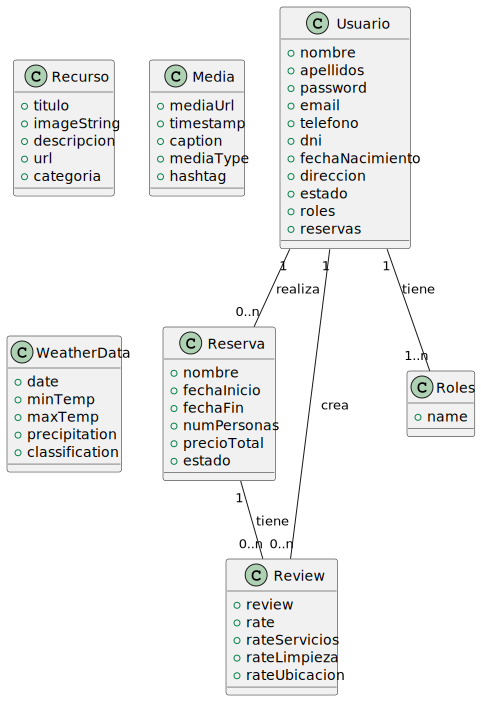
\includegraphics[width=1\textwidth]{figs/clases_simple.pdf}
    \caption{Diagrama general de clases.\label{fig:diagrama_clases}}
   
\end{figure}

\chapter{Diseño}
% Contenidos del capítulo.
% Las secciones presentadas son orientativas y no representan
% necesariamente la organización que debe tener este capítulo.

% Diagramas de clases, de secuencia, de despliegue, diseño de
% pantallas, etc

En esta sección se va a introducir el diseño o arquitectura del sistema mediante diagramas
de componentes de cada uno de los componentes lógicos que forman los subsistemas
de la aplicación. Además, se va a especificar diagramas de secuencia más precisos para
cada una de las funcionalidades de los componentes de cada subsistema. Para finalizar, se muestra un diagrama
de despliegue en el que se podrá observar los nodos a desplegar y el empaquetamiento de cada
componente.

\section{Arquitectura de componentes}

\subsection{Arquitectura de Componentes del Sistema Web}
La Figura~\ref{fig:componentes_sistema} muestra el diagrama de componentes del sistema desarrollado, el cual está estructurado en tres capas tecnológicas principales: \textbf{Frontend Web}, \textbf{Backend Principal} y \textbf{Subsistemas especializados y servicios externos}. Esta arquitectura modular permite una escalabilidad horizontal clara, así como la integración sencilla de nuevas funcionalidades.

\begin{sidewaysfigure}
    \centering
    \includegraphics[width=0.95\textheight]{figs/arquitectura.pdf}
    \caption{Diagrama de componentes del sistema.\label{fig:componentes_sistema}}
\end{sidewaysfigure}


\subsubsection*{1. Plataforma Web Frontend}
Implementada con \texttt{Angular} y tecnologías estándar como \texttt{HTML5}, la interfaz de usuario está compuesta por varios componentes funcionales:

\begin{itemize}
\item \textbf{Login}, \textbf{Register}, \textbf{Gestor}, \textbf{Inicio}, \textbf{Reservas}, \textbf{LaCasa}, \textbf{Entorno}, \textbf{Recomendaciones}, \textbf{ComoLlegar}:
Son los componentes visuales que representan cada una de las vistas principales.

\item \textbf{Servicios asociados}: cada vista se comunica con el backend a través de servicios como:
\begin{itemize}
    \item \texttt{AuthService}: gestión de autenticación y login.
    \item \texttt{RegistroService}: registro de usuarios.
    \item \texttt{ReserveService}: gestión de reservas.
    \item \texttt{WeatherService}: consulta de clima.
    \item \texttt{ContactoService}: envío de formularios de contacto.
    \item \texttt{ReviewService}: envío y recuperación de reseñas.
    \item \texttt{MediaService}: carga de publicaciones desde redes sociales.
    \item \texttt{EntornoService}: obtención de datos de recursos turísticos.
\end{itemize}
\end{itemize}

\subsubsection*{2. Sistema Principal Backend}
Este bloque implementa la lógica de negocio central mediante \texttt{Spring Boot}, \texttt{Spring WebFlux}, \texttt{Spring Security} y \texttt{Spring Data Reactive}. Sus componentes son:

\begin{itemize}
\item \textbf{Gestión de Reservas}: permite crear, actualizar y cancelar reservas, accediendo a la base de datos \texttt{PostgreSQL} mediante \texttt{R2DBC}.
\item \textbf{Seguridad y Autenticación}: implementada con \texttt{Spring Security} y \texttt{JWT}, garantiza la protección del acceso a recursos.
\item \textbf{Formulario de Contacto}: usa \texttt{JavaMailSender} para el envío de mensajes desde la web.
\item \textbf{Gestión de Reseñas}: permite a los usuarios enviar valoraciones sobre su experiencia.
\end{itemize}

Además, toda la persistencia en el sistema principal está delegada en la \textbf{base de datos SQL PostgreSQL}, que incluye las tablas \texttt{reservas}, \texttt{users/roles} y \texttt{reviews}.

\subsubsection*{3. Subsistemas especializados}
Los microservicios siguientes se encargan de tareas específicas, todos desarrollados con \texttt{Spring Boot} y tecnologías reactivas:

\begin{itemize}
\item \textbf{Subsistema de Publicaciones}:
\begin{itemize}
\item Conecta con la \textbf{API de Instagram Graph} para importar publicaciones según hashtags.
\item Almacena los datos en la colección \texttt{media} de \texttt{MongoDB}.
\end{itemize}

\item \textbf{Subsistema de Clima}:
\begin{itemize}
    \item Obtiene predicciones meteorológicas usando \textbf{Open Meteo API}.
    \item Los datos se almacenan en la colección \texttt{weatherData} en \texttt{MongoDB}.
\end{itemize}

\item \textbf{Subsistema de Recursos Municipales}:
\begin{itemize}
    \item Utiliza \texttt{JSoup} para extraer información desde \textbf{webs municipales y turísticas}.
    \item Almacena los resultados en la colección \texttt{recursos} en \texttt{MongoDB}.
\end{itemize}
\end{itemize}

\subsubsection*{4. Integraciones Externas}
\begin{itemize}
\item \textbf{Bases de datos NoSQL}: gestionadas con \texttt{MongoDB}, organizadas en colecciones específicas para medios, clima y entorno.
\item \textbf{APIs externas}: el sistema accede a fuentes de datos abiertas como \textbf{Instagram Graph API} y \textbf{Open Meteo API}.
\item \textbf{Recursos Web}: portales oficiales de entidades como \textit{Turisme Comunitat Valenciana} y \textit{Diputació de València}.
\end{itemize}


\section{Sistema principal}
En el sistema principal, el componente de reservas gestiona el flujo completo asociado a la realización y gestión de reservas por parte de los usuarios y del gestor. A continuación, se describen los diferentes procesos soportados, ilustrados mediante diagramas de secuencia.

\begin{itemize}

\item En la Figura~\ref{fig:secuencia_reserva_confirmacion}, se presenta el proceso de \textbf{confirmación de reserva}. Un \texttt{Usuario} envía una solicitud con los datos necesarios para registrar una reserva. El controlador valida los datos y consulta si el usuario existe en la base de datos. Tras almacenar la reserva en el repositorio, se envía un correo de confirmación mediante el servicio de correo electrónico. El sistema responde con un código \texttt{201 CREATED}.

\item La Figura~\ref{fig:secuencia_reserva_obtener} describe la \textbf{consulta de reservas por parte del gestor}. El \texttt{Gestor} solicita todas las reservas ordenadas por fecha de inicio. La lógica del servicio consulta el repositorio y retorna un \texttt{Flux\<Reserva\>} con los resultados.

\item En la Figura~\ref{fig:secuencia_reserva_proximas}, se representa el proceso de \textbf{obtención de reservas próximas}. En este caso, cualquier \texttt{Usuario} puede consultar las reservas a partir de la fecha actual. El sistema devuelve un \texttt{Flux\<Tuple2\<LocalDate, LocalDate\>} con los intervalos de fechas de las reservas, para que se visualicen los dias reservados en el calendario por otros usuarios.

\item La Figura~\ref{fig:secuencia_reserva_estado} detalla el flujo de \textbf{actualización del estado de una reserva}. El \texttt{Gestor} envía una petición para modificar el estado. Dependiendo del nuevo estado, se ejecutan acciones distintas: si se marca como \texttt{PAGADA}, se confirma el pago y se envía un correo de confirmación; si se marca como \texttt{CANCELADA}, se notifica la cancelación. En ambos casos, se actualiza la entidad y se guarda en la base de datos.

\item Por último, la Figura~\ref{fig:secuencia_reserva_usuario} ilustra la \textbf{consulta de reservas por usuario}. A través del correo electrónico, un \texttt{Usuario} puede recuperar sus reservas. El sistema filtra por email y responde con un \texttt{Flux\<Reserva\>}.

\end{itemize}


\begin{figure}[h!tb]
\centering
\includegraphics[width=\textwidth]{figs/secuencia_reserva_confirmacion.pdf}
\caption{Diagrama de secuencia - Confirmación de reserva.\label{fig:secuencia_reserva_confirmacion}}

\end{figure}

\begin{figure}[h!tb]
\centering
\includegraphics[width=\textwidth]{figs/secuencia_reserva_gestor_get.pdf}
\caption{Diagrama de secuencia - Obtener reservas (Gestor).\label{fig:secuencia_reserva_obtener}}
\end{figure}

\begin{figure}[h!tb]
\centering
\includegraphics[width=\textwidth]{figs/secuencia_reserva_proximas.pdf}
\caption{Diagrama de secuencia - Obtener reservas próximas.\label{fig:secuencia_reserva_proximas}}
\end{figure}

\begin{figure}[h!tb]
\centering
\includegraphics[width=\textwidth]{figs/secuencia_reserva_estado.pdf}
\caption{Diagrama de secuencia - Actualización de estado.\label{fig:secuencia_reserva_estado}}
\end{figure}

\begin{figure}[h!tb]
\centering
\includegraphics[width=\textwidth]{figs/secuencia_reserva_usuario.pdf}
\caption{Diagrama de secuencia - Obtener reservas por usuario.\label{fig:secuencia_reserva_usuario}}
\end{figure}
Después, se encuentra el componente de gestión de reseñas. En este módulo, los usuarios que hayan realizado una reserva (rol \texttt{CLIENTE}) podrán dejar reseñas en la aplicación, las cuales podrán ser consultadas por cualquier otro usuario. Este componente se divide en dos funcionalidades principales: añadir una reseña y consultar las reseñas existentes.

En la Figura~\ref{fig:secuencia_reseña_add} se representa el flujo completo para el proceso de añadir una reseña. El usuario autenticado, con rol CLIENTE, envía una solicitud \texttt{POST} con los datos de la reseña. El controlador delega la petición al servicio, que identifica al usuario por medio del sistema de autenticación de Spring y lo inyecta en la petición. Luego, se consulta el repositorio de usuarios para recuperar la entidad correspondiente y se elimina su rol de \texttt{CLIENTE}, dado que este rol es transitorio y únicamente se asigna tras una estancia validada. Posteriormente, se guarda la reseña en el repositorio de reseñas y se devuelve una respuesta de tipo \texttt{Mono\<ResponseEntity<Review\>\>} al cliente.

\begin{figure}[h!tb]
    \centering
    \includegraphics[width=\textwidth]{figs/secuencia_reseñas_bajo.pdf}
    \caption{Diagrama de secuencia del proceso de añadir una reseña.\label{fig:secuencia_reseña_add}}
\end{figure}

En la Figura~\ref{fig:secuencia_reseña_get} se ilustra el proceso de consulta de reseñas. En este caso, cualquier usuario puede enviar una solicitud \texttt{GET} para recuperar las reseñas almacenadas. El controlador redirige la petición al servicio, que a su vez consulta el repositorio de reseñas mediante una operación reactiva que devuelve un \texttt{Flux\<Review\>} ordenado por fecha de creación en orden descendente. La respuesta se entrega finalmente al cliente en forma de una lista de reseñas disponibles.

\begin{figure}[h!tb]
    \centering
    \includegraphics[width=\textwidth]{figs/secuencia_reseñas_get.pdf}
    \caption{Diagrama de secuencia del proceso de consulta de reseñas.\label{fig:secuencia_reseña_get}}
\end{figure}
A continuación, se encuentra el componente de contacto, el cual permite a los usuarios enviar mensajes directamente al administrador de la casa rural a través de un formulario. En la Figura~\ref{fig:secuencia_contacto} se observa el diseño de la lógica de este proceso. El usuario envía una solicitud \texttt{POST} con los datos del formulario, incluyendo nombre, email y mensaje. El controlador recibe la petición y delega el envío del correo al servicio correspondiente.

El \texttt{ContactService} construye un mensaje de tipo \texttt{SimpleMailMessage} utilizando los datos proporcionados por el usuario y lo envía mediante el componente \texttt{JavaMailSender}, el cual está configurado en el sistema. Una vez enviado el correo electrónico, el servicio devuelve una respuesta de tipo \texttt{Mono\<Contact>}, que es encapsulada en un objeto \texttt{ResponseEntity} para ser devuelta al usuario con un estado HTTP 200 si todo ha ido correctamente, o 400 en caso de error.

\begin{figure}[h!tb]
    \centering
    \includegraphics[width=\textwidth]{figs/secuencia_contacto.pdf}
    \caption{Diagrama de secuencia del componente de contacto.\label{fig:secuencia_contacto}}
\end{figure}

Finalmente, se encuentra el componente encargado de la seguridad el cual se especifica mediante configuración y infraestructura. Por lo tanto, se detallará en la sección de despliegue \ref{ch:despliegue} y en la implementación \ref{ch:im}
\section{Subsistema de recursos web}

En el subsistema de recursos web, uno de los componentes fundamentales es el servicio de raspado automatizado de contenidos turísticos. Este componente permite tanto a los usuarios acceder a los recursos almacenados como al sistema actualizar periódicamente la información mediante técnicas de \textit{web scraping}.

\subsection{Extracción solicitada por el usuario}

En la Figura~\ref{fig:secuencia_recursos_usuarios} se ilustra el comportamiento del sistema cuando un usuario interactúa con el \texttt{ExtraccionController} para consultar los recursos disponibles. Se representan dos casos diferenciados:

\begin{itemize}
  \item Una solicitud GET a \texttt{/api/v1/extraccion} desencadena la invocación del método \texttt{extractAllResources()} del servicio \texttt{RecursoService}, que accede a todos los documentos de la colección mediante el repositorio reactivo \texttt{RecursoRepository} y retorna un \texttt{Flux<Recurso>}.
  
  \item En el segundo caso, cuando el usuario realiza una solicitud GET a \texttt{/api/v1/extraccionFiestas}, el sistema filtra los resultados por la categoría \texttt{"fiestas"} mediante el método \texttt{findByCategoria()}.
\end{itemize}

\begin{figure}[h!tb]
    \centering
    \includegraphics[width=1\textwidth]{figs/secuencia_recursos_usuarios.pdf}
    \caption{Diagrama de secuencia para solicitudes de recursos por parte de usuarios.\label{fig:secuencia_recursos_usuarios}}
\end{figure}

\subsection{Extracción programada con scraping}

En la Figura~\ref{fig:secuencia_recursos_scheduled} se representa la lógica que ejecuta la tarea de extracción programada mediante un \texttt{@Scheduled} en el servicio \texttt{RecursoService}. Esta ejecución se realiza automáticamente cada día a las 00:00 horas y tiene como objetivo extraer y almacenar información actualizada desde diversas fuentes externas.

Durante este proceso:

\begin{itemize}
  \item Se invoca secuencialmente el método \texttt{scrape()} del \texttt{ScraperService}, pasando como parámetros la URL base, el tipo de recurso (como \texttt{"monumentos"}, \texttt{"fiestas"}) y la localización (como \texttt{chelva} o \texttt{tuejar}).
  \item Internamente se llama a \texttt{ensureCollectionExists()} para asegurar que la colección \texttt{recursos} existe en MongoDB usando \texttt{ReactiveMongoTemplate}.
  \item Se realiza una conexión con cada URL mediante \textbf{JSoup} y se procesan los resultados con métodos específicos como \texttt{processChelvaMonumentosAldeas()},\\ \texttt{processTuejarPatrimonioNaturaleza()}\\ o \texttt{processTuejarFiestas()}.
  \item Cada recurso se almacena en MongoDB a través del \texttt{RecursoRepository}.
  \item Finalmente, se consulta la base de datos para verificar el estado actualizado de todos los recursos.
\end{itemize}

\begin{figure}[h!tb]
    \centering
    \includegraphics[width=1\textwidth]{figs/secuencia_recursos_schedule.pdf}
    \caption{Diagrama de secuencia de la extracción programada de recursos web.\label{fig:secuencia_recursos_scheduled}}
\end{figure}

\section{Subsistema de publicaciones}

En el subsistema de publicaciones el componente a especificar es el encargado de realizar la llamada a la \gls{API} de Instagram para obtener publicaciones públicas. En la Figura~\ref{fig:secuencia_publicaciones_consulta} se representa cómo interactúan los distintos elementos del sistema para gestionar consultas, así como la extracción y actualización de publicaciones desde la red social.

Cuando un \textbf{usuario} realiza una solicitud GET a \texttt{/api/v1/media}, el \texttt{MediaController} llama al \texttt{MediaService}, que busca las publicaciones en el repositorio (\texttt{MediaRepository}). Si no se encuentra ninguna entrada relevante, el servicio puede invocar la \gls{API} de Instagram a través del cliente HTTP reactivo (\texttt{WebClient}), para recuperar y actualizar los datos de forma dinámica.

Además, este proceso de sincronización se ejecuta automáticamente cada día a las 00:00 mediante un temporizador (\texttt{Timer}). El servicio obtiene el token de acceso desde el sistema de archivos mediante el \texttt{InstagramTokenService}, realiza la solicitud a la \gls{API} de Instagram y, en función de si la publicación ya existe en la base de datos o no, realiza una de las siguientes acciones:

\begin{itemize}
    \item \textbf{Guardar nueva publicación:} Si el identificador no se encuentra registrado, se almacena la nueva publicación.
    \item \textbf{Actualizar publicación existente:} Si la publicación ya existe, se actualiza su URL de medios.
\end{itemize}

Este comportamiento condicional se resume mediante una estructura \texttt{alt} que permite distinguir entre ambos flujos. El resultado del proceso se devuelve al \texttt{Timer} como indicativo de finalización.

\begin{figure}[h!tb]
    \centering
    \includegraphics[width=1\textwidth]{figs/secuencia_publicaciones_baja.pdf}
    \caption{Diagrama de secuencia de consulta, extracción y actualización de publicaciones desde la \gls{API} de Instagram.\label{fig:secuencia_publicaciones_consulta}}
\end{figure}

Por otro lado, la Figura~\ref{fig:secuencia_publicaciones_token} muestra el procedimiento automatizado de renovación del token de acceso, esencial para mantener la conexión con la \gls{API}. Cada 30 días, el \texttt{InstagramTokenService} accede al sistema de archivos (\texttt{Filesystem}) para leer el token actual y realiza una solicitud a la ruta \texttt{refresh\_access\_token}. Una vez recibido el nuevo token, lo guarda de nuevo en el sistema de archivos. Este proceso garantiza la operatividad continua del sistema sin necesidad de intervención manual.

\begin{figure}[h!tb]
    \centering
    \includegraphics[width=1\textwidth]{figs/secuencia_publicaciones_token.pdf}
    \caption{Diagrama de secuencia del proceso de refresco del token de acceso (Subsistema de publicaciones).\label{fig:secuencia_publicaciones_token}}
\end{figure}


\section{Subsistema de previsión del tiempo}

En el subsistema de previsión del tiempo, el componente a especificar es el encargado de obtener información meteorológica de cara a la reserva del usuario. En la Figura~\ref{fig:secuencia_tiempo} se describe el proceso completo llevado a cabo cuando un usuario realiza una solicitud para consultar el pronóstico del tiempo en un rango de fechas determinado.

El flujo comienza cuando el \textbf{usuario} realiza una petición GET a \texttt{/api/v1/weather}, incluyendo dos parámetros de fecha. El \texttt{WeatherController} delega esta solicitud al \\ \texttt{WeatherService}, que realiza una iteración sobre cada fecha individual del rango indicado. Para cada una de estas fechas, primero intenta recuperar los datos desde la base de datos documental (\texttt{WeatherDataRepository}).

En caso de que los datos no se encuentren almacenados, el sistema evalúa si la fecha es histórica o si corresponde a una predicción futura. Si se trata de una fecha histórica (pasada o más allá de los próximos 15 días), se realiza una petición a la API de historial de Open Meteo. Si es una predicción (hasta 15 días en el futuro), se consulta la API de pronóstico. En ambos casos, la respuesta se procesa y se clasifica (por ejemplo: ``Lluvioso'', ``Frío'', ``Caluroso''...), y los datos resultantes se guardan en el repositorio para su reutilización futura.

Finalmente, el servicio devuelve todos los resultados al controlador, que responde al usuario con la lista de datos meteorológicos correspondiente.

\begin{figure}[h!tb]
    \centering
    \includegraphics[width=1\textwidth]{figs/secuencia_tiempo.png}
    \caption{Diagrama de secuencia del componente de obtención de previsión del tiempo (Subsistema de previsión del tiempo).\label{fig:secuencia_tiempo}}
\end{figure}


\section{Diagrama de clases}
\label{ch:clases}
La Figura~\ref{fig:clases_disenyo} presenta el diagrama de clases que describe las principales entidades de un sistema de gestión de usuarios, reservas, opiniones y recursos. Este diagrama es fundamental para la comprensión de cómo interactúan las diferentes clases en el sistema.

\begin{sidewaysfigure}
    \centering
    \includegraphics[width=0.8\textwidth]{figs/clases.pdf} 
    \caption{Diagrama de clases completo del sistema\label{fig:clases_disenyo}}
\end{sidewaysfigure}



Este diagrama muestra la estructura y relaciones entre las clases principales del sistema. La clase \texttt{Usuario} contiene atributos como nombre, apellidos, email, teléfono, entre otros. Esta clase también tiene métodos relacionados con el registro y obtención de usuarios y roles. La clase \texttt{Reserva} se encarga de la gestión de reservas, incluyendo la confirmación, cancelación y obtención de datos relacionados con las mismas. La clase \texttt{Review} gestiona las opiniones de los usuarios sobre los servicios, permitiendo registrar y obtener reseñas. Además, la clase \texttt{Recurso} gestiona los recursos de tipo información, como eventos y actividades, con métodos para obtener datos mediante scraping. La clase \texttt{Media} se encarga de manejar la información multimedia, como fotos y publicaciones en redes sociales, y la clase \texttt{WeatherData} almacena información relacionada con el clima, que puede ser consultada por rango de fechas.

Las relaciones entre las clases están representadas con las líneas de asociación. Por ejemplo, un \texttt{Usuario} puede tener múltiples \texttt{Reservas} y \texttt{Reviews}, mientras que una \texttt{Reserva} puede tener varias \texttt{Reviews}. Además, cada \texttt{Usuario} tiene uno o más \texttt{Roles}, los cuales determinan sus permisos dentro del sistema.

\section{Modelo de datos}

En cuanto a modelos de datos físicos se han definido tres modelos de datos para determinar las colecciones a generar en \texttt{MongoDB} y uno para las tablas relacionales en \texttt{PostgreSQL}. 

\subsection{Modelo físico de la base de datos relacional (\texttt{PostgreSQL})}

La Figura~\ref{fig:modelo_datos_postgres} muestra el modelo físico de datos de la base de datos relacional, implementado en \texttt{PostgreSQL}. El diagrama entidad-relación describe la estructura de las tablas, los campos principales y las relaciones de integridad referencial existentes en el sistema.

\begin{figure}[h!tb]
\centering
\includegraphics[width=0.6\textwidth]{figs/pg_sifico.pdf}
\caption{Modelo físico de la base de datos relacional \texttt{PostgreSQL}.\label{fig:modelo_datos_postgres}}
\end{figure}

El modelo se compone de las siguientes tablas:

\texttt{users}: Contiene los datos de los usuarios del sistema. Incluye campos como \texttt{id} (clave primaria, tipo \texttt{SERIAL}), \texttt{fecha\_nacimiento}, \texttt{estado}, \texttt{fecha\_registro}, \texttt{fecha\_modificacion}, \texttt{fecha\_baja}, \texttt{nombre}, \texttt{password}, \texttt{apellidos}, \texttt{email}, \texttt{telefono}, \texttt{dni} y \texttt{direccion}.\\
Nota: El campo \texttt{password} se almacena cifrado tanto a nivel de base de datos como a nivel de aplicación, siguiendo buenas prácticas de seguridad y protección de la información sensible de los usuarios. Esta tabla se encuentra referenciada por otras entidades.

\texttt{roles}: Define los posibles roles de usuario en el sistema. Está formada por el campo \texttt{id} (clave primaria, tipo \texttt{SERIAL}) y \texttt{name} (tipo \texttt{VARCHAR}, único).

\texttt{user\_role}: Tabla intermedia que implementa la relación muchos-a-muchos entre usuarios y roles. Incluye los campos \texttt{user\_id} y \texttt{role\_id}, ambos claves foráneas que referencian a las tablas \texttt{users} y \texttt{roles}, respectivamente.

\texttt{reviews}: Almacena las valoraciones de los usuarios. Incluye \texttt{id} (clave primaria), \texttt{review} (texto), \texttt{rate}, \texttt{rate\_servicios}, \texttt{rate\_limpieza}, \texttt{rate\_ubicacion} (todos de tipo \texttt{INTEGER}), \texttt{user\_id} (clave foránea a \texttt{users}) y \texttt{creation\_date} (timestamp).

\texttt{reservas}: Recoge la información de las reservas realizadas. Sus campos principales son \texttt{id} (clave primaria), \texttt{fecha\_inicio}, \texttt{fecha\_fin}, \texttt{num\_personas}, \texttt{usuario\_id} (clave foránea a \texttt{users}), \texttt{nombre}, \texttt{email}, \texttt{telefono}, \texttt{dni}, \texttt{precio\_total} y \texttt{estado}.

El diagrama incluye las relaciones de integridad referencial entre las tablas mediante claves foráneas (\texttt{user\_id}, \texttt{role\_id} y \texttt{usuario\_id}), asegurando la consistencia de los datos a través de las asociaciones indicadas.

\subsection{Modelo de datos de la base de datos no relacional \texttt{MongoDB}}

La Figura~\ref{fig:modelo_datos_mongodb} muestra el modelo físico de datos correspondiente a las colecciones de la base de datos \texttt{MongoDB} utilizadas en el sistema. El diagrama representa tres colecciones principales: \texttt{recursos}, \texttt{media} y \texttt{weather\_data}, cada una con su respectiva estructura de campos.

\begin{figure}[h!tb]
\centering
\includegraphics[width=0.6\textwidth]{figs/mongo_fisico.pdf}
\caption{Modelo físico de la base de datos no relacional \texttt{MongoDB}.\label{fig:modelo_datos_mongodb}}
\end{figure}


\texttt{recursos}: Esta colección contiene documentos identificados por el campo \texttt{\_id} (clave primaria), y almacena los siguientes atributos: \texttt{title}, \texttt{categoria}, \texttt{imageString}, \texttt{url}, \texttt{description} y \texttt{localizacion}, todos de tipo \texttt{String}.

\texttt{media}: Los documentos de la colección \texttt{media} disponen de los campos \texttt{\_id} (clave primaria), \texttt{mediaurl}, \texttt{timestamp}, \texttt{caption}, \texttt{mediatype} y \texttt{hashtag}, todos de tipo \texttt{String}. El campo \texttt{hashtag} está indexado, ya que en el desarrollo se van a realizar la mayoría de búsquedas a través de él, por lo que al indexarlo mejorará la velocidad en la búsqueda de documentos.

\texttt{weather\_data}: Cada documento en esta colección se identifica por el campo \texttt{date} (clave primaria, de tipo \texttt{String}), y contiene los campos \texttt{minTemp}, \texttt{maxTemp}, \texttt{precipitation} (de tipo \texttt{double}) y \texttt{classification} (de tipo \texttt{String}).

En el modelo presentado no existen relaciones explícitas entre colecciones, ya que MongoDB utiliza un enfoque orientado a documentos donde cada colección es independiente y puede escalar de manera autónoma. Los tipos de datos y claves principales están reflejados en el propio diagrama.

\section{Despliegue del sistema}\label{ch:despliegue}

El presente sistema está diseñado para ejecutarse sobre una arquitectura de contenedores orquestada con \gls{kubernetes}, de forma que pueda desplegarse en cualquier proveedor de servicios en la nube. 
En este apartado se detalla la infraestructura de despliegue propuesta, representada visualmente en la Figura~\ref{fig:diagrama_despliegue} mediante un diagrama de despliegue, que resume gráficamente la organización de los servicios, contenedores, volúmenes persistentes y conexiones internas en el clúster de Kubernetes.

\begin{sidewaysfigure}
    \centering
    \includegraphics[width=0.8\textwidth]{figs/despliegue-nube.pdf}
    \caption{Diagrama de despliegue del sistema basado en contenedores Docker sobre arquitectura Kubernetes.\label{fig:diagrama_despliegue}}
\end{sidewaysfigure}

El sistema se compone de una aplicación principal, encapsulada en un contenedor Docker bajo el nombre de \texttt{elrincondeeva}, desplegada como un \texttt{Deployment} en Kubernetes. Esta aplicación central es responsable de coordinar la lógica de negocio y canalizar las peticiones hacia los distintos \glspl{microservicio} del sistema: \texttt{Publicaciones}, \texttt{PrevisionDeTiempo} y \texttt{RecursosWeb}, también empaquetados como contenedores Docker y desplegados como pods independientes dentro del clúster.

La comunicación externa con el sistema se realiza a través de un \gls{ingress} que expone el servicio principal mediante protocolo \gls{https}. Este \texttt{Ingress Controller} actúa como único punto de entrada al sistema, redirigiendo las peticiones entrantes al contenedor correspondiente del servicio principal, aunque se mantiene la flexibilidad para exponer directamente otros servicios si fuera necesario en un futuro.

En cuanto al almacenamiento persistente, el sistema utiliza dos bases de datos. Por un lado, una instancia de \gls{postgresql} para la gestión de datos relacionales, asociada exclusivamente al contenedor principal. Esta base de datos se monta sobre un volumen persistente (\gls{pv}) y un reclamo (\gls{pvc}) propio, garantizando la durabilidad de los datos. Por otro lado, los microservicios de \texttt{Publicaciones}, \texttt{PrevisionDeTiempo} y \texttt{RecursosWeb} comparten una base de datos \gls{mongodb} desplegada como un único contenedor y montada igualmente sobre su propio par \texttt{PV}/\texttt{PVC}.

Una particularidad del microservicio \texttt{Publicaciones} es que requiere almacenar de forma persistente un \gls{token} de acceso para consultar la \gls{API} de Instagram. Para ello, se ha montado un volumen persistente específico (\texttt{token-pv}) a través de un \texttt{PVC}, que permite mantener dicho archivo de manera duradera. Esta solución evita el uso de \texttt{Secrets} o \texttt{ConfigMaps}, que no serían adecuados debido a la necesidad de escritura dinámica sobre el archivo.

\section{Despliegue en entorno local}

Durante la fase de desarrollo, se ha optado por un despliegue en entorno local que permite una ejecución sencilla de cada uno de los componentes del sistema sin depender de herramientas de orquestación como \gls{kubernetes} ni de contenedores \gls{docker}. En este modelo, cada microservicio se ejecuta como una aplicación independiente en la misma máquina o red local, y se comunican entre sí mediante llamadas HTTP directas a través de diferentes puertos.

La Figura~\ref{fig:diagrama_despliegue_local} muestra el diagrama de despliegue utilizado durante el desarrollo local. En este esquema, cada componente desarrollado con \gls{springboot} (\texttt{SistemaPrincipal}, \texttt{Publicaciones}, \texttt{PrevisionDeTiempo} y \texttt{RecursosWeb}) se ejecuta como una aplicación independiente, expuesta a través de su propio puerto. Asimismo, las bases de datos \gls{postgresql} y \gls{mongodb} se ejecutan como servicios locales tradicionales.

A diferencia de la arquitectura en la nube descrita anteriormente, donde las comunicaciones están encapsuladas y controladas mediante un \gls{ingress}, en el entorno local cada servicio es accesible desde el exterior a través de \texttt{localhost} y su respectivo puerto. Esto implica que cualquier consumidor que conozca el puerto puede acceder directamente a cualquiera de los servicios, lo cual reduce el aislamiento y la seguridad del sistema. En el modelo de nube, sin embargo, solo se permite el acceso desde Internet al servicio principal (\texttt{SistemaPrincipal}) gracias al uso del \gls{ingress} y protocolos seguros como \gls{https}.

Este enfoque local permite realizar pruebas y desarrollos de manera más rápida y sin necesidad de infraestructura adicional, aunque se recomienda restringir su uso a entornos controlados, dado que carece de mecanismos de seguridad avanzados.

\begin{figure}[h!tb]
    \centering
    \includegraphics[width=\textwidth]{figs/despliegue_local.png}
    \caption{Diagrama de despliegue del sistema en entorno local.\label{fig:diagrama_despliegue_local}}
\end{figure}


\chapter{Implementación y pruebas}

En este capítulo se describe la implementación de la aplicación. Se presenta la arquitectura del sistema, los subsistemas que componen el sistema principal y el subsistema de recursos web. Además, se describen los endpoints y servicios más relevantes, así como la persistencia y acceso a datos de cada uno de los subsistemas. También, se presentan detalles finales de cómo ha quedado la aplicación y su despliegue en el servidor. Finalmente, se presentan las pruebas realizadas para verificar el correcto funcionamiento de la aplicación y su despliegue en el servidor.
\section{Implementación sistema principal}\label{ch:im}
En esta sección se describen los subsistemas que componen el sistema principal de la aplicación. Se describen los subsistemas y sus interacciones y se muestran los fragmentos de código más importantes para el funcionamiento de la aplicación.
\subsection{Seguridad}
La aplicación cuenta con un sistema de autenticación y autorización de usuarios. Para ello se ha utilizado \texttt{Spring Security}~\cite{springsecurity}. Este subsistema permite gestionar los roles de los usuarios y las restricciones de acceso a los diferentes recursos de la aplicación. Se han definido los siguientes roles:
\begin{itemize}
    \item \texttt{ADMIN}: Requiere autenticación. Tiene acceso a todas las funcionalidades de la aplicación. Además, puede gestionar las reservas de los usuarios.
    \item \texttt{CLIENTE}: Requiere autenticación. Tiene acceso a las funcionalidades de hacer una nueva reserva y dejar reseñas en la aplicación. Accede a todo el contenido y a contenido propio dónde puede visualizar sus reservas actuales o pasadas. Además, podrá dejar una reseña cada vez que realice una reserva y esta se encuentre en estado finalizada.
    \item \texttt{USER}: Requiere autenticación. Tiene acceso a la funcionalidad de hacer una nueva reserva  en la aplicación. Accede a todo el contenido y a contenido propio dónde puede visualizar sus reservas actuales o pasadas.
    \item SIN USUARIO: este no es un rol definido dentro de las tablas del sistema. Dentro de el se encuentran solo las funcionalidades de solo lectura que no requieren autenticación y el sistema de registro o inicio de sesión.
\end{itemize}
El sistema permite la creación de usuarios, para esto se ha habilitado un endpoint de acceso libre desde el cual cualquier usuario anónimo, puede registrarse para obtener así el rol de USUARIO y un perfil en la aplicación. El Listado~\ref{lst:registroEndpoint} muestra el endpoint habilitado, en el cual se realiza una implementación reactiva del sistema de registro con gestión de errores que serán enviados al frontend para notificar al usuario. Además, también ha un servicio que se lanza inicialmente desde la clase de configuración \texttt{TestDataBaseConfiguration} que hace la misma función que el de usuarios pero para crear al usuario administrador. 
\begin{longlisting}
    \caption{Fichero de endpoints de creación de usuarios {\tt SignupController.java}}
    \inputminted[highlightlines={30}, firstline=20, lastline=45]{java}{../backend/elrincondeeva/elrincondeeva/src/main/java/es/uv/hemal/elrincondeeva/endpoints/SignupController.java}
    \label{lst:registroEndpoint}
\end{longlisting}
Este endpoint llamará a un servicio que se encargara de crear el usuario en la base de datos. El Listado~\ref{lst:servicioRegistro} muestra el servicio que se encarga de crear el usuario en la base de datos y enviar el correo al usuario. En la línea 32 se puede observar como se controla que no se pueda duplicar el usuario en el sistema, pese a que en base de datos también se encuentra incluida esta restricción. En la línea 37 se puede observar como se procede a cifrar la contraseña antes de almacenarla en la base de datos. Finalmente, en la línea 53 se observa el proceso de guardado del usuario con los datos provenientes del objeto \gls{dto} que han sido transformados a un objeto de tipo \texttt{\texttt{USER}} que es el que se almacena en la base de datos mediante el repositorio y el dominio generado.
\begin{longlisting}
    \caption{Fichero de servicio de creación de usuarios {\tt SignupService.java}}
    \inputminted[highlightlines={32,36,54}, firstline=29, lastline=64]{java}{../backend/elrincondeeva/elrincondeeva/src/main/java/es/uv/hemal/elrincondeeva/services/SignupService.java}
    \label{lst:servicioRegistro}
\end{longlisting}
El sistema de autenticación y autorización se basa en el uso de \gls{jwt} para la gestión de los tokens de acceso. El Listado~\ref{lst:jwt} muestra el fichero de configuración del sistema de seguridad, donde se observa como se han definido las rutas que no requieren autenticación y las rutas que requieren autenticación. En las lineas 75 a 82 se observa como están los diferentes endpoints con restricciones especiales en la aplicación. Los primeros que aparecen son los endpoints a los cuales todo usuario incluso los no registrados podrán acceder. En la línea 90 se observa el endpoint para añadir reseña que solo lo puede realizar un usuario autenticado que tenga el rol de \texttt{CLIENTE} y en la 91 se especifica que todos los demás endpoints a los que se llame deben hacerse con un usuario autenticado independientemente de su rol. Por otro lado, destacar que se ha incluido la política de \gls{cors} para permitir solo los métodos utilizados y una política especial en la línea 98 para exponer los tokens, roles y distintos campos que son necesarios para que desde el \gls{frontend} se puedan consultar en el momento que se necesite. Finalmente, se observa que se ha decidido realizar una reimplementación de las clases de Spring Security \cite{springsecurity} de forma reactiva para poder comprobar la autoría de los tokens con los usuarios almacenados en la base de datos. En el Apéndice \ref{ap:codigoseguridad}, en el Listado~\ref{lst:autenticacionfilter}, se puede observar la implementación personalizada que se ha realizado validando el token \gls{jwt} con un objeto \texttt{USER} el cual internamente valida mediante un repositorio si existe en la base de datos. Finalmente, en el Apéndice \ref{ap:codigoseguridad}, en el Listado~\ref{lst:autorizacionfilter}, se realiza el filtro de autorización en caso de no ser un inicio de sesión y se extraen los roles que van implícitos en las propias peticiones y se obtiene el usuario directamente del \gls{jwt} para así identificar unívocamente cada petición con el usuario y acceder solamente a la información de este. 
\begin{longlisting}
    \caption{Fichero de configuración de seguridad {\tt WebSecurityConfig.java}}
    \inputminted[highlightlines={75-82,98}, firstline=36, lastline=111]{java}{../backend/elrincondeeva/elrincondeeva/src/main/java/es/uv/hemal/elrincondeeva/config/WebSecurityConfig.java}
    \label{lst:jwt}
\end{longlisting}

\subsection{Gestión de reservas}
En este apartado se describe el subsistema de gestión de reservas. Este subsistema permite gestionar las reservas de los usuarios y la disponibilidad de la casa rural. El desarrollo de este subsistema se divide en endpoints dedicados a los usuarios con rol \texttt{USER} y, por otro lado, endpoints dedicados a los usuarios con rol \texttt{ADMIN}, que permiten gestionar las peticiones de reserva generadas por los usuarios registrados.

Los usuarios autenticados con el rol \texttt{USER} podrán realizar nuevas reservas a través del endpoint \texttt{/reserva}, línea 33 del Listado~\ref{lst:reservaController}, que recoge los datos de una reserva y los procesa de forma reactiva mediante el servicio correspondiente. También podrán consultar las reservas que han realizado previamente mediante el endpoint \texttt{/reservasUser}, utilizando su dirección de correo electrónico como identificador (línea 83 del mismo listado), la cuál ha sido extradida por el \gls{frontend} con la llamada a un endpoint de información del usuario (/me) en función del token de autenticación.

En cuanto a los usuarios con el rol \texttt{ADMIN}, estos disponen de varios endpoints protegidos mediante la anotación \texttt{@PreAuthorize(``hasRole(ADMIN)``)}, lo cual restringe su uso exclusivamente a administradores. Uno de ellos es \texttt{/reservas}, que permite consultar todas las reservas realizadas por los usuarios (línea 50), y otro es \texttt{/reservasProximas}, que proporciona un listado de las reservas activas próximas a la fecha actual (línea 55). Además, el endpoint \texttt{/\{id\}/estado} (línea 71) permite modificar el estado de una reserva concreta, proporcionando tanto el nuevo estado como el motivo de la modificación.

El Listado~\ref{lst:reservaController} muestra el fichero completo \texttt{ReservaController.java}, el cual agrupa todos los endpoints descritos. En él se observa cómo se hace uso de la programación reactiva, y cómo se gestionan los errores de manera asíncrona, devolviendo respuestas adecuadas con los códigos de estado correspondientes.

\begin{longlisting}
    \caption{Fichero controlador de reservas {\tt ReservaController.java}}
    \inputminted[highlightlines={33,71,50,61,83}, firstline=26]{java}{../backend/elrincondeeva/elrincondeeva/src/main/java/es/uv/hemal/elrincondeeva/endpoints/ReservaController.java}
    \label{lst:reservaController}
\end{longlisting}


El Listado~\ref{lst:reservaService} muestra el fichero completo \texttt{ReservaService.java}, el cual implementa la lógica de negocio relacionada con la gestión de reservas. Este servicio es invocado por el controlador \texttt{ReservaController} (véase el Listado~\ref{lst:reservaController}) para realizar las operaciones sobre las reservas, incluyendo su creación, modificación, cancelación, confirmación de pago y actualización de roles de usuario.


\begin{longlisting} 
    \caption{Fichero de servicio de reservas {\tt ReservaService.java}} 
    \inputminted[firstline=25]{java}{../backend/elrincondeeva/elrincondeeva/src/main/java/es/uv/hemal/elrincondeeva/services/ReservaService.java} 
    \label{lst:reservaService} 
\end{longlisting}

A lo largo de la implementación se observa cómo se emplea programación reactiva gracias a los tipos \texttt{Mono<T>} y \texttt{Flux<T>}, lo que permite manejar flujos de datos de forma asíncrona y no bloqueante.

\begin{itemize}
    \item El método \texttt{confirmarReserva} crea una nueva reserva a partir de los datos proporcionados en un \texttt{ReservaDTO}, la asocia al usuario correspondiente a partir de su email, la guarda en la base de datos y finalmente lanza un correo de confirmación utilizando \texttt{EmailService} que se muestra en el Apéndice \ref{ap:emailservice}, Listado~\ref{lst:emailService}.
    
    \item El método \texttt{confirmarPagoReserva} se utiliza para marcar una reserva como pagada y enviar un correo de confirmación del pago. 
    
    \item De manera similar, \texttt{cancelarReserva} notifica por correo electrónico que una reserva ha sido cancelada.

    \item El método \texttt{setEstado} permite cambiar el estado de una reserva a través de su identificador, y según el nuevo estado, desencadena acciones adicionales como el envío de correos o la modificación de datos en la base.

    \item \texttt{getReservas} devuelve un flujo de identificadores de todas las reservas almacenadas, mientras que \texttt{getAllDataReservas} proporciona todos los datos completos de cada una de ellas.

    \item \texttt{getAllDataReservasFromToday} filtra aquellas reservas cuya fecha de inicio es igual o posterior al día actual, devolviendo únicamente sus intervalos de fechas, lo que puede ser útil para mostrar disponibilidad en un calendario.

    \item \texttt{getReservasByUser} permite obtener las reservas asociadas a un usuario concreto mediante su correo electrónico.

    \item Finalmente, el método programado \texttt{actualizarRolesUsuarios}, que se ejecuta automáticamente cada día a las 2:00h gracias a la anotación \texttt{@Scheduled}, actualiza el rol de los usuarios que hayan realizado reservas ya finalizadas, asignándoles el rol de cliente (\texttt{CLIENTE}) si todavía no lo tienen. Esta lógica garantiza que los usuarios activos que han completado reservas reciban un rol adecuado para su perfil y puedan dejar una reseña.
\end{itemize}


\subsection{Gestión de reseñas}
El subsistema de reseñas permite a los usuarios compartir valoraciones sobre su experiencia en la casa rural. Está compuesto por dos endpoints principales: uno para la consulta pública de reseñas y otro restringido para la creación de nuevas valoraciones.

El primer endpoint, \texttt{/reviews} línea 76 del Listado~\ref{lst:reviewController}, permite obtener todas las reseñas almacenadas en la base de datos, ordenadas de forma descendente según la fecha de creación. Este endpoint está disponible para cualquier usuario, sin necesidad de autenticación previa, lo que facilita la visibilidad de las opiniones existentes sobre el alojamiento.

El segundo endpoint, \texttt{/addReview} (línea 80), permite a los usuarios autenticados con el rol \texttt{CLIENTE} enviar una nueva reseña mediante un objeto \texttt{ReviewDTO}. Para ello, se obtiene el contexto de seguridad reactivo a fin de identificar al usuario autenticado, y se valida su existencia en la base de datos. A continuación, se construye un nuevo objeto \texttt{Review} con los datos proporcionados, incluyendo la puntuación general y las valoraciones específicas sobre limpieza, ubicación y servicios. Como paso final, se elimina la relación del usuario con el rol \texttt{ROLE\_CLIENTE} (línea 51), indicando que ya ha realizado su valoración, y se guarda la reseña en la base de datos. En caso de producirse un error durante este proceso, se responde con un código de estado \texttt{Bad Request}.

El Listado~\ref{lst:reviewController} muestra parte del fichero \texttt{ApplicationController.java} que contiene los endpoints para la gestión de reseñas, mientras que el Listado~\ref{lst:reviewService} recoge el contenido del servicio \texttt{ReviewService}, encargado de la lógica de negocio para almacenar y recuperar reseñas.

\begin{longlisting} 
    \caption{Endpoints para la gestión de reseñas {\tt ApplicationController.java}} 
    \inputminted[firstline=75,lastline=85]{java}{../backend/elrincondeeva/elrincondeeva/src/main/java/es/uv/hemal/elrincondeeva/endpoints/ApplicationController.java} 
    \label{lst:reviewController} 
\end{longlisting}

\begin{longlisting}
    \caption{Servicio de gestión de reseñas {\tt ReviewService.java}}
    \inputminted[firstline=18]{java}{../backend/elrincondeeva/elrincondeeva/src/main/java/es/uv/hemal/elrincondeeva/services/ReviewService.java}
    \label{lst:reviewService}
\end{longlisting}


\subsection{Formulario de contacto}
La aplicación incorpora un mecanismo de contacto que permite a cualquier usuario enviar un mensaje al propietario de la casa rural. Este mecanismo está disponible a través del endpoint \texttt{/contact}, que acepta solicitudes POST con un objeto \texttt{Contact} en formato \gls{json}.

El controlador delega la lógica de envío al servicio \texttt{ContactService}, el cual se encarga de construir y enviar un mensaje de correo electrónico a la dirección configurada en el sistema (a través de la propiedad \texttt{spring.email.email}). El contenido del mensaje incluye el nombre del remitente, su dirección de correo electrónico (usada como \texttt{reply-to}) y el mensaje de consulta proporcionado por el usuario.

Este servicio permite una comunicación directa entre los usuarios y el responsable del alojamiento, facilitando la resolución de dudas o la solicitud de información adicional sin necesidad de registro o autenticación previa.

A continuación, se muestran en el Listado~\ref{lst:contactController} las líneas relevantes del controlador \texttt{ApplicationController.java}, y en el Listado~\ref{lst:contactService} el fragmento correspondiente del servicio \texttt{ContactService.java}.

\begin{longlisting}
    \caption{Controlador de contacto {\tt ApplicationController.java}}
    \inputminted[ firstline=93, lastline=100]{java}{../backend/elrincondeeva/elrincondeeva/src/main/java/es/uv/hemal/elrincondeeva/endpoints/ApplicationController.java}
    \label{lst:contactController}
\end{longlisting}

\begin{longlisting}
    \caption{Servicio de contacto {\tt ContactService.java}}
    \inputminted[ firstline=15, lastline=55]{java}{../backend/elrincondeeva/elrincondeeva/src/main/java/es/uv/hemal/elrincondeeva/services/ContactService.java}
    \label{lst:contactService}
\end{longlisting}

\subsection{Persistencia y acceso a datos sistema principal}
Por último, se presenta la base de datos del sistema principal. Esta base de datos está compuesta por varias tablas que almacenan la información necesaria para el funcionamiento de la aplicación. A continuación, se describen las tablas más relevantes y los repositorios de Spring Data que permiten interactuar con ellas.
Para dar soporte a las operaciones del sistema, se han definido diversas entidades persistentes que se almacenan en una base de datos relacional PostgreSQL. Las tablas se crean a través del script \texttt{schema.sql}, el cual se ejecuta al iniciar la aplicación si las tablas no existen. A continuación se describe la estructura de cada una de las tablas principales y su relación con las clases del dominio y los repositorios correspondientes.


\begin{itemize}
    \item Entidad \texttt{Reserva}: La entidad \texttt{Reserva} representa una solicitud de reserva por parte de un usuario, e incluye información sobre las fechas, el número de personas, el estado de la reserva y los datos de contacto. Su representación en base de datos se define mediante la tabla \texttt{reservas}, incluida en el Listado~\ref{lst:reservasTable}. Esta tabla establece una relación de clave foránea con la tabla \texttt{users}, de forma que cada reserva está asociada a un usuario registrado.
  \begin{longlisting}
        \caption{Definición de la tabla \texttt{reservas} en {\tt schema.sql}}
        \inputminted[firstline=42,lastline=55]{sql}{../backend/elrincondeeva/elrincondeeva/src/main/resources/schema.sql}
        \label{lst:reservasTable}
    \end{longlisting}
    El acceso a esta entidad se realiza mediante el repositorio \texttt{ReservaRepository}, que extiende la interfaz \texttt{R2dbcRepository} y proporciona métodos para consultar reservas por identificador, estado, fecha de inicio o dirección de correo electrónico (véase Apéndice \ref{ap:persistenciaprincipal}, Listado~\ref{lst:reservaRepository}). La clase del dominio asociada es \texttt{Reserva}, que contiene los campos mapeados mediante anotaciones de Spring Data R2DBC (véase Apéndice \ref{ap:persistenciaprincipal}, Listado~\ref{lst:reservaDomain}).
    
    
    \item Entidad \texttt{Review}: La tabla \texttt{reviews}, Listado~\ref{lst:reviewsTable}, permite almacenar valoraciones realizadas por los usuarios sobre su experiencia en la casa rural. Cada reseña incluye un comentario textual, puntuaciones detalladas (servicios, limpieza y ubicación) y una relación directa con el usuario que la creó. Esta tabla también define una clave foránea a la tabla \texttt{users}, lo que asegura la integridad referencial.
     \begin{longlisting}
        \caption{Definición de la tabla \texttt{reviews} en {\tt schema.sql}}
        \inputminted[firstline=30,lastline=40]{sql}{../backend/elrincondeeva/elrincondeeva/src/main/resources/schema.sql}
        \label{lst:reviewsTable}
    \end{longlisting}
    El repositorio correspondiente, así como su dominio \texttt{Review}, se incluyen en el Apéndice~\ref{ap:persistenciaprincipal}, Listado~\ref{lst:reviewDomain} y Listado~\ref{lst:reviewRepository} para consulta detallada.
    
   
    \item Entidad \texttt{User} y control de roles: 

   En el Listado~\ref{lst:usersTable} se observan las siguientes tablas:

\begin{itemize}
    \item La tabla \texttt{users}, que representa a los usuarios del sistema, contiene información personal, de contacto y de estado de actividad.
    
    \item La relación de roles se gestiona mediante las tablas \texttt{roles} y \texttt{user\_role}, que permiten definir una estructura de autorización flexible mediante una relación de muchos a muchos. Además, dado que Spring R2DBC no admite campos que almacenen tipos de datos complejos, esta es la única forma viable de implementar dicha relación entre roles y usuarios.
\end{itemize}
 \begin{longlisting}
        \caption{Definición de las tablas \texttt{users}, \texttt{roles} y \texttt{user\_role} en {\tt schema.sql}}
        \inputminted[firstline=1,lastline=28]{sql}{../backend/elrincondeeva/elrincondeeva/src/main/resources/schema.sql}
        \label{lst:usersTable}
    \end{longlisting}
    Esta estructura es fundamental para la gestión de accesos a diferentes funcionalidades del sistema, como se ha visto en las secciones anteriores. Los repositorios correspondientes a estas entidades (\texttt{UserRepository}, \texttt{RoleRepository}, etc.) también se incluyen en el Apéndice~\ref{ap:persistenciaprincipal}.
    
    
\end{itemize}



\section{Subsistema de recursos web}
La aplicación incluye un mecanismo automatizado de extracción de recursos turísticos que permite mantener actualizada la información sobre sitios de interés cercanos a la casa rural. Este sistema está accesible mediante el controlador \texttt{ExtraccionController} del Listado~\ref{lst:extraccionController}, disponible en el endpoint \texttt{/extraccion}, y se apoya en el servicio \texttt{RecursoService} para obtener y devolver los datos en formato reactivo.

El controlador ofrece tres rutas distintas:

\texttt{/extraccion} para obtener todos los recursos turísticos conocidos,

\texttt{/extraccionFiestas} para obtener únicamente fiestas locales extraídas de sitios web oficiales,

\texttt{/extraccion/test} para forzar manualmente el scraping y almacenamiento de datos, útil para pruebas o actualizaciones no programadas.

La lógica principal reside en el servicio \texttt{RecursoService}, Listado~\ref{lst:recursoService}, el cual ejecuta una tarea programada diariamente mediante una anotación \texttt{@Scheduled}. Este servicio llama al \texttt{ScraperService}, que se encarga de realizar la extracción asíncrona de información desde diversas URLs predefinidas, seleccionadas tras un estudio previo de fuentes confiables, utilizando expresiones regulares de búsqueda \gls{css} o \gls{xpath} y la librería JSoup~\cite{jsoup}. La información extraída se procesa y guarda automáticamente en colecciones MongoDB\cite{mongodb} utilizando un repositorio reactivo.

Posteriormente, el propio \texttt{RecursoService}, presenta la lógica del servicio de recursos que consulta estas colecciones para proporcionar datos actualizados al usuario final, distinguiendo entre fiestas locales y otros eventos o lugares de interés, y en el Apéndice~\ref{ap:extraccion}, Listado~\ref{lst:scraperService} el servicio encargado de la extracción de estos datos de las fuentes correspondientes.

\begin{longlisting} \caption{Fragmento del controlador de extracción de recursos {\tt ExtraccionController.java}} \inputminted[firstline=15]{java}{../backend/extraccion/extraccion/src/main/java/es/uv/hemal/extraccion/extraccion/endpoints/ExtraccionController.java} \label{lst:extraccionController} \end{longlisting}

\begin{longlisting} \caption{Servicio para la gestión de recursos {\tt RecursoService.java}} \inputminted[firstline=13]{java}{../backend/extraccion/extraccion/src/main/java/es/uv/hemal/extraccion/extraccion/services/RecursoService.java} \label{lst:recursoService} \end{longlisting}

\subsection{Persistencia y acceso a datos subsistema de recursos web}
La persistencia de los recursos extraídos se realiza automáticamente mediante la integración con MongoDB a través de Spring Data Reactive. La entidad principal utilizada es \texttt{Recurso} (véase el Listado~\ref{lst:modelRecurso}), representada como un documento en la colección \texttt{recursos}, definida mediante la anotación \texttt{@Document} en la clase correspondiente.

Cada recurso incluye atributos como título, descripción, URL, imagen codificada en base64, localización y categoría. Para garantizar la unicidad de los registros, el identificador del documento se genera concatenando el título y la localización, lo que evita duplicados si se extrae un mismo sitio desde diferentes fuentes.

Además, la clase auxiliar \texttt{ScraperResult} (véase el Listado~\ref{lst:modelScraperResult}) encapsula una lista de objetos \texttt{Recurso} obtenidos tras realizar el proceso de extracción desde fuentes externas. Esta estructura intermedia permite manejar de forma más flexible los resultados antes de su inserción en la base de datos.

El acceso a la base de datos se gestiona mediante el repositorio reactivo \texttt{RecursoRepository}, que extiende la interfaz \texttt{ReactiveMongoRepository}. Este repositorio expone métodos personalizados como \texttt{findByTitle} y \texttt{findByCategoria}, que permiten realizar búsquedas específicas dentro de la colección \texttt{recursos} sin necesidad de definir consultas manualmente (Listado~\ref{lst:recursoRepository}).

Gracias al uso de estas herramientas, las colecciones se crean automáticamente al insertar el primer documento, eliminando la necesidad de una definición previa o scripts de inicialización.

\begin{longlisting} \caption{Modelo de documento MongoDB para recursos turísticos {\tt Recurso.java}} \inputminted[firstline=6,lastline=78]{java}{../backend/extraccion/extraccion/src/main/java/es/uv/hemal/extraccion/extraccion/models/Recurso.java} \label{lst:modelRecurso} \end{longlisting}

\begin{longlisting} \caption{Modelo auxiliar de resultados de scraping {\tt ScraperResult.java}} \inputminted[firstline=6,lastline=33]{java}{../backend/extraccion/extraccion/src/main/java/es/uv/hemal/extraccion/extraccion/models/ScraperResult.java} \label{lst:modelScraperResult} \end{longlisting}

\begin{longlisting} 
  \caption{Repositorio para la persistencia en MongoDB {\tt RecursoRepository.java}} 
  \inputminted[firstline=5,lastline=13]{java}{../backend/extraccion/extraccion/src/main/java/es/uv/hemal/extraccion/extraccion/repositories/RecursoRepository.java} \label{lst:recursoRepository} \end{longlisting}
\section{Subsistema de publicaciones}
Este subsistema está diseñado para obtener publicaciones desde la API de Instagram, procesarlas y almacenarlas en una base de datos MongoDB. Para ello se utilizan controladores y servicios desarrollados en Spring Boot utilizando Spring WebFlux~\cite{webflux} de forma reactiva.

\subsubsection{Controlador de publicaciones}

El controlador principal expone los endpoints para la consulta y extracción de publicaciones, así como la actualización de información asociada. El código se muestra en el listado~\ref{lst:mediaController}.

\begin{longlisting}
\caption{Controlador principal para las publicaciones {\tt MediaController.java}}
\inputminted[
    firstline=14
]{java}{../backend/PublicacionesAPI/PublicacionesAPI/src/main/java/es/uv/hemal/elrincondeeva/PublicacionesAPI/controllers/MediaController.java}
\label{lst:mediaController}
\end{longlisting}

Entre sus funcionalidades destacadas se encuentran:

\begin{itemize}
    \item \texttt{/media}: devuelve todas las publicaciones almacenadas.
    \item \texttt{/media/hashtag/\{hashtag\}}: permite filtrar publicaciones por hashtag.
    \item \texttt{/media/test}: ejecuta manualmente la extracción desde Instagram.
\end{itemize}

\subsubsection{Servicio de extracción de publicaciones}

El servicio contiene la lógica de negocio encargada de conectarse con la API de Instagram, extraer las publicaciones, procesar su contenido y guardarlo en la base de datos. Su implementación se detalla en el Listado~\ref{lst:mediaService}.

\begin{longlisting}
\caption{Servicio de extracción y almacenamiento de publicaciones {\tt MediaService.java}}
\inputminted[
    firstline=23
]{java}{../backend/PublicacionesAPI/PublicacionesAPI/src/main/java/es/uv/hemal/elrincondeeva/PublicacionesAPI/services/MediaService.java}
\label{lst:mediaService}
\end{longlisting}

En este servicio se pueden destacar los siguientes métodos clave:

\begin{itemize}
    \item \textbf{\texttt{fetchAndStorePosts()}}: realiza la conexión con Instagram y obtiene las publicaciones.
    \item \textbf{\texttt{processAndStorePost(post)}}: comprueba si ya existe en la base de datos, y en caso contrario, la almacena o si existe actualiza el timestamp y la url, ya que al guardarse las imágenes en una \gls{cdn}, Instagram las elimina cada cierto tiempo y hay que renovar la URL.
    \item \textbf{\texttt{extractHashtags(caption)}}: extrae todos los hashtags de una publicación mediante expresiones regulares.
    \item \textbf{\texttt{savePostWithHashtags(post, hashtags)}}: almacena la publicación junto con los hashtags en MongoDB.
\end{itemize}

Cuando se invoca el método \texttt{fetchAndStorePosts()}, el servicio realiza una petición a la API de Instagram Graph \cite{api:instagram} obteniendo los datos en formato \gls{json}. A continuación, por cada publicación:

\begin{enumerate}
    \item Se extraen los campos relevantes: ID, texto, medios, y hashtags.
    \item Se verifica si esa publicación ya existe en la base de datos.
    \item Si es nueva, se guarda junto con los hashtags en un documento MongoDB.
\end{enumerate}

Por último, existe una clase encargada de refrescar el token de acceso a la API de Instagram, que se invoca cada 50 dias para garantizar el acceso continuo a los datos. Estos tokens serán gestionados en un fichero cuya ruta estará definida en las propiedades de cada entorno (Véase en Apéndice~\ref{ap:instagramtoken}, Listado~\ref{lst:refreshToken}).


\subsubsection{Persistencia y acceso a datos subsistema de publicaciones}
La persistencia de los medios extraídos de Instagram se realiza automáticamente mediante la integración con MongoDB a través de Spring Data Reactive. La entidad principal utilizada es \texttt{Media} (véase el Listado~\ref{lst:modelMedia}), representada como un documento en la colección \texttt{media}, definida mediante la anotación \texttt{@Document} en la clase correspondiente.

Cada medio incluye atributos como \texttt{mediaurl} (URL del medio), \texttt{timestamp} (fecha y hora de publicación), \texttt{caption} (descripción del medio), \texttt{mediatype} (tipo de medio) y \texttt{hashtag} (etiqueta asociada). Para garantizar la unicidad de los registros, el identificador del documento es el id generado por el sistema origen (Instagram).

La clase auxiliar \texttt{MediaRepository} del Listado~\ref{lst:mediaRepository}, extiende \texttt{ReactiveMongoRepository}, lo que permite realizar operaciones reactivas sobre la base de datos sin necesidad de escribir consultas SQL tradicionales. Este repositorio expone métodos personalizados como \texttt{findByHashtag}, que permiten realizar búsquedas específicas dentro de la colección \texttt{media}.

El acceso a la base de datos es completamente reactivo, lo que optimiza la interacción con MongoDB y permite manejar grandes volúmenes de datos de manera eficiente.

\begin{longlisting} 
\caption{Modelo de documento MongoDB para los medios {\tt Media.java}} 
\inputminted[firstline=6,lastline=30]{java}{../backend/PublicacionesAPI/PublicacionesAPI/src/main/java/es/uv/hemal/elrincondeeva/PublicacionesAPI/domain/Media.java} 
\label{lst:modelMedia} 
\end{longlisting}

\begin{longlisting} 
\caption{Repositorio para la persistencia en MongoDB {\tt MediaRepository.java}} 
\inputminted[firstline=5,lastline=9]{java}{../backend/PublicacionesAPI/PublicacionesAPI/src/main/java/es/uv/hemal/elrincondeeva/PublicacionesAPI/repositories/MediaRepository.java} 
\label{lst:mediaRepository} 
\end{longlisting}

\section{Subsistema de extracción de datos meteorológicos} 
El sistema de extracción de datos meteorológicos obtiene información sobre el clima de una región específica en base a un rango de fechas proporcionado por el usuario. Este subsistema está accesible mediante el controlador \texttt{WeatherController} disponible en el endpoint \texttt{/weather}, y se apoya en el servicio \texttt{WeatherService} para obtener y devolver los datos en formato reactivo.

El controlador ofrece una ruta principal:

\texttt{/weather} para obtener datos meteorológicos de un rango de fechas proporcionado por el usuario, usando parámetros \texttt{startDate} y \texttt{endDate} en formato de fecha \gls{iso}.

La lógica principal reside en el servicio \texttt{WeatherService}, el cual se encarga de obtener los datos meteorológicos desde la API de Open-Meteo~\cite{openmeteo:2025}. Si los datos no están disponibles en la base de datos, el servicio consulta la API para obtener la información histórica o pronosticada, dependiendo de la fecha proporcionada. Los datos obtenidos incluyen la temperatura máxima, mínima y la precipitación, y se clasifican como ``Lluvioso``, ``Caluroso``, ``Frío`` o ``Normal``, según las condiciones climáticas.

A continuación, se presentan los fragmentos relevantes de implementación. En el Listado~\ref{lst:weatherController} se presenta el controlador de datos meteorológicos, en el Listado~\ref{lst:weatherService} la lógica del servicio de extracción de datos meteorológicos, y en el Listado~\ref{lst:weatherRepository} el repositorio encargado de la persistencia en MongoDB~\cite{mongodb}.

\begin{longlisting} \caption{Fragmento del controlador de datos meteorológicos {\tt WeatherController.java}} \inputminted[firstline=15]{java}{../backend/tiempo/tiempo/src/main/java/hemal/uv/es/tiempo/controllers/WeatherController.java} \label{lst:weatherController} \end{longlisting}

\begin{longlisting} \caption{Servicio para la gestión de datos meteorológicos {\tt WeatherService.java}} \inputminted[firstline=18,fontsize=\small, breaklines, breakanywhere]{java}{../backend/tiempo/tiempo/src/main/java/hemal/uv/es/tiempo/services/WeatherService.java} \label{lst:weatherService} \end{longlisting}

\subsubsection{Persistencia y acceso a datos en el subsistema de extracción de datos meteorológicos} 

La persistencia de los datos meteorológicos se realiza automáticamente mediante la integración con MongoDB a través de Spring Data Reactive. La entidad principal utilizada es \texttt{WeatherData}, representada como un documento en la colección \texttt{weather\_data}, definida mediante la anotación \texttt{@Document} en la clase correspondiente.

Cada entrada de datos meteorológicos incluye atributos como fecha, temperatura mínima, temperatura máxima, precipitación y clasificación del día. El identificador del documento se corresponde con la fecha, lo que garantiza que no haya duplicados para una misma fecha.

El acceso a la base de datos se gestiona mediante el repositorio reactivo \texttt{WeatherDataRepository}, que extiende la interfaz \texttt{ReactiveMongoRepository}. Este repositorio permite realizar búsquedas específicas dentro de la colección \texttt{weather\_data} mediante consultas como \texttt{findByDate}, sin necesidad de definir consultas manualmente.

Gracias a esta integración, los datos meteorológicos se guardan y recuperan de forma eficiente, permitiendo consultas rápidas y actualizadas.

A continuación, en el Listado~\ref{lst:modelWeatherData} se presentan los fragmentos relevantes de las clases de modelo y en el Listado~\ref{lst:weatherRepository} los más relevantes del repositorio.

\begin{longlisting} \caption{Modelo de documento MongoDB para datos meteorológicos {\tt WeatherData.java}} \inputminted[firstline=6]{java}{../backend/tiempo/tiempo/src/main/java/hemal/uv/es/tiempo/domain/WeatherData.java} \label{lst:modelWeatherData} \end{longlisting}

\begin{longlisting} \caption{Repositorio de datos meteorológicos {\tt WeatherDataRepository.java}} \inputminted{java}{../backend/tiempo/tiempo/src/main/java/hemal/uv/es/tiempo/repositories/WeatherDataRepository.java} \label{lst:weatherRepository} \end{longlisting}

\section{Aplicación \gls{frontend} y diseño de la interfaz de usuario}
En esta sección se describen los principales componentes que conforman la implementación del \gls{frontend} de la aplicación, incluyendo tanto los componentes como los servicios desarrollados. Asimismo, se presenta el diseño final de dichos elementos, mostrando el resultado visual y funcional alcanzado tras su integración.
\subsection{Componentes principales}
La aplicación \gls{frontend} está desarrollada utilizando Angular~\cite{angular}. A continuación, se describen los principales componentes que conforman la aplicación, así como su funcionalidad y diseño.
\subsubsection{Componente \texttt{AdministradorComponent}}

El componente \texttt{AdministradorComponent} representa la interfaz administrativa de la aplicación, permitiendo gestionar las reservas realizadas por los usuarios. Está compuesto por una lógica en TypeScript encargada de manejar eventos, peticiones al backend y control de estado, y por una plantilla \gls{html5} que muestra una tabla interactiva con las reservas y botones de acción.

La lógica de negocio se implementa en el archivo \texttt{administrador.component.ts}, donde destacan los métodos \texttt{aprobarPagoReserva} y \texttt{cancelarReserva}. Ambos abren un diálogo para recoger un motivo por parte del administrador y actúan en función de la respuesta del usuario, comunicándose con el backend para actualizar el estado de la reserva. Esto puede verse en el Apéndice~\ref{ap:frontend-typescript}, Listado~\ref{lst:aprobarPagoReserva}.

Por otra parte, el archivo de plantilla \texttt{administrador.component.html} define la estructura visual del componente mediante una tabla de Angular Material (\texttt{mat-table}) donde se muestran las columnas: nombre, número de personas, estado, fechas y acciones. Las acciones varían en función del estado de la reserva, mostrando botones para aprobar o cancelar únicamente si la reserva está pendiente. Esta lógica de presentación puede consultarse en el Apéndice~\ref{ap:frontend-html}, Listado~\ref{lst:tablaAdministrador}.

Para finalizar, en la Figura~\ref{fig:administrador_component} se muestra el diseño final del componente \\ \texttt{AdministradorComponent}, que incluye una tabla con las reservas y botones de acción para gestionar cada una de ellas.

\begin{figure}[h!tb]
    \centering
    \includegraphics[width=1\textwidth]{figs/administrador.png}
    \caption{Diseño del componente \texttt{AdministradorComponent}}
    \label{fig:administrador_component}
\end{figure}

\subsubsection{Componente \texttt{InicioComponent}}

El componente \texttt{InicioComponent} gestiona la visualización de reseñas, la interacción del usuario con las reseñas (expandiéndolas y cargando más), así como el envío de reseñas y mensajes de contacto, con validación y manejo de errores.

La lógica de negocio se implementa en el archivo \texttt{inicio.component.ts}, donde destacan los métodos \texttt{onSubmitReview} y \texttt{onSubmit}. El método \texttt{onSubmitReview} se encarga de enviar una nueva reseña al backend, validando previamente el formulario de reseñas. Si la reseña es válida, se procesa y se envía al servicio \texttt{ReviewService}, mostrando un mensaje de confirmación al usuario mediante un \texttt{snackBar}. Después de enviar la reseña, se actualiza el estado de la sesión del usuario y se recargan las reseñas. Por otro lado, el método \texttt{onSubmit} maneja el envío de un formulario de contacto, validando los campos requeridos y, en caso de ser válido, enviando el mensaje al backend a través del \texttt{MailService}. Al igual que con las reseñas, si el contacto se envía correctamente, se muestra una notificación al usuario. Ambos métodos interactúan con el backend para actualizar la información, como puede verse en el Apéndice~\ref{ap:frontend-typescript}, Listado~\ref{lst:onSubmitReview}.
El archivo de plantilla \texttt{inicio.component.html} utiliza varios componentes de Angular Material para estructurar la interfaz, pero lo más relevante en cuanto a la interacción con el backend se encuentra en el manejo de reseñas y el formulario de contacto.

En la sección de reseñas, se emplea el \texttt{ngFor} para iterar sobre las reseñas disponibles en el backend. Para cada reseña, se muestra una calificación con estrellas utilizando el componente \texttt{mat-icon}, y los detalles adicionales de la reseña, como limpieza, ubicación y servicios, se cargan dinámicamente mediante la función \texttt{getStars()}. Las reseñas se obtienen a través de un servicio que consulta el backend, y la lógica de visualización de las mismas está implementada en el archivo \texttt{inicio.component.ts}. El usuario también puede cargar más reseñas mediante un botón que llama a la función \texttt{loadMoreReviews()}.

Además, el componente incluye un formulario para que los usuarios dejen sus reseñas. Este formulario está vinculado a un \texttt{formGroup} en el archivo \texttt{inicio.component.ts}, y su envío activa la función \texttt{onSubmitReview()}, que envía la información al backend para ser guardada. La validación del formulario se realiza de forma reactiva, asegurando que se cumplan los requisitos antes de permitir el envío.

En la sección de contacto, se incluye otro formulario que permite a los usuarios enviar un mensaje. Este formulario está también vinculado a un \texttt{formGroup} y, al ser enviado, ejecuta la función \texttt{onSubmit(contactForm)}, que se encarga de enviar los datos al backend para su procesamiento.

Estos componentes de Angular interactúan con el backend mediante servicios que gestionan las solicitudes HTTP y las respuestas correspondientes. La implementación detallada de estas interacciones puede consultarse en el Apéndice~\ref{ap:frontend-html}, Listado~\ref{lst:inicioComponentHtml}.

Para finalizar, en la Figura~\ref{fig:inicio-resenas-component} se muestra el diseño del apartado para revisar las reseñas existentes, en la Figura~\ref{fig:inicio-resenas-crear-component} se muestra como crearía un cliente reciente una nueva reseña (solo se muestra si la reserva del cliente ha finalizado y no ha dejado una reseña después de ésta) y en la Figura~\ref{fig:inicio-contacto-crear-component} se muestra el apartado para crear una consulta al propietario de la casa rural. En este último apartado, el cliente puede dejar su nombre, correo electrónico y mensaje, que serán enviados al propietario de la casa rural a través del servicio de correo electrónico implementado en el backend.
\begin{figure}[h!tb]
    \centering
    \includegraphics[width=1\textwidth]{figs/inicio_reseñas.png}
    \caption{Apartado para consultar reseñas existentes de \texttt{InicioComponent}}
    \label{fig:inicio-resenas-component}
\end{figure}

\begin{figure}[h!tb]
    \centering
    \includegraphics[width=1\textwidth]{figs/inicio_reseñas_cliente.png}
    \caption{Apartado con formulario para crear reseña de \texttt{InicioComponent}}
    \label{fig:inicio-resenas-crear-component}
\end{figure}

\begin{figure}[h!tb]
    \centering
    \includegraphics[width=1\textwidth]{figs/inicio_contacto.png}
    \caption{Apartado con formulario para crear una consulta de \texttt{InicioComponent}}
    \label{fig:inicio-contacto-crear-component}
\end{figure}

\subsubsection{Componente \texttt{LaCasaComponent}}

El componente \texttt{LaCasaComponent} gestiona la visualización de contenido multimedia relacionado con la casa rural. Su propósito es proporcionar una experiencia inmersiva a través de un video introductorio, un carrusel de imágenes que representan distintos espacios del alojamiento y una descripción textual detallada sobre las instalaciones, habitaciones y servicios ofrecidos.

La lógica de negocio se implementa en el archivo \texttt{la-casa.component.ts}, donde destacan los métodos \texttt{ngOnInit}, \texttt{fetchMedia}, \texttt{prevSlide} y \texttt{nextSlide}. En el método \texttt{ngOnInit} se inicializa la URL del video introductorio concatenando la base del backend con la ruta al recurso. Asimismo, se llama al método \texttt{fetchMedia()}, encargado de recuperar las imágenes del backend a través del servicio \texttt{MediaService}, que las devuelve como una colección de objetos \texttt{Media}. Estas imágenes se almacenan en el array \texttt{slides} para ser utilizadas en el carrusel.

Los métodos \texttt{prevSlide()} y \texttt{nextSlide()} permiten la navegación manual entre las imágenes del carrusel, modificando el índice \texttt{currentSlide} que controla qué conjunto de imágenes se muestra actualmente. El carrusel está configurado para mostrar dos imágenes por página, utilizando la constante \texttt{imagesPerSlide}.

El archivo de plantilla \texttt{la-casa.component.html} estructura la interfaz del usuario en varias secciones claramente diferenciadas. En primer lugar, se encuentra el video introductorio, que se obtiene dinámicamente desde el backend y se presenta con controles para su reproducción. A continuación, se encuentra el carrusel de imágenes, implementado con un contenedor que itera sobre \texttt{slides} utilizando \texttt{ngFor} y calcula el subconjunto de imágenes a mostrar en función de \texttt{currentSlide}.
La implementación detallada del componente puede consultarse en el Apéndice~\ref{ap:frontend-typescript}, Listado~\ref{lst:laCasaComponentTs}, mientras que la estructura \gls{html5} se encuentra en el Listado~\ref{lst:laCasaComponentHtml} del Apéndice~\ref{ap:frontend-html}.

En la Figura~\ref{fig:la-casa-carrusel-component} se muestra la sección del carrusel de imágenes (obtenidas de la integración de PublicacionesAPI) y el vídeo (obtenido del backend estático).

\begin{figure}[h!tb]
\centering
\includegraphics[width=1\textwidth]{figs/la_casa_carrusel.png}
\caption{Carrusel de imágenes en el componente \texttt{LaCasaComponent}}
\label{fig:la-casa-carrusel-component}
\end{figure}
\subsubsection{Componente \texttt{ReservaComponent}}
El componente \texttt{ReservaComponent} se encarga de gestionar todo el proceso de reserva de la casa rural. Para ello, se ha integrado un calendario interactivo mediante el componente \texttt{mwl-calendar-month-view}, cuya vista ha sido personalizada para adaptarse a los requisitos del negocio. En este calendario, los usuarios pueden visualizar las fechas ya reservadas, las cuales se cargan mediante el método \texttt{initializeEvents()}, que obtiene dicha información desde el servicio \texttt{reservaService}.

Además, el componente permite seleccionar rangos de fechas no reservadas. Una vez seleccionado un rango válido, se ejecuta el método \texttt{fetchWeather()}, que envía ese intervalo al \gls{backend} para obtener la previsión meteorológica de cada día del periodo. Esta información se encapsula en objetos \texttt{WeatherData}, los cuales se representan visualmente en un \texttt{MatCard} contiguo. Si el usuario hace clic sobre uno de los días seleccionados (marcados con un punto marrón), se invoca el método \texttt{onEventClicked()}, que despliega un formulario para completar los datos necesarios para la reserva, en caso de que no se puedan obtener directamente del usuario autenticado.

Una vez completado el formulario, se muestra un resumen de la reserva en un cuadro de diálogo (\texttt{MatDialog}), heredado del componente padre. Este resumen incluye el precio final calculado automáticamente en función de las tarifas aplicables. Si el usuario confirma, la reserva se envía de forma síncrona al \gls{backend} a través del servicio de reservas.

Adicionalmente, el componente permite consultar las reservas anteriores y futuras del usuario mediante una tabla. Esta tabla se alimenta de los datos proporcionados por el método \texttt{getReservasUser(email)} del servicio \texttt{reservaService}, y muestra entradas de tipo \texttt{Reserva}.

La implementación completa de este componente se detalla en el Apéndice~\ref{ap:frontend-typescript}, Listado~\ref{lst:reservasComponentTs}, mientras que su estructura \gls{html5} puede consultarse en el Listado~\ref{lst:reservasComponentHtml} del Apéndice~\ref{ap:frontend-html}.
En la Figura~\ref{fig:reservas-component} se muestra una vista completa del diseño de este componente. En la Figura~\ref{fig:reservas-resumen-component} se puede observar el cuadro de diálogo para finalizar la reserva el cual es generado por el componente \texttt{resumen-reserva.component}. 
    
\begin{figure}
    
    \centering
    \includegraphics[width=1\textwidth]{figs/reservas.png}
    \caption{Vista general diseño del componente \texttt{ReservasComponent}}
    \label{fig:reservas-component}
\end{figure}

\begin{figure}

    \centering
        \includegraphics[width=0.6\textwidth]{figs/resumen-reserva.png}
        \caption{Vista del resúmen de la reserva en el componente \texttt{ReservasComponent}}
        \label{fig:reservas-resumen-component}
\end{figure}
\subsubsection{Componente \texttt{ComoLlegarComponent}}
El componente \texttt{ComoLlegarComponent} está diseñado para mostrar un mapa con la ubicación exacta de la casa rural, usando los mapas de Google. Además, muestra un mapa interactivo con rutas turísticas alrededor de la casa rural, aprovechando la biblioteca \texttt{Leaflet} y datos obtenidos mediante el servicio \texttt{OverpassService}, que utiliza la API de OpenStreetMap. Al inicializarse, se carga un mapa centrado en la ubicación de la casa rural, y se solicitan las rutas disponibles en la zona mediante el método \texttt{loadRoutes()}.

Este método procesa los elementos recibidos, almacenando los nodos en una caché interna mediante \texttt{filterNodes()}, y dibujando cada ruta como una polilínea sobre el mapa. Cada ruta es interactiva: al hacer clic sobre ella se ejecuta \texttt{showRouteDetails()}, que despliega un popup con opciones para visualizar la ruta en OpenStreetMap o descargarla en formato GPX. Esta descarga se genera dinámicamente mediante \texttt{downloadGPX()}, que transforma los datos de la ruta con el método \texttt{convertToGPX()}.

El mapa ajusta automáticamente el encuadre para mostrar todas las rutas encontradas, y permite una experiencia de navegación intuitiva y enriquecida para el usuario.


La implementación completa del componente puede consultarse en el Apéndice~\ref{ap:frontend-typescript}, Listado~\ref{lst:comoLlegarComponentTs}, mientras que su estructura \gls{html5} se encuentra en el Listado~\ref{lst:comoLlegarComponentHtml} del Apéndice~\ref{ap:frontend-html}.
En la Figura~\ref{fig:como-llegar-component} se muestra una vista completa del diseño de este componente.
\begin{figure}

    \centering
        \includegraphics[width=1\textwidth]{figs/como-llegar.png}
        \caption{Vista del diseño del componente \texttt{ComoLlegarComponent}}
        \label{fig:como-llegar-component}
\end{figure}

\subsubsection{Componente \texttt{RecomendacionesComponent}}
El componente \texttt{RecomendacionesComponent} permite mostrar recomendaciones relacionadas con la gastronomía y las fiestas del entorno. En su inicialización, recupera listas de objetos de tipo \texttt{Entorno} y \texttt{Media} mediante los servicios \texttt{EntornoService} y \text{MediaService}, que se asigna al array \texttt{slidesFiestas} y \texttt{sledesComida} respectivamente.

El componente define dos carruseles: uno para imágenes de comida y otro para eventos festivos. La navegación entre imágenes se gestiona mediante métodos que actualizan los índices de desplazamiento de cada carrusel (\texttt{prevSlideComida()}, \texttt{nextSlideComida()}, \texttt{prevSlideFiesta()}, \texttt{nextSlideFiesta()}), mostrando los elementos en bloques de tres.

El código fuente se incluye en el Apéndice~\ref{ap:frontend-typescript}, Listado~\ref{lst:recomendacionesComponentTs}, y su correspondiente plantilla \gls{html5} puede consultarse en el Listado~\ref{lst:recomendacionesComponentHtml} del Apéndice~\ref{ap:frontend-html}.


En la Figura~\ref{fig:recomendaciones-component} se muestra una vista completa del diseño de este componente.
\begin{figure}

    \centering
        \includegraphics[width=1\textwidth]{figs/recomendaciones.png}
        \caption{Vista del diseño del componente \texttt{RecomendacionesComponent}}
        \label{fig:recomendaciones-component}
\end{figure}
\subsubsection{Componente \texttt{EntornoComponent}}
El componente \texttt{EntornoComponent} es responsable de mostrar los principales puntos de interés turístico de las localidades de Tuéjar y Chelva. Para ello, durante la inicialización se realiza una petición al backend mediante el servicio \texttt{EntornoService}, que obtiene un array de objetos \texttt{Entorno} a través del método \texttt{getEntorno()}. A partir de los datos obtenidos, se filtran dos subconjuntos diferenciados: uno para la localidad de Tuéjar y otro para Chelva, excluyendo en ambos casos los elementos cuya categoría corresponde a festividades.

Cada uno de estos subconjuntos se utiliza para poblar dinámicamente una sección distinta del componente, en la que se representa la información mediante tarjetas (\texttt{mat-card}) que muestran la imagen, título, descripción y un enlace al recurso externo asociado a cada lugar. La maquetación se presenta en formato de cuadrícula adaptable a través del uso de clases personalizadas.

La implementación detallada del componente puede consultarse en el Apéndice~\ref{ap:frontend-typescript}, Listado~\ref{lst:entornoComponentTs}, mientras que la estructura \gls{html5} se encuentra en el Listado~\ref{lst:entornoComponentHtml} del Apéndice~\ref{ap:frontend-html}.
En la Figura~\ref{fig:entorno-component} se muestra una vista completa del diseño de este componente.
\begin{figure}
    \centering
        \includegraphics[width=1\textwidth]{figs/entorno.png}
        \caption{Vista del diseño del componente \texttt{EntornoComponent}}
        \label{fig:entorno-component}
\end{figure}
\section{Despliegue de aplicaciones basado en contenedores}
El despliegue de la aplicación basado en contenedores Docker se han llevado a cabo exclusivamente para la parte correspondiente al \gls{backend}. Para ello, se han generado previamente los archivos Dockerfile para cada una de las cuatro aplicaciones desarrolladas con \gls{springboot}.

En el Listado~\ref{lst:dockerfile} se presenta el Dockerfile correspondiente al servicio principal de la aplicación. En dicho archivo, se puede observar cómo se transfiere el paquete generado mediante la herramienta Maven~\cite{maven:web}, a través del comando \texttt{mvn clean package}, al entorno de ejecución definido en Docker. Posteriormente, se procede a la ejecución del archivo \texttt{.jar} utilizando el perfil denominado \texttt{despliegue}, el cual ha sido configurado con variables de entorno específicas en el entorno \gls{springboot}. Estas variables serán sobreescritas posteriormente mediante los archivos de configuración utilizados en los despliegues de \gls{kubernetes}.

Los restantes Dockerfile presentan una estructura similar, diferenciándose únicamente en el nombre de la aplicación correspondiente. Para mayor detalle, en el Apéndice~\ref{ap:docker} se incluyen los Dockerfile de las otras tres aplicaciones del sistema.
\begin{longlisting}
\caption{Dockerfile del servicio de la aplicación principal {\tt Dockerfile}}
\inputminted{docker}{../backend/despliegue/elrincondeeva/Dockerfile}
\label{lst:dockerfile}
\end{longlisting}

Posteriormente, estas imágenes se han subido a un registro privado de Docker, donde se encuentran disponibles para su despliegue en el clúster de \gls{kubernetes} del entorno de producción. 

A continuación, se describen cada uno de los elementos que componen el despliegue de la aplicación en el clúster de \gls{kubernetes}, los cuales se han generado mediante ficheros \gls{yaml}:

\subsection{Almacenamiento Persistente: \gls{pv} y \gls{pvc}}

\begin{itemize}
  \item \textbf{PostgreSQL}:
  \begin{itemize}
    \item Se define un volumen persistente \texttt{postgres-pv}, Listado~\ref{lst:pv-postgres}, para el almacenamiento de datos de la base de datos.
    \item El volumen se reclama mediante \texttt{postgres-pvc}, Listado~\ref{lst:pvc-postgres}.
  \end{itemize}

  \begin{longlisting}
  \caption{PersistentVolume de PostgreSQL}
  \inputminted[firstline=5,lastline=15]{yaml}{../backend/despliegue/kubernetes/despliegue.yaml}
  \label{lst:pv-postgres}
  \end{longlisting}

  \begin{longlisting}
  \caption{PersistentVolumeClaim de PostgreSQL}
  \inputminted[firstline=17,lastline=26]{yaml}{../backend/despliegue/kubernetes/despliegue.yaml}
  \label{lst:pvc-postgres}
  \end{longlisting}

  \item \textbf{MongoDB}:
  \begin{itemize}
    \item Se declara el volumen persistente \texttt{mongo-pv}, Listado~\ref{lst:pv-mongo}.
    \item Se reclama con \texttt{mongo-pvc}, Listado~\ref{lst:pvc-mongo}, para uso compartido por varias aplicaciones.
  \end{itemize}

  \begin{longlisting}
  \caption{PersistentVolume de MongoDB}
  \inputminted[firstline=30,lastline=40]{yaml}{../backend/despliegue/kubernetes/despliegue.yaml}
  \label{lst:pv-mongo}
  \end{longlisting}

  \begin{longlisting}
  \caption{PersistentVolumeClaim de MongoDB}
  \inputminted[firstline=42,lastline=51]{yaml}{../backend/despliegue/kubernetes/despliegue.yaml}
  \label{lst:pvc-mongo}
  \end{longlisting}

  \item \textbf{Token de Instagram (publicacionesapi)}:
  \begin{itemize}
    \item Volumen \texttt{token-pv}, Listado~\ref{lst:pv-token}, para almacenar el fichero \texttt{token.txt}.
    \item \gls{pvc} asociado: \texttt{token-pvc}, Listado~\ref{lst:pvc-token}.
  \end{itemize}

  \begin{longlisting}
  \caption{PersistentVolume del token de Instagram}
  \inputminted[firstline=55,lastline=65]{yaml}{../backend/despliegue/kubernetes/despliegue.yaml}
  \label{lst:pv-token}
  \end{longlisting}

  \begin{longlisting}
  \caption{PersistentVolumeClaim del token de Instagram}
  \inputminted[firstline=69,lastline=78]{yaml}{../backend/despliegue/kubernetes/despliegue.yaml}
  \label{lst:pvc-token}
  \end{longlisting}
\end{itemize}

\subsection{Despliegues y Servicios de las Aplicaciones y Bases de Datos}
El despliegue de las aplicaciones y bases de datos se realiza mediante recursos de tipo \texttt{Deployment} y \texttt{Service}. A continuación, se describen los elementos más relevantes de cada uno de ellos.
\subsection*{Componentes del Despliegue en Kubernetes}

\subsubsection*{PostgreSQL}
\begin{itemize}
  \item El \textbf{Deployment de PostgreSQL}, Listado~\ref{lst:postgres-deployment}, define:
  \begin{itemize}
    \item Una única réplica del contenedor con la imagen oficial de \texttt{postgres:17}.
    \item Variables de entorno para configurar el nombre de la base de datos, usuario y contraseña.
    \item Montaje de un volumen persistente a \texttt{/var/lib/postgresql/data}, usando el \texttt{PersistentVolumeClaim} llamado \texttt{postgres-pvc}.
  \end{itemize}
  \begin{longlisting}
\caption{Deployment de PostgreSQL}
\inputminted[firstline=84,lastline=116]{yaml}{../backend/despliegue/kubernetes/despliegue.yaml}
\label{lst:postgres-deployment}
\end{longlisting}
  \item El \textbf{Service de PostgreSQL}, Listado~\ref{lst:postgres-service}, permite el acceso interno al contenedor:
  \begin{itemize}
    \item Expone el puerto \gls{tcp} \texttt{5432}.
    \item Usa \texttt{clusterIP: None} para permitir la detección por \gls{dns} entre pods.
  \end{itemize}
\end{itemize}

\begin{longlisting}
\caption{Service de PostgreSQL}
\inputminted[firstline=118,lastline=129]{yaml}{../backend/despliegue/kubernetes/despliegue.yaml}
\label{lst:postgres-service}
\end{longlisting}


\subsubsection*{MongoDB}
\begin{itemize}
  \item El \textbf{Deployment de MongoDB}, Listado~\ref{lst:mongo-deployment}, configura:
  \begin{itemize}
    \item Un pod basado en la imagen oficial \texttt{mongo:8}.
    \item Montaje de volumen persistente para los datos en \texttt{/data/db}, enlazado a \texttt{mongo-pvc}.
  \end{itemize}

  \begin{longlisting}
\caption{Deployment de MongoDB}
\inputminted[firstline=133,lastline=158]{yaml}{../backend/despliegue/kubernetes/despliegue.yaml}
\label{lst:mongo-deployment}
\end{longlisting}

  \item El \textbf{Service de MongoDB}, Listado~\ref{lst:mongo-service}, facilita el acceso interno:
  \begin{itemize}
    \item Expone el puerto estándar \texttt{27017}.
    \item Usa \texttt{clusterIP: None}, como el caso de \gls{postgresql}.
  \end{itemize}
\end{itemize}



\begin{longlisting}
\caption{Service de MongoDB}
\inputminted[firstline=160,lastline=170]{yaml}{../backend/despliegue/kubernetes/despliegue.yaml}
\label{lst:mongo-service}
\end{longlisting}


\subsubsection*{Aplicación ElRinconDeEva}
\begin{itemize}
  \item El \textbf{Deployment de ElRinconDeEva}, que se detalla en el Listado~\ref{lst:elrincondeeva-deployment}, incluye:
  \begin{itemize}
    \item Una aplicación Spring Boot contenida en la imagen \texttt{albherre/elrincondeeva-app:v3}.
    \item Variables de entorno para definir las URLs de conexión a servicios como \gls{postgresql}, \texttt{publicacionesapi}, \texttt{tiempo} y \texttt{extracción}.
    \item Un contenedor de inicialización (\texttt{initContainer}) que espera a que \gls{postgresql} esté disponible antes de iniciar la aplicación principal.
  \end{itemize}
  \begin{longlisting}
\caption{Deployment de ElRinconDeEva}
\inputminted[firstline=176,lastline=216]{yaml}{../backend/despliegue/kubernetes/despliegue.yaml}
\label{lst:elrincondeeva-deployment}
\end{longlisting}
  \item El \textbf{Service de ElRinconDeEva}, que se detalla en el Listado~\ref{lst:elrincondeeva-service}, permite la comunicación interna y externa:
  \begin{itemize}
    \item Redirige el tráfico del puerto \texttt{80} al \texttt{8080} del contenedor.
    \item Usa tipo \texttt{LoadBalancer} por defecto para comunicar con el exterior por medio del Ingress.
  \end{itemize}
\end{itemize}

\begin{longlisting}
\caption{Service de ElRinconDeEva}
\inputminted[firstline=219,lastline=229]{yaml}{../backend/despliegue/kubernetes/despliegue.yaml}
\label{lst:elrincondeeva-service}
\end{longlisting}

\subsubsection*{publicacionesapi}
\begin{itemize}
  \item El \textbf{Deployment de publicacionesapi}, que se detalla en el Listado~\ref{lst:publicacionesapi-deployment}, contiene:
  \begin{itemize}
    \item Una aplicación Spring Boot con la imagen \texttt{albherre/publicacionesapi-app:v2}.
    \item Uso de \texttt{initContainers} para:
      \begin{itemize}
        \item Esperar a que \gls{mongodb} esté disponible.
        \item Crear un archivo \texttt{token.txt} en un volumen persistente si no existe.
      \end{itemize}
    \item Montaje de un volumen persistente desde \texttt{token-pvc}.
  \end{itemize}
  \begin{longlisting}
\caption{Deployment de publicacionesapi}
\inputminted[firstline=233,lastline=284]{yaml}{../backend/despliegue/kubernetes/despliegue.yaml}
\label{lst:publicacionesapi-deployment}
\end{longlisting}


  \item El \textbf{Service de publicacionesapi}, que se detalla en el Listado~\ref{lst:publicacionesapi-service}, proporciona acceso interno:
  \begin{itemize}
    \item Redirige el puerto estándar \texttt{8080}.
  \end{itemize}
\end{itemize}

\begin{longlisting}
\caption{Service de publicacionesapi}
\inputminted[firstline=288,lastline=298,fontsize=\small, breaklines, breakanywhere]{yaml}{../backend/despliegue/kubernetes/despliegue.yaml}
\label{lst:publicacionesapi-service}
\end{longlisting}

\subsubsection*{tiempo}
\begin{itemize}
  \item El \textbf{Deployment de tiempo}, que se detalla en el Listado~\ref{lst:tiempo-deployment}, define:
  \begin{itemize}
    \item El contenedor de la aplicación meteorológica, expuesto en el puerto \texttt{8080}.
    \item Uso de \texttt{initContainers} para esperar a que \gls{mongodb} esté disponible.
    \item Variables de entorno de conexión al servicio \gls{mongodb} para almacenamiento de datos meteorológicos.
  \end{itemize}
  \begin{longlisting}
\caption{Deployment de tiempo}
\inputminted[firstline=302,lastline=330]{yaml}{../backend/despliegue/kubernetes/despliegue.yaml}
\label{lst:tiempo-deployment}
\end{longlisting}
  \item El \textbf{Service de tiempo}, que se detalla en el Listado~\ref{lst:tiempo-service}, habilita el acceso interno entre pods:
  \begin{itemize}
    \item Enruta tráfico al puerto \texttt{8080}.
  \end{itemize}
\end{itemize}



\begin{longlisting}
\caption{Service de tiempo}
\inputminted[firstline=332,lastline=342]{yaml}{../backend/despliegue/kubernetes/despliegue.yaml}
\label{lst:tiempo-service}
\end{longlisting}

\subsubsection*{extraccion}
\begin{itemize}
  \item El \textbf{Deployment de extraccion}, que se detalla en el Listado~\ref{lst:extraccion-deployment}, contiene:
  \begin{itemize}
    \item El contenedor de la aplicación que realiza tareas de scraping y transformación de datos.
    \item Uso de \texttt{initContainers} para esperar a que \gls{mongodb} esté disponible.
    \item Variables de entorno para conexión con \gls{mongodb} para almacenar resultados extraídos.
  \end{itemize}
  \begin{longlisting}
\caption{Deployment de extraccion}
\inputminted[firstline=346,lastline=374]{yaml}{../backend/despliegue/kubernetes/despliegue.yaml}
\label{lst:extraccion-deployment}
\end{longlisting}
  \item El \textbf{Service de extraccion}, que se detalla en el Listado~\ref{lst:extraccion-service}, configura su exposición:
  \begin{itemize}
    \item Utiliza el puerto \texttt{8080}.
  \end{itemize}
\end{itemize}

\begin{longlisting}
\caption{Service de extraccion}
\inputminted[firstline=376,lastline=386]{yaml}{../backend/despliegue/kubernetes/despliegue.yaml}
\label{lst:extraccion-service}
\end{longlisting}

\subsection{Ingress Controller}

\begin{itemize}
  \item Se define un recurso de tipo \texttt{Ingress}, Listado~\ref{lst:ingress}, que enruta el tráfico \gls{https} hacia el servicio principal.
  \item Se utiliza \gls{tls} a través de un \texttt{secret} denominado \texttt{elrincondeeva-tls}, asi se prepara para su despliegue en la nube en un futuro.
  \item La ruta principal redirige al servicio \texttt{elrincondeeva}.
\end{itemize}

\begin{longlisting}
\caption{Recurso Ingress para el acceso HTTPS}
\inputminted[firstline=390,lastline=411]{yaml}{../backend/despliegue/kubernetes/despliegue.yaml}
\label{lst:ingress}
\end{longlisting}

Una vez desplegada la infraestructura se comprueba graficamente mediante el panel de control de \gls{kubernetes} que todos los pods se encuentran en estado \texttt{Running} y que los servicios están correctamente configurados. En la Figura~\ref{fig:kubernetes-dashboard} se muestra una captura de pantalla del panel de control de \gls{kubernetes} donde se puede observar el estado de los pods y servicios desplegados.
\begin{figure}[h!tb]
    \centering
    \includegraphics[width=1\textwidth]{figs/kubernetes-dashboard.png}
    \caption{Panel de control de Kubernetes mostrando el estado de los pods y servicios}\label{fig:kubernetes-dashboard}
\end{figure}


\clearpage
\section{Pruebas}
\subsection{Pruebas unitarias de la aplicación web}
Estas pruebas se han realizado exclusivamente en la parte del \gls{backend} de la aplicación, se ha utilizado Postman~\cite{postman:web} para realizar llamadas a cada uno de los endpoints generados y validar su funcionamiento y se ha utilizado las herramientas JUnit~\cite{junit:web} y Mockito~\cite{mockito:web} para la ejecución de pruebas unitarias sobre algunos de los servicios más relevantes y cuya lógica es mas compleja dentro de la aplicación. A continuación se describen las pruebas más relevantes realizadas en el \gls{backend} de la aplicación:
\begin{itemize}
    \item \textbf{Pruebas de servicios de reservas}: Se han creado pruebas para verificar que los servicios de reservas funcionan correctamente, incluyendo la creación y modificación de reservas. En el Apéndice~\ref{ap:test}, Listado~\ref{lst:reservaServiceTest}, se puede consultar el código fuente de las pruebas unitarias realizadas en el servicio de reservas.
     \begin{itemize}
      \item \textbf{testConfirmarReserva\_usuarioExiste\_reservaConfirmada}
        \begin{itemize}
          \item Simula el caso en que el usuario ya existe en el sistema.
          \item Crea una reserva y la guarda correctamente.
          \item Verifica que se envía un correo de confirmación.
          \item Comprueba que el ID devuelto por la reserva es el esperado.
        \end{itemize}

      \item \textbf{testConfirmarReserva\_usuarioNoExiste\_lanzaExcepcion}
        \begin{itemize}
          \item Simula el caso en que el usuario no existe en el sistema.
          \item Verifica que se lanza una excepción con el mensaje ``Usuario no encontrado''.
        \end{itemize}

      \item \textbf{testConfirmarPagoReserva\_enviaEmail}
        \begin{itemize}
          \item Simula la confirmación del pago de una reserva existente.
          \item Verifica que se recupera correctamente la reserva por ID.
          \item Comprueba que se envía un correo de confirmación del pago.
        \end{itemize}

      \item \textbf{testCancelarReserva\_enviaEmail}
        \begin{itemize}
          \item Simula la cancelación de una reserva existente.
          \item Verifica que se recupera correctamente la reserva por ID.
          \item Comprueba que se envía un correo de cancelación con el motivo indicado.
        \end{itemize}
    \end{itemize}
    \item \textbf{Pruebas de servicios de usuarios}: Se han diseñado pruebas para verificar que los servicios de gestión de usuarios funcionan correctamente, incluyendo el registro, inicio de sesión y recuperación de contraseñas. En el Apéndice~\ref{ap:test}, Listado~\ref{lst:userServiceTest} y Listado~\ref{lst:signupServiceTest} se puede consultar el código fuente de las pruebas unitarias realizadas en el servicio de usuario.
       \begin{itemize}
        \item \textbf{testGetNombre\_usuarioExistente}
          \begin{itemize}
            \item Simula la existencia de un usuario con un correo electrónico dado.
            \item Verifica que se devuelve correctamente el objeto \texttt{MyUser} correspondiente.
            \item Comprueba que el email del usuario es el esperado.
          \end{itemize}

        \item \textbf{testGetNombre\_usuarioNoExiste}
          \begin{itemize}
            \item Simula la ausencia de un usuario con el correo electrónico indicado.
            \item Verifica que se devuelve \texttt{null}.
          \end{itemize}

        \item \textbf{testGetRoles\_retornaRolesCorrectamente}
          \begin{itemize}
            \item Simula un usuario con dos roles asociados.
            \item Verifica que se recuperan correctamente los roles del usuario mediante sus identificadores.
            \item Comprueba que se devuelven los nombres de roles esperados: \texttt{ROLE\_USER} y \texttt{ROLE\_ADMIN}.
          \end{itemize}

        \item \textbf{testGetRoles\_usuarioNoExiste}
          \begin{itemize}
            \item Simula que el usuario no existe en la base de datos.
            \item Verifica que la lista de roles devuelta es vacía.
          \end{itemize}
        \item \textbf{testRegisterUser\_emailYaRegistrado\_lanzaExcepcion}
          \begin{itemize}
            \item Simula que el correo electrónico ya está registrado.
            \item Verifica que se lanza una excepción con un mensaje indicando que el email ya está en uso.
          \end{itemize}

        \item \textbf{testRegisterUser\_nuevoUsuario\_guardadoCorrectamente}
          \begin{itemize}
            \item Simula el registro de un nuevo usuario con datos válidos.
            \item Verifica que se encripta la contraseña, se guarda el usuario y se le asigna el rol \texttt{ROLE\_USER}.
            \item Confirma que el resultado no es nulo.
          \end{itemize}

        \item \textbf{testRegisterAdmin\_nuevoAdmin\_guardadoCorrectamente}
          \begin{itemize}
            \item Simula el registro de un nuevo administrador.
            \item Verifica que se guarda el usuario y se le asigna el rol \texttt{ROLE\_ADMIN}.
            \item Comprueba que el proceso finaliza correctamente.
          \end{itemize}

        \item \textbf{testRegisterAdmin\_emailYaRegistrado\_lanzaExcepcion}
          \begin{itemize}
            \item Simula que el correo electrónico del administrador ya está registrado.
            \item Verifica que se lanza una excepción con el mensaje correspondiente.
          \end{itemize}
    \end{itemize}
    \item \textbf{Pruebas de servicios de reseñas}: Se han creado pruebas para verificar que los servicios de gestión de reseñas funcionan correctamente, incluyendo la creación y recuperación de reseñas.  En el Apéndice~\ref{ap:test}, Listado~\ref{lst:reviewServiceTest} se puede consultar el código fuente de las pruebas unitarias realizadas en el servicio de reseñas.
     \begin{itemize}
      \item \textbf{testSaveReview\_guardadoCorrectamente}
      \begin{itemize}
        \item Simula que un usuario autenticado con rol \texttt{ROLE\_CLIENTE} guarda una reseña.
        \item Verifica que la reseña se guarda correctamente en el repositorio.
        \item Comprueba que se asigna correctamente el ID del usuario a la reseña.
      \end{itemize}

      \item \textbf{testSaveReview\_usuarioNoExiste\_lanzaExcepcion}
      \begin{itemize}
        \item Simula que el usuario autenticado no existe en la base de datos.
        \item Verifica que se lanza una excepción con el mensaje \texttt{User not found}.
      \end{itemize}

      \item \textbf{testGetReviews\_ordenCorrecto}
      \begin{itemize}
        \item Simula la recuperación de reseñas ordenadas por fecha de creación descendente.
        \item Verifica que las reseñas se devuelven en el orden correcto.
      \end{itemize}
    \end{itemize}

    \item \textbf{Pruebas de servicios de API publicaciones}: Se han creado pruebas para verificar que los servicios de gestión de publicaciones funcionan correctamente, incluyendo la recuperación de datos desde Instagram y la gestión de los mismos. En el Apéndice~\ref{ap:test}, Listado~\ref{lst:mediaServiceTest} se puede consultar el código fuente de las pruebas unitarias realizadas en el servicio de publicaciones.
    \begin{itemize}
  \item \textbf{testExtractMediaByHashtag}
  \begin{itemize}
    \item Simula la búsqueda de contenido multimedia por un hashtag específico (\texttt{"playa"}).
    \item Verifica que se devuelve correctamente el contenido asociado al hashtag.
  \end{itemize}

  \item \textbf{testExtractAllMedia}
  \begin{itemize}
    \item Simula la recuperación de todos los elementos multimedia de la base de datos.
    \item Verifica que se devuelven correctamente todos los resultados esperados.
  \end{itemize}
\end{itemize}

    \item \textbf{Pruebas de servicios de API meteorología}: Se han diseñado pruebas para verificar que los servicios de gestión de datos meteorológicos funcionan correctamente, incluyendo la recuperación de datos desde la API de OpenWeather y la gestión de los mismos. En el Apéndice~\ref{ap:test}, Listado~\ref{lst:weatherServiceTest} se puede consultar el código fuente de las pruebas unitarias realizadas en el servicio de meteorología.
    \begin{itemize}
  \item \textbf{testClassifyDay}
  \begin{itemize}
    \item Verifica la clasificación del día según la temperatura y la precipitación.
    \item Prueba los posibles resultados: \texttt{"Caluroso"}, \texttt{"Frío"}, \texttt{"Normal"} y \texttt{"Lluvioso"}.
  \end{itemize}

  \item \textbf{testProcessWeatherResponse\_success}
  \begin{itemize}
    \item Simula una respuesta de datos meteorológicos válida.
    \item Verifica que se procesa correctamente y se clasifica como \texttt{"Normal"}.
  \end{itemize}

  \item \textbf{testProcessWeatherResponse\_missingData}
  \begin{itemize}
    \item Simula una respuesta vacía del servicio meteorológico.
    \item Verifica que se lanza una excepción con el mensaje \texttt{"No se han encontrado datos"}.
  \end{itemize}

  \item \textbf{testCheckAndFetchWeather\_foundInRepo}
  \begin{itemize}
    \item Comprueba si la información meteorológica para una fecha ya está almacenada.
    \item Verifica que se recupera del repositorio sin hacer nuevas peticiones externas.
  \end{itemize}
\end{itemize}

    \item \textbf{Pruebas de servicios de API recursos}: Se han creado pruebas para verificar que los servicios de gestión de datos del entorno funcionan correctamente, incluyendo la recuperación de datos desde la API de OpenStreetMap y la gestión de los mismos. En el Apéndice~\ref{ap:test}, Listado~\ref{lst:recursoServiceTest} se puede consultar el código fuente de las pruebas unitarias realizadas en el servicio de entorno.
    \begin{itemize}
  \item \textbf{testFetchAndStoreData}
  \begin{itemize}
    \item Simula el comportamiento de \texttt{scraperService.scrape} y \texttt{recursoRepository.findAll()}.
    \item Verifica que se hacen las llamadas esperadas al \texttt{scraperService} con URLs y categorías correctas.
  \end{itemize}

  \item \textbf{testExtractAllResources}
  \begin{itemize}
    \item Simula la devolución de un recurso desde el repositorio.
    \item Verifica que se llama a \texttt{findAll()} correctamente.
  \end{itemize}

  \item \textbf{testExtractFiestas}
  \begin{itemize}
    \item Simula la devolución de un recurso con la categoría \texttt{fiestas}.
    \item Verifica que se llama a \texttt{findByCategoria("fiestas")} correctamente.
  \end{itemize}
\end{itemize}

  \end{itemize}

En la Figura~\ref{fig:pruebas-unitarias} se muestra la ejecución de todas las pruebas unitarias realizadas en el \gls{backend} de la aplicación. Comprobando que todas las pruebas ejecutadas han pasado correctamente y no se han producido errores en la ejecución de las mismas.

\begin{figure}[h!tb]
\centering
\includegraphics[width=0.5\textwidth]{figs/pruebas-unitarias.png}
\caption{Ejecución de las pruebas unitarias realizadas en el \gls{backend} de la aplicación}
\label{fig:pruebas-unitarias}
\end{figure}
    \subsection{Pruebas funcionales de la aplicación web}
Las pruebas funcionales de la aplicación web se han realizado utilizando la herramienta Cypress~\cite{cypress:web}, que permite realizar pruebas \gls{e2e} en aplicaciones web. Estas pruebas se han diseñado para verificar el correcto funcionamiento de las funcionalidades más relevantes de la aplicación, asegurando que los usuarios puedan interactuar con ella de manera efectiva y sin errores.
Las pruebas se han estructurado en diferentes archivos, cada uno de los cuales se centra en un aspecto específico de la aplicación. A continuación, se describen las pruebas más relevantes realizadas con Cypress:

\begin{itemize}
    \item \textbf{Pruebas de inicio de sesión y registro}: Se han creado pruebas para verificar que los usuarios pueden iniciar sesión correctamente con credenciales válidas y que el sistema maneja adecuadamente los errores de inicio de sesión. También se han probado los flujos de registro, asegurando que los nuevos usuarios pueden registrarse sin problemas. En el Apéndice~\ref{ap:test}, Listado~\ref{lst:loginTest} y Listado~\ref{lst:registerTest} se pueden consultar los códigos fuente de las pruebas funcionales realizadas en el inicio de sesión y registro. En estas pruebas se ha validado lo siguiente:
      \begin{itemize}
        \item \textbf{Debería iniciar sesión con credenciales válidas}: Verifica que, al ingresar un correo y una contraseña válidos, el usuario es redirigido a la página de inicio (\texttt{/inicio}).
        \item \textbf{Debería mostrar error si los datos son inválidos}: Verifica que, si se ingresan credenciales inválidas, el sistema muestra un mensaje de error indicando que el usuario o la contraseña no existen.
      \end{itemize}
      El resultado de estas pruebas para el \texttt{Login} y el \texttt{Registro} se muestran en la Figura~\ref{fig:pruebas-login} y la Figura~\ref{fig:pruebas-reserva} respectivamente.
\begin{figure}[h!tb]
\centering
\includegraphics[width=1\textwidth]{figs/pruebasLogin.png}
\caption{Ejecución de las pruebas de inicio de sesión}
\label{fig:pruebas-login}
\end{figure}

\begin{figure}[h!tb]
\centering
\includegraphics[width=1\textwidth]{figs/pruebasRegistro.png}
\caption{Ejecución de las pruebas de registro}
\label{fig:pruebas-registro}
\end{figure}

      \item \textbf{Pruebas de reservas}: Se han diseñado pruebas para verificar que los usuarios pueden realizar reservas correctamente, incluyendo la selección de fechas, la introducción de datos personales y la confirmación de la reserva. También se han probado los flujos de cancelación y modificación de reservas. En el Apéndice~\ref{ap:test}, Listado~\ref{lst:reservaTest} se puede consultar el código fuente de las pruebas funcionales realizadas en la gestión de reservas. En estas pruebas se ha validado lo siguiente:
      \begin{itemize}
        \item \textbf{Debe mostrar un botón para iniciar sesión cuando el email está vacío}: Verifica que se muestre un botón de inicio de sesión cuando el campo de email está vacío.
        \item \textbf{Debe mostrar el calendario de reservas cuando el email está presente}: Verifica que se muestra el calendario de reservas al iniciar sesión correctamente.
        \item \textbf{Debe mostrar el tiempo para las fechas seleccionadas}: Verifica que se muestre el tiempo para las fechas seleccionadas en el calendario.
        \item \textbf{Debe mostrar el formulario para completar la reserva rellenado desde el backend}: Verifica que el formulario de reserva esté correctamente rellenado con datos provenientes del backend.
      \end{itemize}
      El resultado de estas pruebas se muestra en la Figura~\ref{fig:pruebas-reserva}.
\begin{figure}[h!tb]
\centering
\includegraphics[width=1\textwidth]{figs/pruebasReservaTiempo.png}
\caption{Ejecución de las pruebas de reservas}
\label{fig:pruebas-reserva}
\end{figure}

    \item \textbf{Pruebas de gestión de reservas}: Se han diseñado pruebas para verificar que el administrador puede realizar gestiones sobre las reservas probando los flujos de cancelación, aprobación de reservas. En el Apéndice~\ref{ap:test}, Listado~\ref{lst:gestionTest} se puede consultar el código fuente de las pruebas funcionales realizadas en la gestión de reservas. En estas pruebas se ha validado lo siguiente:
      \begin{itemize}
  \item \textbf{Debería mostrar la tabla de reservas con encabezados correctos}: Verifica que la tabla de reservas es visible y que los encabezados incluyen: \texttt{'Nombre', 'Nº Personas', 'Estado', 'Fechas', 'Acciones'}.
  \item \textbf{Debería tener al menos una fila de datos}: Asegura que la tabla contiene al menos una fila con datos.
  \item \textbf{Debería mostrar los botones adecuados según el estado de la reserva}: Verifica que los botones de la tabla cambian dependiendo del estado de la reserva:
    \begin{itemize}
      \item Si el estado es \texttt{PAGADA} o \texttt{FINALIZADA}, el botón debería mostrar el icono \texttt{check\_circle}.
      \item Si el estado es \texttt{CANCELADA}, el botón debería mostrar el icono \texttt{error}.
      \item En otros estados, debería haber botones con iconos \texttt{check} y \texttt{close}.
    \end{itemize}
  \item \textbf{Debería aprobar una reserva CONFIRMADA, rellenar el motivo y confirmar}: 
    \begin{itemize}
      \item Hace clic en el botón de una reserva con estado \texttt{CONFIRMADA}.
      \item Espera a que se abra el diálogo, escribe el motivo en el \texttt{textarea} y hace clic en \texttt{Aceptar}.
      \item Verifica que se muestre un mensaje de éxito: \texttt{Reserva confirmada con éxito!}.
    \end{itemize}
\end{itemize}

      El resultado de estas pruebas se muestra en la Figura~\ref{fig:pruebas-gestion}.
        \begin{figure}[h!tb]
        \centering
        \includegraphics[width=1\textwidth]{figs/pruebasGestion.png}
        \caption{Ejecución de las pruebas de gestión de reservas}
        \label{fig:pruebas-gestion}
        \end{figure}
    \end{itemize}
Con estas pruebas y las realizadas durante las pruebas unitarias se han validado cada uno de los casos de uso definidos durante la sección de Análisis~\ref{sec:casosuso}. En la Tabla~\ref{tbl:pruebasCU} se muestran los casos de uso y las pruebas realizadas para cada uno de ellos.
	
\begin{longtable}{|p{2.5cm}|p{3.5cm}|p{4.5cm}|p{5cm}|}
\caption{Pruebas de casos de uso}
\label{tbl:pruebasCU} \\
\hline
\textbf{Caso de uso} & \textbf{Prerrequisitos} & \textbf{Prueba} & \textbf{Resultado esperado} \\
\hline
\endfirsthead

\hline
\textbf{Caso de uso} & \textbf{Prerrequisitos} & \textbf{Prueba} & \textbf{Resultado esperado} \\
\hline
\endhead

\hline
\multicolumn{4}{r}{\textit{Continúa en la siguiente página}} \\
\endfoot

\hline
\endlastfoot
		CU-1 - Login & 
		El cliente debe existir en el sistema. &
		Rellenar formulario de login y enviarlo. Validación en cliente y servidor. &
		El usuario queda autenticado y puede acceder a la sección de reservas al completo para poder realizar una nueva reserva. \\ \hline
CU-2 Logout &
Debe de existir el cliente en el sistema. \newline El cliente debe estar logueado. &
Cerrar sesión como cliente y verificar que el estado de sesión se elimina. &
El usuario volverá a ser anónimo. \newline Se eliminará cualquier estado de sesión almacenada. \newline Se limitará la posibilidad de realizar una reserva. \\ \hline

CU-3 Registrarse &
No debe de existir el email del cliente en el sistema. &
Rellenar el formulario de registro con datos válidos y enviarlo. &
El usuario estará registrado en el sistema. \newline Se añadirá un nuevo estado de sesión almacenada. \newline Se redirigirá al usuario al menú principal. \\ \hline

CU-4 Obtener información de la casa &
El servidor web se encuentre en funcionamiento. &
Acceder a la pestaña ``La casa'' y verificar que se muestran los datos y contenido multimedia. &
El usuario visualizará los datos y el contenido multimedia relacionado con la casa rural. \\ \hline

CU-5 Contactar con gestor &
El servidor web se encuentre en funcionamiento. &
Rellenar el formulario de contacto con datos válidos y enviarlo. &
En el correo del administrador se debe visualizar un nuevo correo. \\ \hline

CU-6 Obtener localización &
El servidor web se encuentre en funcionamiento. &
Acceder a la pestaña ``Dónde estamos'' y verificar que se muestra un mapa interactivo. &
Se debe visualizar un mapa interactivo situado sobre el inmueble. \\ \hline

CU-7 Obtener fiestas y gastronomía &
El servidor web se encuentre en funcionamiento. &
Acceder a la pestaña ``Recomendaciones'' y verificar que se muestra contenido textual y multimedia. &
Se debe visualizar contenido tanto estático como extraído de las redes sociales. \\ \hline

CU-8 Obtener recomendaciones turísticas &
El servidor web se encuentre en funcionamiento. &
Acceder a la pestaña ``Entorno'' y verificar que se muestra contenido multimedia con descripciones. &
Se debe visualizar contenido tanto estático como extraído de las redes sociales. \newline Si se hace clic sobre alguna, se debe redirigir al sistema origen. \\ \hline

CU-9 Obtener reseñas &
El servidor web se encuentre en funcionamiento. \newline Debe haber al menos una reseña almacenada en el servidor. &
Acceder a la pestaña ``Inicio'' y verificar que se muestra una lista de reseñas. &
Se debe visualizar una lista de reseñas que incluirán una puntuación final sobre la estancia. \\ \hline

CU-10 Obtener actividades &
El servidor web se encuentre en funcionamiento. \newline La API que proporciona las actividades debe estar en funcionamiento. &
Acceder a la pestaña ``Entorno'' y verificar que se muestran actividades con descripción y dificultad. &
Se debe visualizar un conjunto de actividades con descripción y dificultad. \newline Si se hace clic sobre alguna, se debe redirigir al sistema origen. \\ \hline

CU-11 Obtener fechas disponibles &
El servidor web se encuentre en funcionamiento. \newline Solo se mostrarán fechas a futuro. \newline Las fechas no disponibles se marcarán con un color diferente. &
Acceder a la pestaña ``Reservas'' y verificar que se muestra un calendario interactivo con las fechas disponibles. &
Se debe visualizar un calendario interactivo con las fechas disponibles y las ocupadas. \\ \hline

CU-12 Reservar fechas &
Se deben cumplir las condiciones y el flujo del CU11. \newline El servidor web se encuentre en funcionamiento. \newline Solo se podrán seleccionar fechas a futuro. \newline Las fechas no disponibles no se podrán seleccionar. \newline Deberá existir una base de datos que almacene las reservas. &
Seleccionar un conjunto de fechas disponibles, formalizar la reserva y verificar que se registra correctamente. &
Se debe visualizar un mensaje de éxito de creación de la reserva. \newline Se debe mostrar como reserva pendiente de confirmación en el perfil del cliente. \\ \hline

CU-13 Obtener clima &
Se deben cumplir las condiciones y el flujo del CU11. \newline El servidor web se encuentre en funcionamiento. \newline El servicio externo de tiempo debe estar disponible. &
Seleccionar un conjunto de fechas y verificar que se muestra el pronóstico del tiempo. &
Se debe visualizar una sección con el pronóstico de tiempo para cada uno de los días seleccionados. \\ \hline

CU-14 Obtener tarifas &
El servidor web se encuentre en funcionamiento. &
Seleccionar fechas en la pestaña ``Reservas'' y verificar que se muestran las tarifas asociadas. &
Se debe visualizar las tarifas asociadas a las fechas seleccionadas. \\ \hline

CU-15 Dejar reseña &
El servidor web se encuentre en funcionamiento. \newline El cliente registrado debe tener asignado el rol de cliente. &
Rellenar el formulario de nueva reseña con datos válidos y enviarlo. &
Se debe visualizar un mensaje de confirmación de la reseña. \newline La nueva reseña debe aparecer en la lista de reseñas. \\ \hline

CU-16 Consultar reservas pendientes &
El servidor web se encuentre en funcionamiento. \newline Debe haber al menos una reserva pendiente en el sistema. Debe estar logueado como administrador. &
Acceder a la pestaña ``Gestión'' y verificar que se muestra una lista de reservas. &
Se debe visualizar una lista de reservas pendientes de confirmación. \\ \hline

CU-17 Confirmar reserva &
El servidor web se encuentre en funcionamiento. \newline Debe haber al menos una reserva pendiente en el sistema. Debe estar logueado como administrador. &
Seleccionar una reserva pendiente y aprobarla. &
La reserva seleccionada cambiará su estado a aprobada. \newline El cliente recibirá una notificación de aprobación. \\ \hline

CU-18 Denegar reserva &
El servidor web se encuentre en funcionamiento. \newline Debe haber al menos una reserva pendiente en el sistema. Debe estar logueado como administrador. &
Seleccionar una reserva pendiente y rechazarla. &
La reserva seleccionada cambiará su estado a rechazada. \newline El cliente recibirá una notificación de rechazo. \\ \hline

CU-19 Raspar datos web &
Las aplicaciones web de los ayuntamientos deben estar disponibles. &
Ejecutar el proceso de extracción de datos y verificar que se almacenan correctamente. &
Los datos extraídos se almacenarán y se mostrarán en la aplicación web. \\ \hline

CU-20 Extraer datos actividades &
Las APIs de actividades al aire libre deben estar disponibles. &
Ejecutar el proceso de extracción de datos y verificar que se almacenan correctamente. &
Los datos extraídos se almacenarán y se mostrarán en la aplicación web. \\ \hline

CU-21 Extraer datos de redes sociales &
Las APIs de las redes sociales deben estar disponibles. &
Ejecutar el proceso de extracción de datos y verificar que se almacenan correctamente. &
Los datos extraídos se almacenarán y se mostrarán en la aplicación web. \\ \hline


	\caption{Pruebas de casos de uso}
	\label{tbl:pruebasCU}
\end{longtable}

\section{Pruebas de seguridad}
Para garantizar la seguridad de la aplicación web desarrollada, se han llevado a cabo pruebas de seguridad utilizando la herramienta OWASP ZAP~\cite{owasp-zap:web}, reconocida por su capacidad para detectar vulnerabilidades comunes en entornos web como \gls{xss}, \gls{sqlinjection}, problemas de cabeceras HTTP, entre otras. La evaluación se ha realizado sobre dos vectores principales: el \gls{backend} de la aplicación, a través de su especificación \gls{openapi} generada mediante Swagger~\cite{swagger}, y el \gls{frontend}, accediendo a la URL dónde se encuentra el servidor de Angular en funcionamiento.

\subsection{Configuración del entorno de pruebas}
La herramienta OWASP ZAP se ha ejecutado en modo GUI, atacando dos URLs principales:
\begin{itemize}
    \item \url{localhost:8089} correspondiente al frontend desplegado en un servidor embebido.
    \item \url{localhost:8080/api/v1} endpoint principal del \gls{backend}.
\end{itemize}
Para el análisis del \gls{backend}, se ha importado el archivo de especificación \gls{openapi}, \texttt{api-docs.yaml} generado automáticamente por la extensión Swagger. Esto ha permitido una exploración exhaustiva y estructurada de los endpoints.

\subsection{Pruebas de seguridad del backend}

\subsubsection{Análisis inicial}
El análisis inicial realizado con OWASP ZAP sobre el \gls{backend} identificó dos alertas relevantes, tal y como muestra la Figura~\ref{fig:alertas-zap-backend-iniciales}:

\begin{itemize}
  \item \textbf{Format String Error}: Esta alerta apareció en el endpoint \texttt{POST /api/v1/contact}. Indica que hay una posible vulnerabilidad relacionada con el tratamiento inadecuado de cadenas, potencialmente explotable para provocar errores o comportamientos no deseados si no se validan o escapan adecuadamente los datos introducidos por el usuario.
  
  \item \textbf{Inyección XSLT}: Sugiere que ciertos parámetros pueden ser susceptibles a técnicas de inyección de transformaciones XML (XSLT). Esto representa un riesgo cuando se procesan entradas \gls{xml} sin validación o filtrado.
\end{itemize}

\begin{figure}[h!tb]
    \centering
    \includegraphics[width=1\textwidth]{figs/alertas_previo.png}
    \caption{Alertas iniciales detectadas en el backend por OWASP ZAP.\label{fig:alertas-zap-backend-iniciales}}
\end{figure}



\subsubsection{Medidas aplicadas}
Para solventar las vulnerabilidades detectadas se aplicaron las siguientes medidas:
\begin{itemize}
    \item Se configuraron cabeceras de seguridad en el \texttt{WebSecurityConfigurerAdapter}.
    \item Se validaron y sanearon los campos de entrada en formularios, especialmente en el \texttt{ContactService}.
\end{itemize}

\subsubsection{Resultado final}
Tras aplicar las mejoras mencionadas, se repitieron las pruebas con OWASP ZAP y ya no se observó ninguna alerta.

\subsection{Pruebas de seguridad del frontend}
\subsubsection{Análisis inicial}
Durante el análisis inicial del frontend se detectaron varias alertas de seguridad que ponían en riesgo la integridad de la aplicación web, tal y como se muestra en la Figura~\ref{fig:pruebas-seguridad-frontend}:

\begin{itemize}
    \item Falta de definición de la directiva \texttt{default-src} en la política \gls{csp}.
    \item Ausencia total o configuración incorrecta de la política \texttt{Content-Security-Policy}.
    \item Falta de cabecera \texttt{X-Frame-Options} para prevenir ataques de clickjacking.
    \item Divulgación de información mediante la cabecera HTTP \texttt{X-Powered-By}.
    \item Falta de la cabecera \texttt{X-Content-Type-Options}.
    \item Inclusión de archivos JavaScript externos de dominios cruzados.
    \item Comentarios HTML con información sensible en el código fuente.
\end{itemize}

\begin{figure}[h!tb]
    \centering
    \includegraphics[width=1\textwidth]{figs/alertas_previo_front.png}
    \caption{Resultado inicial de las pruebas de seguridad del frontend.\label{fig:pruebas-seguridad-frontend}}
\end{figure}

\subsubsection{Medidas aplicadas}
\begin{itemize}
    \item Se implementó una cabecera \texttt{Content-Security-Policy} que limita las fuentes de scripts, estilos e imágenes a dominios de confianza.
    \item Se añadió la cabecera \texttt{X-Frame-Options: DENY} para evitar la incrustación de la aplicación en iframes.
    \item Se configuró la cabecera \texttt{X-Content-Type-Options: nosniff} para prevenir ataques de tipo MIME sniffing.
    \item Se eliminó la cabecera \texttt{X-Powered-By} del backend para evitar divulgación innecesaria.
    \item Se revisaron y limpiaron comentarios sospechosos o informativos en el HTML de las plantillas.
    \item Se deshabilitó la carga de archivos JS desde dominios cruzados no controlados.
\end{itemize}


\subsubsection{Resultado final}
El segundo análisis evidenció una reducción significativa de las vulnerabilidades detectadas. En la Figura~\ref{fig:pruebas-seguridad-frontend-final} se observa una situación mucho más controlada y segura. Solo quedarón dos alertas inevitables dado que Angular inyecta los estilos en formato \texttt{inline} y se ha realizado la configuración de \gls{csp} más restrictiva posible.

\begin{figure}[h!tb]
    \centering
    \includegraphics[width=0.6\textwidth]{figs/alertas_post_front.png}
    \caption{Resultado final de las pruebas de seguridad del frontend.\label{fig:pruebas-seguridad-frontend-final}}
\end{figure}

\section{Pruebas de rendimiento}
Para evaluar el rendimiento de la aplicación web en condiciones de carga, se ha utilizado Apache JMeter~\cite{jmeter:web}, una herramienta ampliamente reconocida para pruebas de carga y estrés. Estas pruebas permiten identificar cuellos de botella, tiempos de respuesta y comportamiento ante múltiples usuarios concurrentes.

\subsection{Configuración del entorno de pruebas}
Se ha elaborado un plan de pruebas, representado mediante un archivo \texttt{.jmx}, con el objetivo de simular múltiples usuarios concurrentes interactuando con los principales servicios expuestos por la \gls{API} \gls{rest}~\cite{kotstein2021restdelphi} del \gls{backend}. Con el fin de reproducir un entorno lo más cercano posible al de producción, dichas pruebas se han ejecutado sobre el clúster de \gls{kubernetes} previamente desplegado, al cual se accede a través de un túnel seguro establecido desde el servidor local que aloja la aplicación web del \gls{frontend}. Para estas pruebas tanto el \gls{frontend} como el cluster estarán cifrados mediante protocolo \gls{ssl}, asemejándose así a un escenario real. Los escenarios contemplados en este plan de pruebas son los siguientes:


\begin{itemize}
    \item Inicio de sesión de usuarios.
    \item Realización de reservas.
    \item Consulta de recomendaciones, actividades y entorno.
\end{itemize}

Para cada escenario se ha considerado una prueba de carga diferente. Ya que hay llamadas a \glspl{API} externas que pueden denegar el acceso si se realizan demasiadas llamadas. Además, por funcionalidad de aplicación hay pruebas de rendimiento que se realizarán siendo realistas con la finalidad de la plataforma. 

Por lo tanto, para el escenario en que se prueba un gran número de accesos concurrentes, el entorno se configuró con:
\begin{itemize}
    \item 100 usuarios virtuales concurrentes.
    \item Ramp-up de 1 segundos. Ya que no sale de la aplicación y se puede medir el rendimiento sin riesgo a que \glspl{API} externas denieguen el acceso.
    \item Duración de prueba: 5 iteraciones.
\end{itemize}
Para el escenario de generación de reservas, se configuró el entorno con:
\begin{itemize}
    \item 10 usuarios virtuales concurrentes.
    \item Ramp-up de 3 segundos. Ya que se quiere probar el caso en que varios usuarios realizan reservas al mismo tiempo, pero no se quiere saturar el sistema.
    \item Duración de prueba: 5 iteraciones.
\end{itemize}
Por último, para el escenario de consulta de recomendaciones, actividades y entorno, se configuró el entorno con:
\begin{itemize}
    \item 100 usuarios virtuales concurrentes.
    \item Ramp-up de 1 segundos. Ya que no se realizan cambios en la base de datos y se pueden realizar muchas consultas sin riesgo a que \glspl{API} externas denieguen el acceso.
    \item Duración de prueba: 5 iteraciones.
\end{itemize}
Se utilizó un \texttt{Thread Group} para cada uno de los escenarios, permitiendo así una ejecución independiente y controlada de cada prueba. Se utilizó un \texttt{HTTP(S) Test Script Recorder} para capturar las peticiones \gls{https} realizadas por el navegador al interactuar con la aplicación web. Esto permite simular de manera precisa las acciones de los usuarios reales. En la Figura~\ref{fig:jmeter-config} se muestra la configuración del entorno de pruebas en JMeter.
\begin{figure}[h!tb]
\centering
\includegraphics[width=0.4\textwidth]{figs/jmeter-config.png}
\caption{Configuración del entorno de pruebas en JMeter}
\label{fig:jmeter-config}
\end{figure}

\subsection{Resultados obtenidos}

Durante la ejecución de las pruebas de carga se ha medido la latencia media por cada endpoint, extrayendo estos datos del Reporte de Resumen generado de cada Thread Group.

La Figura~\ref{fig:latencia-inicio} representa los resultados obtenidos durante el proceso de inicio de sesión. En ella se observa un comportamiento eficiente con tiempos de respuesta bajos, lo que indica que las operaciones de autenticación están bien optimizadas y no dependen de servicios externos.

En la Figura~\ref{fig:latencia-reserva}, correspondiente al proceso de gestión de reservas, se identifican endpoints con una mayor latencia. Esta diferencia se debe principalmente a que estas operaciones requieren lógica adicional, como la comprobación de fechas disponibles o el envío de correos electrónicos, lo que implica llamadas a APIs externas.

Por último, la Figura~\ref{fig:latencia-visual} muestra la latencia media durante la carga de vistas y elementos del frontend. De nuevo, los endpoints con mayor tiempo de respuesta son aquellos que consultan servicios externos, como la obtención de datos turísticos o recomendaciones personalizadas.

\begin{figure}[h!tb]
  \centering
  \includegraphics[width=1\textwidth]{figs/inicioyreviews.png}
  \caption{Latencia media por endpoint — datos de \texttt{inicio1.csv}}
  \label{fig:latencia-inicio}
\end{figure}

\begin{figure}[h!tb]
  \centering
  \includegraphics[width=1\textwidth]{figs/tiempoyreservas.png}
  \caption{Latencia media por endpoint — datos de \texttt{reserva1.csv}}
  \label{fig:latencia-reserva}
\end{figure}

\begin{figure}[h!tb]
  \centering
  \includegraphics[width=1\textwidth]{figs/entornoyactividades.png}
  \caption{Latencia media por endpoint — datos de \texttt{visual1.csv}}
  \label{fig:latencia-visual}
\end{figure}

Los resultados obtenidos evidencian que algunos endpoints presentan una latencia significativamente mayor debido a su dependencia de servicios externos. Como trabajo futuro, se propone analizar estos casos en profundidad y aplicar mecanismos de optimización, como la implementación de caché, reducción de llamadas redundantes o estrategias de precarga, con el objetivo de mejorar el rendimiento global de la aplicación.

\clearpage
\section{Pruebas de accesibilidad y posicionamiento}

Con el fin de evaluar la calidad técnica de la aplicación web en aspectos de accesibilidad, posicionamiento, \gls{seo}, y rendimiento general, se ha ejecutado Lighthouse~\cite{lighthouse:web} sobre las principales páginas del sitio. A continuación, se resumen los resultados obtenidos, acompañados de los gráficos generados automáticamente por la herramienta.

\subsection*{Página de inicio}

\begin{figure}[h!tb]
  \centering
  \includegraphics[width=0.85\textwidth]{figs/inicio_lighthouse.png}
  \caption{Resultados Lighthouse — Página de inicio}
  \label{fig:lighthouse-inicio}
\end{figure}

La página de inicio obtiene una puntuación destacada en \gls{seo} (100) y buenas prácticas (96), mientras que la accesibilidad se sitúa en un 86. Se detectan algunos problemas menores en botones y enlaces que carecen de etiquetas accesibles, así como contrastes de color mejorables. El rendimiento es aceptable (74), aunque se puede mejorar la carga inicial mediante compresión y reducción de JavaScript innecesario.

\subsection*{Página de entorno}

\begin{figure}[h!tb]
  \centering
  \includegraphics[width=0.85\textwidth]{figs/entorno_lighthouse.png}
  \caption{Resultados Lighthouse — Página de entorno}
  \label{fig:lighthouse-entorno}
\end{figure}

En este caso, la accesibilidad alcanza un 90 y el \gls{seo} mantiene el 100. Sin embargo, el rendimiento baja a 59, con una \gls{lcp} cercana a los 7 segundos. Se recomienda optimizar las imágenes, precargar las que son clave para el renderizado y revisar la carga de recursos bloqueantes. También se observan advertencias sobre contraste de color y etiquetas ALT redundantes.

\subsection*{Página “La casa”}

\begin{figure}[h!tb]
  \centering
  \includegraphics[width=0.85\textwidth]{figs/la_casa_lighthouse.png}
  \caption{Resultados Lighthouse — Página “La casa”}
  \label{fig:lighthouse-la-casa}
\end{figure}

El análisis muestra una accesibilidad de 92 y puntuación perfecta en \gls{seo}. El rendimiento es bajo (63), principalmente debido a la carga tardía de elementos visuales. Las recomendaciones apuntan a reducir \gls{css} y \gls{javascript} no utilizados, definir tamaños explícitos para imágenes y adoptar formatos modernos como WebP.

\subsection*{Página de localizaciones}

\begin{figure}[h!tb]
  \centering
  \includegraphics[width=0.85\textwidth]{figs/localizaciones_lighthouse.png}
  \caption{Resultados Lighthouse — Página de localizaciones}
  \label{fig:lighthouse-localizaciones}
\end{figure}

Esta página obtiene un 87 en accesibilidad y un 93 en prácticas recomendadas. El rendimiento alcanza un 71, con buena respuesta inicial pero presencia de tareas largas y recursos que bloquean el renderizado. Mejorar la compresión de texto, reducir el uso de librerías pesadas y controlar los cambios de diseño puede incrementar la puntuación.

\subsection*{Página de recomendaciones}

\begin{figure}[h!tb]
  \centering
  \includegraphics[width=0.85\textwidth]{figs/recomendaciones_lighthouse.png}
  \caption{Resultados Lighthouse — Página de recomendaciones}
  \label{fig:lighthouse-recomendaciones}
\end{figure}

Aunque destaca en accesibilidad (92) y \gls{seo} (100), el rendimiento global es bajo (61). Se identifican problemas relacionados con el renderizado de imágenes, animaciones y encadenamiento de solicitudes. También se recomienda reducir el tamaño de las cargas útiles y mejorar el uso de caché.

\subsection*{Página de reservas}

\begin{figure}[h!tb]
  \centering
  \includegraphics[width=0.85\textwidth]{figs/reservas_lighthouse.png}
  \caption{Resultados Lighthouse — Página de reservas}
  \label{fig:lighthouse-reservas}
\end{figure}

La página de reservas obtiene una puntuación de 93 en accesibilidad, 100 en \gls{seo} y 96 en buenas prácticas. No obstante, el rendimiento es limitado (62) debido a cambios de diseño acumulados y bloqueo del hilo principal. Se sugiere revisar las tareas largas y evitar imágenes sin compresión adecuada.

\subsection*{Conclusiones}

En términos generales, todas las páginas analizadas presentan una \textbf{excelente puntuación en \gls{seo} (100)} y \textbf{muy buena accesibilidad (>86)}, con oportunidades de mejora principalmente en el área de rendimiento. Las recomendaciones comunes incluyen:

\begin{itemize}
    \item Optimizar y precargar imágenes clave.
    \item Reducir \gls{css} y \gls{javascript} no utilizados.
    \item Eliminar recursos que bloqueen el renderizado.
    \item Aplicar formatos modernos y mejorar la caché de recursos.
\end{itemize}

Estas acciones quedan planteadas como línea de trabajo futuro para incrementar la eficiencia y la experiencia de usuario del sitio web.
\chapter{Conclusiones}
% Contenidos del capítulo.
% Las secciones presentadas son orientativas y no representan
% necesariamente la organización que debe tener este capítulo.

\section{Revisión de costes}
Cuando finaliza un proyecto es necesario evaluar nuevamente los costes reales que éste ha tenido. Estos costes se dividen en costes temporales y costes en personal y recursos.

En cuanto a costes temporales, este \gls{tfm} tenía estimada una duración de 17 semanas lo que equivale a unos 4 meses y medio comenzando el desarrollo en noviembre del año 2024 y terminándolo en marzo del año 2025. En esta estimación se había planteado una serie de riesgos y medidas para que el proyecto contase con un margen de error para posibles contratiempos. Se han encontrado contratiempos en las tareas relacionadas con servicios externos. En concreto, se gastó más tiempo en la intención de obtener algunos recursos web como son rutas cercanas (implementado parcialmente) o eventos, que finalmente se tomo la decisión de dejar para trabajo futuro ya que no era viable realizar una extracción de datos de forma automática. En este caso, se estima que el tiempo perdido fue de 1 semana (22 horas) lo cual esta contemplado dentro del margen estipulado. Por lo que el tiempo total de desarrollo fue de 17 semanas, que es el tiempo estimado inicialmente.

Por otro lado, se encuentran los costes en personal. En este aspecto se estimaron 6.015,94\euro\space para las 17 semanas (que incluyen el margen consumido) de trabajo siendo el salario por hora de 16,15\euro\space. En este caso, el desarrollo termino dentro del plazo acordado por lo que no se incurrió en costes adicionales. 

El segundo coste a tener en cuenta es el coste en materiales. En la Tabla~\ref{tbl:amortizacion1} se muestra el coste real de amortización de los materiales utilizados para el desarrollo del proyecto.


\begin{table}[h!t!]
		
		\begin{tabular}{|l|l|c|c|}
			\hline
			\textbf{Elemento} & \textbf{Coste} & \textbf{\begin{tabular}[c]{@{}c@{}}Meses \\ de \\ utilización\end{tabular}} & \textbf{\begin{tabular}[c]{@{}c@{}}Amortización\\ (Formula \eqref{eq:amortiza}) \end{tabular}} \\ \hline
			\multicolumn{1}{|c|}{\begin{tabular}[c]{@{}c@{}}Ordenador \\ para desarrollo\end{tabular}} & \multicolumn{1}{c|}{890 \euro} & 0.33                                                                           &   73,43\euro                                                  \\ \hline
			\end{tabular}
	 \centering
	\caption{ Coste real de amortización de materiales para el desarrollo del proyecto}
	\label{tbl:amortizacion1}
\end{table}

Para finalizar, la Tabla \ref{tbl:costes1} muestra el coste final de cada activo utilizado durante el proyecto, incluyendo materiales, equipos de desarrollo y personal. Finalmente, la diferencia obtenida en costes respecto a lo estimado es de 0\euro.
\begin{table}[h!t!]
\begin{adjustbox}{width=0.7\textwidth}
		\begin{tabular}{|c|c|}
			\hline \textbf{Elemento}
			& \textbf{Coste (\euro)} \\
		
			\hline Amortización portátil para desarrollo
			& 74,16 \\
			\hline Recursos humanos
			& 6.015,94 \\
			\hline \textbf{Total}
			& \textbf{6.090,11 \euro} \\
			\hline
		\end{tabular}
	\end{adjustbox}
	 \centering
	\caption{Costes reales del proyecto}
	\label{tbl:costes1}
\end{table}


\section{Conclusiones}
El desarrollo del presente \gls{tfm} ha permitido diseñar e implementar un sistema distribuido y desplegable en la nube para la gestión de una casa rural. Durante el proyecto, se han integrado diversas tecnologías estudiadas en el máster, abordando tanto la parte de infraestructura como la de desarrollo web, visualización de contenido y análisis de datos.

El primer paso consistió en realizar una valoración de las tecnologías disponibles para el desarrollo y despliegue de sistemas distribuidos modernos. Para ello, se analizaron herramientas de virtualización ligera como Docker, sistemas de orquestación como Kubernetes, y plataformas cloud, aplicando conocimientos adquiridos especialmente en las asignaturas de \textit{Centro de datos y virtualización} y \textit{Computación en la nube}. Esto permitió definir una arquitectura escalable, segura y eficiente, adecuada para la naturaleza de los microservicios propuestos.

Posteriormente, se procedió a la especificación de requisitos funcionales y no funcionales del sistema, integrando prácticas profesionales aprendidas en la asignatura de \textit{Métodos de producción de software}. Esta fase fue clave para definir correctamente los casos de uso, los flujos de usuario y las necesidades técnicas del sistema, alineando los objetivos del proyecto con las necesidades reales de un sistema de gestión de apartamentos turísticos o casas rurales.

Una vez definidos los requisitos, se realizó la planificación temporal del proyecto, incluyendo estimación de tareas, coste y distribución del esfuerzo. Para ello se emplearon herramientas y técnicas aprendidas en la asignatura de \textit{Métodos de producción de software}, permitiendo generar un cronograma ajustado a las fases de desarrollo del \gls{tfm}.

La fase de análisis y diseño se centró en estructurar correctamente la solución desde una perspectiva modular, lo cual fue posible gracias a las asignaturas de \textit{Desarrollo basado en componentes distribuidos y servicios}, \textit{Persistencia relacional y no relacional de datos} y \textit{Seguridad}. En esta etapa se definieron los componentes, servicios, bases de datos, endpoints y mecanismos de comunicación entre módulos, garantizando una arquitectura cohesiva, mantenible y segura.

Durante la etapa de implementación se consolidaron y aplicaron muchos de los conocimientos prácticos del máster. Se desarrolló el \gls{backend} utilizando paradigmas de programación reactiva con tecnologías modernas, como Spring Boot, y bases de datos relacionales y no relacionales, aplicando lo aprendido en \textit{Programación del lado del servidor}, \textit{Desarrollo basado en componentes distribuidos y servicios} y \textit{Persistencia relacional y no relacional de datos}. El frontend se implementó con Angular, incorporando técnicas de desarrollo web aprendidas en \textit{Programación del lado del cliente y visualización} y se diseñó una experiencia de usuario optimizada para dispositivos móviles, integrando contenidos multimedia y funcionalidades interactivas, apoyado en la asignatura de \textit{Gestión y distribución de contenido multimedia}.

También se implementó una \gls{API} de recomendación de integración de redes sociales y un sistema de predicción meteorológica, haciendo uso de técnicas aprendidas en \textit{Análisis de datos web y sociales}. La aplicación ha sido diseñada con una interfaz intuitiva, accesible y con un enfoque responsive, gracias a los conocimientos adquiridos en \textit{Dispositivos móviles y realidad aumentada} y \textit{Programación del lado del cliente y visualización}.

El despliegue final del sistema se realizó utilizando contenedores Docker y orquestación con Kubernetes, quedo pendiente realizar este despliegue final sobre la infraestructura cloud seleccionada durante el estudio, que se realizaría integrando scripts de automatización y configuración avanzada, poniendo en práctica las asignaturas de \textit{Administración de recursos y automatización de operaciones} y \textit{Computación en la nube}. Además, se tuvieron en cuenta aspectos relacionados con la ciberseguridad, tanto en la comunicación como en el almacenamiento de datos, en línea con lo aprendido en la asignatura de \textit{Seguridad}.

Finalmente, se ejecutaron distintas pruebas para garantizar el correcto funcionamiento del sistema. Se realizaron pruebas unitarias, funcionales, de seguridad, de rendimiento y de accesibilidad y posicionamiento, que permitieron validar el sistema para una futura puesta en producción. Esta etapa se apoyó en las metodologías de pruebas estudiadas en \textit{Métodos de producción de software}, \textit{Análisis de datos web y sociales} y \textit{Seguridad}.

En cuanto al cumplimiento de los objetivos planteados al inicio del \gls{tfm}, se puede concluir que:

\begin{itemize}
    \item \textit{Aplicar los conocimientos adquiridos en las asignaturas de desarrollo \gls{frontend}, \gls{backend} y computación en la nube} se ha logrado mediante la implementación de una plataforma web funcional para una casa rural, que integra reservas, información turística e interacciones avanzadas.
    \item \textit{Facilitar la consulta de la disponibilidad y la reserva en línea del alojamiento} se ha cumplido mediante un sistema de reservas accesible desde la interfaz de usuario.
    \item \textit{Mostrar información relevante sobre la casa rural y su entorno} se ha conseguido mediante secciones dedicadas a instalaciones, gastronomía y recomendaciones turísticas.
    \item \textit{Integrar contenidos multimedia y datos procedentes de fuentes externas} se ha llevado a cabo a través de la incorporación de imágenes, vídeos, mapas interactivos y datos de redes sociales y meteorología.
    \item \textit{Permitir la gestión de usuarios con distintos roles y funcionalidades asociadas} se ha implementado con autenticación y autorización diferenciada para administradores y huéspedes.
    \item \textit{Incorporar valoraciones, actividades y recomendaciones personalizadas} se ha realizado con éxito, aunque este aspecto admite mejoras futuras en cuanto a personalización basada en preferencias del usuario.
    \item \textit{Garantizar la seguridad, escalabilidad y accesibilidad del sistema} se ha trabajado mediante cifrado \gls{tls}, arquitectura basada en contenedores y buenas prácticas de desarrollo web accesible.
    \item \textit{Asegurar compatibilidad con distintos dispositivos y navegadores web} se ha validado correctamente, obteniendo resultados satisfactorios en entornos móviles y de escritorio.
\end{itemize}

Si bien todos los objetivos planteados han sido cumplidos, se reconoce que cada uno de ellos ofrece margen de mejora. Estas posibles mejoras se abordan en detalle en sección~\ref{sec:trabajo-futuro} de trabajo futuro.

\section{Trabajo futuro} \label{sec:trabajo-futuro}
El desarrollo de este \gls{tfm} ha permitido adquirir una serie de conocimientos y habilidades en el ámbito del desarrollo web, la computación en la nube y la gestión de proyectos. Sin embargo, también ha puesto de manifiesto áreas que requieren atención y mejora. A continuación, se presentan las principales conclusiones y recomendaciones para el trabajo futuro, divididas en dos secciones: mejoras en el sistema \gls{backend} y \gls{frontend} y mejoras en la infraestructura del sistema, incluyendo la gestión de contenedores \gls{docker} y el despliegue en la nube:

\begin{itemize}
    \item \textbf{Mejoras en el backend:}
    \begin{itemize}
        \item Añadir imágenes a las reseñas.
        \item Incorporar nuevos tipos de orígenes de datos para extraer eventos, recomendaciones o lugares de interés.
        \item Mejorar la gestión de usuarios, incluyendo el registro, el cambio de contraseña y la administración de usuarios administradores.
        \item Optimizar los procesos de reserva y los mensajes de correo electrónico, haciéndolos más profesionales e incluyendo facturas en PDF.
        \item Implementar una mejor gestión de errores y excepciones para mejorar la experiencia del usuario y la seguridad del sistema.
        \item Incorporar orígenes de datos para poder importar eventos, dado que actualmente no se ha encontrado una fuente de datos que permita la importación de eventos de forma automática.
        \item Mejorar el rendimiento del sistema, optimizando las consultas a la base de datos y el uso de caché para reducir la carga en el servidor y mejorar los tiempos de respuesta.
    \end{itemize}

    \item \textbf{Mejoras en el frontend:}
    \begin{itemize}
        \item Añadir filtros para eventos o lugares de interés por tipo, fecha o distancia.
        \item Incluir funcionalidades de cambio de contraseña y creación de nuevos usuarios administradores.
        \item Añadir filtros en la pantalla de gestión de reservas y en la vista de reservas de cada usuario.
        \item Incorporar un sistema de notificaciones para avisar al usuario de cambios en su reserva o en su cuenta en la propia plataforma.
        \item Mejorar la interfaz de usuario para hacerla más atractiva, accesible y fácil de usar, cumpliendo con las normas de accesibilidad y usabilidad web.
        \item Evaluar con detenimiento el \gls{seo}~\cite{ologunebi2023seo}, mejorando el rendimiento de la página para mayor posicionamiento posicionamiento y usabilidad en la aplicación, realizando pruebas con usuarios reales y con herramientas de análisis estudiadas, para identificar áreas de mejora.
        \item Adaptar la aplicación a dispositivos móviles, asegurando que todas las funcionalidades sean accesibles y usables en pantallas pequeñas, consiguiendo generar una aplicación \gls{pwa}~\cite{fernandez2023pwa} funcional.
        \item Realizar pruebas de usabilidad con usuarios reales para identificar áreas de mejora en la experiencia de usuario y la interfaz.
    \end{itemize}
\end{itemize}


Por otro lado, se valoró en el estudio del estado del arte realizar el despliegue en una plataforma en la nube, pero dado que la plataforma todavía debe ser revisada por el cliente se ha decidido no realizarlo hasta que el sistema esté validado y se pueda realizar un despliegue en producción. En el futuro se puede valorar la posibilidad de realizar un despliegue en una plataforma en la nube como \gls{aws} o Google Cloud. Se deberá implantar los ficheros de \gls{kubernetes} ya generados y adaptarlos a la plataforma de nube seleccionada o utilizar una solución común, usando tecnologías como Terraform (la cual se vio durante el desarrollo del Máster \gls{twcam}) y regenerar las imágenes Docker con los últimos cambios, para posteriormente realizar un despliegue en la nube. Esto permitiría una mayor escalabilidad y flexibilidad del sistema, así como una mejor gestión de los recursos y una mayor seguridad. En este punto también se generarán los certificados para exponer tanto el \gls{backend} como el \gls{frontend} mediante el protocolo \gls{https}.


\printbibliography[heading=bibnumbered, title={Bibliografía \label{chap:bibliography}}]


\pagestyle{appendix}


\appendix
\chapter{Glosarios}
%\addcontentsline{toc}{chapter}{Acrónimos}
%\printnoidxglossary[type=\acronymtype, title=Acrónimos y abreviaciones, toctitle=Acrónimos y abreviaciones]
\printnoidxglossary[type=\acronymtype, title=Acrónimos y abreviaciones]

%\section{Términos}

\printnoidxglossary[type=main,title=Términos]
%\addcontentsline{toc}{chapter}{Glosario}
%\printnoidxglossary[type=main,title=Términos, toctitle=Términos]


\pagestyle{appendix}

\appendix
\chapter{Apéndices}
\section{Código fuente SpringBoot sobre seguridad}
\label{ap:codigoseguridad}

\begin{longlisting}
    \caption{Fichero de filtro de autenticación {\tt CustomAuthenticationFilter.java}}
    \inputminted[firstline=30, lastline=47,fontsize=\scriptsize, breaklines, breakanywhere]{java}{../backend/elrincondeeva/elrincondeeva/src/main/java/es/uv/hemal/elrincondeeva/security/CustomAuthenticationFilter.java}
    \label{lst:autenticacionfilter}
\end{longlisting}

\begin{longlisting}
    \caption{Fichero de filtro de autorización {\tt CustomAuthorizationFilter.java}}
    \inputminted[ firstline=33, lastline=82]{java}{../backend/elrincondeeva/elrincondeeva/src/main/java/es/uv/hemal/elrincondeeva/security/CustomAuthorizationFilter.java}
    \label{lst:autorizacionfilter}
\end{longlisting}

\section{Código fuente SpringBoot sobre gestión de emails}
\label{ap:emailservice}
\begin{longlisting}
    \caption{Fichero de servicio para enviar emails {\tt EmailService.java}}
    \inputminted[ firstline=12]{java}{../backend/elrincondeeva/elrincondeeva/src/main/java/es/uv/hemal/elrincondeeva/services/EmailService.java}
    \label{lst:emailService}
\end{longlisting}

\section{Código fuente SpringBoot persistencia en el sistema principal}
\label{ap:persistenciaprincipal}
\begin{longlisting}
    \caption{Repositorio de reservas {\tt ReservaRepository.java}}
    \inputminted[]{java}{../backend/elrincondeeva/elrincondeeva/src/main/java/es/uv/hemal/elrincondeeva/repositories/ReservaRepository.java}
    \label{lst:reservaRepository}
\end{longlisting}

\begin{longlisting}
    \caption{Clase del dominio {\tt Reserva.java}}
    \inputminted[]{java}{../backend/elrincondeeva/elrincondeeva/src/main/java/es/uv/hemal/elrincondeeva/domain/Reserva.java}
    \label{lst:reservaDomain}
\end{longlisting}

\begin{longlisting}
    \caption{Repositorio de reseñas {\tt ReviewRepository.java}}
    \inputminted[]{java}{../backend/elrincondeeva/elrincondeeva/src/main/java/es/uv/hemal/elrincondeeva/repositories/ReviewRepository.java}
    \label{lst:reviewRepository}
\end{longlisting}
\begin{longlisting}
    \caption{Clase del dominio {\tt Review.java}}
    \inputminted[]{java}{../backend/elrincondeeva/elrincondeeva/src/main/java/es/uv/hemal/elrincondeeva/domain/Review.java}
    \label{lst:reviewDomain}
\end{longlisting}
\begin{longlisting}
    \caption{Repositorio de usuarios {\tt UserRepository.java}}
    \inputminted[]{java}{../backend/elrincondeeva/elrincondeeva/src/main/java/es/uv/hemal/elrincondeeva/repositories/UserRepository.java}
    \label{lst:userRepository}
\end{longlisting}
\begin{longlisting}
    \caption{Repositorio de roles {\tt UserRepository.java}}
    \inputminted[]{java}{../backend/elrincondeeva/elrincondeeva/src/main/java/es/uv/hemal/elrincondeeva/repositories/RoleRepository.java}
    \label{lst:roleRepository}
\end{longlisting}
\begin{longlisting}
    \caption{Repositorio de relacion roles y usuarios {\tt UserRepository.java}}
    \inputminted[]{java}{../backend/elrincondeeva/elrincondeeva/src/main/java/es/uv/hemal/elrincondeeva/repositories/RoleUserRepository.java}
    \label{lst:roleuserRepository}
\end{longlisting}
\begin{longlisting}
    \caption{Clase del dominio {\tt MyUser.java}}
    \inputminted[]{java}{../backend/elrincondeeva/elrincondeeva/src/main/java/es/uv/hemal/elrincondeeva/domain/MyUser.java}
    \label{lst:userDomain}
\end{longlisting}

\begin{longlisting}
    \caption{Clase del dominio {\tt UserRole.java}}
    \inputminted[]{java}{../backend/elrincondeeva/elrincondeeva/src/main/java/es/uv/hemal/elrincondeeva/domain/UserRole.java}
    \label{lst:roleuserDomain}
\end{longlisting}

\begin{longlisting}
    \caption{Clase del dominio {\tt Role.java}}
    \inputminted[]{java}{../backend/elrincondeeva/elrincondeeva/src/main/java/es/uv/hemal/elrincondeeva/domain/Role.java}\label{lst:roleDomain}
\end{longlisting}
\section{Código fuente SpringBoot scraping en el subsistema de extracción}\label{ap:extraccion}
\begin{longlisting}
\caption{Servicio de scraping de sitios web turísticos {\tt ScraperService.java}} \inputminted[firstline=15]{java}{../backend/extraccion/extraccion/src/main/java/es/uv/hemal/extraccion/extraccion/services/ScraperService.java} \label{lst:scraperService} \end{longlisting}

\section{Código fuente SpringBoot gestión de token de Instagram en subsistema de publicaciones}\label{ap:instagramtoken}

\begin{longlisting}
\caption{Servicio encargado de refrescar el token de acceso a la API de Instagram {\tt InstagramTokenService.java}}
\inputminted[firstline=6,lastline=30]{java}{../backend/PublicacionesAPI/PublicacionesAPI/src/main/java/es/uv/hemal/elrincondeeva/PublicacionesAPI/services/InstagramTokenService.java}
\label{lst:refreshToken}
\end{longlisting}

\section{Código TypeScript del frontend de la aplicación}\label{ap:frontend-typescript}
\begin{longlisting}
    \caption{Código del componente \texttt{AdministradorComponent}}
    \inputminted{typescript}{../proyecto/src/app/administrador/administrador.component.ts}
    \label{lst:aprobarPagoReserva}
\end{longlisting}
\begin{longlisting}
    \caption{Método \texttt{onSubmitReview} en el componente \texttt{InicioComponent}}
    \inputminted{typescript}{../proyecto/src/app/inicio/inicio.component.ts}
    \label{lst:onSubmitReview}
\end{longlisting}

\begin{longlisting}
    \caption{Lógica del componente \texttt{LaCasaComponent}}
    \inputminted{typescript}{../proyecto/src/app/la-casa/la-casa.component.ts}
    \label{lst:laCasaComponentTs}
\end{longlisting}

\begin{longlisting}
    \caption{Lógica del componente \texttt{ReservaComponent}}
    \inputminted{typescript}{../proyecto/src/app/reservas/reservas.component.ts}
    \label{lst:reservasComponentTs}
\end{longlisting}

\begin{longlisting}
    \caption{Lógica del componente \texttt{ComoLlegarComponent}}
    \inputminted{typescript}{../proyecto/src/app/como-llegar/como-llegar.component.ts}
    \label{lst:comoLlegarComponentTs}
\end{longlisting}

\begin{longlisting}
    \caption{Lógica del componente \texttt{RecomendacionesComponent}}
    \inputminted{typescript}{../proyecto/src/app/recomendaciones/recomendaciones.component.ts}
    \label{lst:recomendacionesComponentTs}
\end{longlisting}

\begin{longlisting}
    \caption{Lógica del componente \texttt{EntornoComponent}}
    \inputminted{typescript}{../proyecto/src/app/entorno/entorno.component.ts}
    \label{lst:entornoComponentTs}
\end{longlisting}

\begin{longlisting}
    \caption{Lógica del componente \texttt{LoginComponent}}
    \inputminted{typescript}{../proyecto/src/app/login/login.component.ts}
    \label{lst:loginComponentTs}
\end{longlisting}
\begin{longlisting}
    \caption{Lógica del componente \texttt{RegisterComponent}}
    \inputminted{typescript}{../proyecto/src/app/register/register.component.ts}
    \label{lst:registerComponentTs}
\end{longlisting}
\begin{longlisting}
    \caption{Lógica del servicio de autenticación \texttt{AuthService}}
    \inputminted{typescript}{../proyecto/src/app/services/auth.service.ts}
    \label{lst:authserviceTs}
\end{longlisting}



\section{Código \gls{html} del frontend de la aplicación}
\label{ap:frontend-html}
\begin{longlisting}
    \caption{Tabla de visualización de reservas en \texttt{administrador.component.html}}
    \inputminted[fontsize=\scriptsize, breaklines, breakanywhere]{html+ng2}{../proyecto/src/app/administrador/administrador.component.html}
    \label{lst:tablaAdministrador}
\end{longlisting}
\begin{longlisting}
    \caption{Sección de Inicio en \texttt{inicio.component.html}}
    \inputminted{html+ng2}{../proyecto/src/app/inicio/inicio.component.html}
    \label{lst:inicioComponentHtml}
\end{longlisting}

\begin{longlisting}
    \caption{Sección de información la casa rural en \texttt{la-casa.component.html}}
    \inputminted{html+ng2}{../proyecto/src/app/la-casa/la-casa.component.html}
    \label{lst:laCasaComponentHtml}
\end{longlisting}

\begin{longlisting}
    \caption{Sección de reservas de la casa rural en \texttt{reservas.component.html}}
    \inputminted[fontsize=\scriptsize, breaklines, breakanywhere]{html+ng2}{../proyecto/src/app/reservas/reservas.component.html}
    \label{lst:reservasComponentHtml}
\end{longlisting}

\begin{longlisting}
    \caption{Sección como llegar en \texttt{como-llegar.component.html}}
    \inputminted[fontsize=\scriptsize, breaklines, breakanywhere]{html+ng2}{../proyecto/src/app/como-llegar/como-llegar.component.html}
    \label{lst:comoLlegarComponentHtml}
\end{longlisting}

\begin{longlisting}
    \caption{Sección de recomendaciones en \texttt{recomendaciones.component.html}}
    \inputminted{html+ng2}{../proyecto/src/app/recomendaciones/recomendaciones.component.html}
    \label{lst:recomendacionesComponentHtml}
\end{longlisting}

\begin{longlisting}
    \caption{Sección de entorno en \texttt{entorno.component.html}}
    \inputminted{html+ng2}{../proyecto/src/app/entorno/entorno.component.html}
    \label{lst:entornoComponentHtml}
\end{longlisting}
\begin{longlisting}
    \caption{Sección de login en \texttt{login.component.html}}
    \inputminted[fontsize=\scriptsize, breaklines, breakanywhere]{html+ng2}{../proyecto/src/app/login/login.component.html}
    \label{lst:loginComponentHtml}
\end{longlisting}
\begin{longlisting}
    \caption{Sección de registro en \texttt{register.component.html}}
    \inputminted{html+ng2}{../proyecto/src/app/register/register.component.html}
    \label{lst:registerComponentHtml}
\end{longlisting}

\section{Ficheros \gls{docker} del backend de la aplicación}
\label{ap:docker}
\begin{longlisting}
    \caption{Dockerfile del backend de la aplicación para la API de extracción web}
    \inputminted{dockerfile}{../backend/despliegue/extraccion/Dockerfile}
    \label{lst:dockerfileBackendextraccion}
\end{longlisting}
\begin{longlisting}
    \caption{Dockerfile del backend de la aplicación para la API de publicaciones}
    \inputminted{dockerfile}{../backend/despliegue/publicacionesapi/Dockerfile}
    \label{lst:dockerfileBackendpublicaciones}
\end{longlisting}
\begin{longlisting}
    \caption{Dockerfile del backend de la aplicación para la API de tiempo}
    \inputminted{dockerfile}{../backend/despliegue/tiempo/Dockerfile}
    \label{lst:dockerfileBackendtiempo}
\end{longlisting}



\section{Test unitarios del backend de la aplicación}
\label{ap:test}
\begin{longlisting}
    \caption{Test unitario de la clase \texttt{ReservaService} en \texttt{ReservaServiceTest.java}}
    \inputminted[firstline=23]{java}{../backend/elrincondeeva/elrincondeeva/src/test/java/es/uv/hemal/elrincondeeva/services/ReservaServiceTest.java}
    \label{lst:reservaServiceTest}
\end{longlisting}
\begin{longlisting}
    \caption{Test unitario de la clase \texttt{ReviewService} en \texttt{ReviewServiceTest.java}}
    \inputminted[firstline=27]{java}{../backend/elrincondeeva/elrincondeeva/src/test/java/es/uv/hemal/elrincondeeva/services/ReviewServiceTest.java}
    \label{lst:reviewServiceTest}
\end{longlisting}
\begin{longlisting}
    \caption{Test unitario de la clase \texttt{UserService} en \texttt{UserServiceTest.java}}
    \inputminted[firstline=19]{java}{../backend/elrincondeeva/elrincondeeva/src/test/java/es/uv/hemal/elrincondeeva/services/UserServiceTest.java}
    \label{lst:userServiceTest}
\end{longlisting}

\begin{longlisting}
    \caption{Test unitario de la clase \texttt{SignupService} en \texttt{SignupServiceTest.java}}
    \inputminted[firstline=19]{java}{../backend/elrincondeeva/elrincondeeva/src/test/java/es/uv/hemal/elrincondeeva/services/SignupServiceTest.java}
    \label{lst:signupServiceTest}
\end{longlisting}




\begin{longlisting}
    \caption{Test unitario de la clase \texttt{MediaService} en \texttt{MediaServiceTest.java}}
    \inputminted[firstline=13]{java}{../backend/PublicacionesAPI/PublicacionesAPI/src/test/java/es/uv/hemal/elrincondeeva/PublicacionesAPI/services/MediaServiceTest.java}
    \label{lst:mediaServiceTest}
\end{longlisting}





\begin{longlisting}
    \caption{Test unitario de la clase \texttt{WeatherService} en \texttt{WeatherServiceTest.java}}
    \inputminted[firstline=17]{java}{../backend/tiempo/tiempo/src/test/java/hemal/uv/es/tiempo/services/WeatherServiceTest.java}
    \label{lst:weatherServiceTest}
\end{longlisting}


\begin{longlisting}
    \caption{Test unitario de la clase \texttt{RecursoService} en \texttt{RecursoServiceTest.java}}
    \inputminted[firstline=16]{java}{../backend/extraccion/extraccion/src/test/java/es/uv/hemal/extraccion/extraccion/services/RecursoServiceTest.java}
    \label{lst:recursoServiceTest}
\end{longlisting}

\begin{longlisting}
       \caption{Test funcional \gls{e2e} del menú de gestión de reservas}
    \inputminted{typescript}{../proyecto/cypress/e2e/gestion.cy.ts}
     \label{lst:gestionTest}
\end{longlisting}

\begin{longlisting}
      \caption{Test funcional \gls{e2e} del menú de login}
    \inputminted{typescript}{../proyecto/cypress/e2e/login.cy.ts}
     \label{lst:loginTest}
\end{longlisting}

\begin{longlisting}
      \caption{Test funcional \gls{e2e} del menú de registro de usuario}
    \inputminted{typescript}{../proyecto/cypress/e2e/register.cy.ts}
     \label{lst:registerTest}
\end{longlisting}
\begin{longlisting}
    \caption{Test funcional \gls{e2e} del menú de reservas}
    \inputminted{typescript}{../proyecto/cypress/e2e/reserva.cy.ts}
    \label{lst:reservaTest}
\end{longlisting}


\end{document}

%%% Local Variables:
%%% mode: latex
%%% TeX-master: t
%%% End:
